%!TEX root = ../thesis.tex
%*******************************************************************************
%****************************** Third Chapter **********************************
%*******************************************************************************
\chapter{Measurement of the Top Quark Pair Production Cross Section}
\label{sec:xsec}

This chapter describes the measurement of the \ttbar production cross section by fitting several kinematic distributions (templates). \todo{necessary ?}

First, the a general overview of the analysis strategy is given in Section \ref{sec:xsec_strat}.

The event selection defines the phase space in which the \ttbar cross section is measured (visible phase space) and is described in detail in Section \ref{xsec_sel}.
After the events that are used in the measurement are selected the agreement between measured data and simulation is verified for several relevant distributions in Section \ref{sec:xsec_datamc}.

The templates that are chosen for the fit are described in Section \ref{sec:xsec_templates}.

The details on the fit including the function to be minimized and the parameters involved are given in Section \ref{sec:xsec_stat}.
This includes a discussion of the statistics model and the inclusion of nuisance parameters to account for the systematic uncertainties.

The cross section is first measured in the visible phase space and then extrapolated to the full phase space. The description of the extrapolation procedure concludes this chapter in Section \ref{sec:xsec_extraction}.

\section{Analysis Strategy}
\label{sec:xsec_strat}

In general, the cross section can be measured according to Equation \ref{eq:CaC}. Here $N_{top}$ denotes the number of selected events containing a top quark pair, $A$ stands for the acceptance of the selection,
$\varepsilon$ corresponds to the efficiency of the selection and $\mathcal{L}$ is the luminosity.


\begin{equation}
\sttbar = \frac{N_{top}}{A \cdot \varepsilon \cdot \mathcal{L}}
\label{eq:CaC}
\end{equation} 

The integrated luminosity is determined from an independent measurement \cite{CMS-PAS-LUM-17-001}. It is treated as uncorrelated to the other variables.

The acceptance is defined by the phase space that is accessible for the measurement. It is usually defined by a set of kinematic cuts on basic physic objects. These cuts mostly depend on the geometry of the detector and the need to have approximately stable detector response.
The phase space defined by these cuts is also called visible phase space and the acceptance is then defined as the ratio of the number of simulated \ttbar events within the visible phase space and the total number of simulated \ttbar events. Since the acceptance explicitely describes the relation to an unaccesable part of the phase space it has to be derived from simulation.

The efficiency is then defined as the ratio of correctly reconstructed and selected \ttbar events devided by the number of \ttbar events in the visible phase space. The whole event selection is taken into account including the probability of an event to be (partially) misreconstructed. The efficiency consequently includes single object efficiencies which are often uncorrelated to each other like the
efficiencies for the reconstruction and identification of two different lepton flavours. It is possible to measure these single object efficiencies indepently in data and simulation respectively.
This allows to correct any mismatch between the efficiencies in data and simulation which can be expected to be small. So the efficiency is measured in data and the simulation is corrected accordingly, 
before the numerical value for the efficiency is determined using simulated events.

The above definition of the cross section (Equation \ref{eq:CaC}) can be modified to only measure the cross section in the visible phase space, as opposed to the larger full phase space, by setting the 
acceptance to unity. The resulting so called visible cross section $\sttvis$ is less dependent on theoretical assumptions as all remaining quantities are measured from data.
In this analysis the visible cross section is measured and then extrapolated to the full phase space.

The remaining quantity is the number of \ttbar events in the selected data sample. Since the complete selected sample also contains events from other production processes it has to be separated into
signal (\ttbar) and background events. 

In order to measure the \ttbar content in the selected data sample templates taken from simulation are fitted to the data. Under the assumption that these templates are able to sufficiently 
model the signal and background the fit is able to determine the amount of \ttbar events in data.
The fit uses a binned $\chi^2$ minimisation.

According to previous measurement of the \ttbar production cross section \cite{Khachatryan:2016kzg} the uncertainty on the cross section measurement strongly depends on systematic uncertainties. The desciption and modelling of the systematic uncertainties is a central part of the measurement and is described in Chapter \ref{sec:syst_uncert}. 
The systematic uncertainties are included in the template fit as nuisance parameters allowing to reduce their impact on the final result.

The sensitivity to \ttbar events as well as the possible reduction of the impact of systematic uncertainties depends on the choice of templates.
Events are also be split into different categories further helping to increase the sensitivity to \ttbar events as well as certain systematic uncertainties.

Following previous analyses \cite{Khachatryan:2016mqs} events are split according to the number of b-tagged jets. Splitting the events in this manner enables an intrinsic measurement of the b-tagging efficiency using \ttbar events.
The events are also divided according to the dilepton decay channel, allowing to constrain the uncertainties related to the lepton efficiencies.

The actual templates use distributions of the kinematic properties of non b-tagged jets. Beside uncertainties related to the jet reconstruction these distributions are also sensitive to theoretical variations affecting the kinematics of the top quark or the strong coupling.

The main result of the template fit is the \ttbar production cross section in the visible phase space. This cross section is then extrapolated to the full phase space using predictions from simulation and their
respective uncertainty.

\section{Event Selection}
\label{sec:xsec_sel}

As explained above, the aim of the selection is to determine an event sample that is dominated by signal events (a pure signal sample). At the same time the selection also defines the acceptance and with it the visible phase space. The visible phase space should be as broad as possible to limit the impact of theoretical assumptions made in the simulation. While extrapolating from the visible to the full phase space the non-
visible part of the phase space has to be estimated from estimation as it is experimentally unaccessible. A large visible phase space consequently reduces the effect of the extrapolation.

The contradiction between the aims of a pure sample of signal events and a large visible phase space can be mitigated by exploiting the specific topology of the \ttbar decay. 
Since the \emu decay channel is defined by two leptons of different flavours it already excludes a large amount of background events that affect the same flavour channels, especially
events with a Z boson decaying directly into muons or electrons.  
Looser selection requirements can be applied in the \emu channel while still separating signal and background events. An analogous behaviour is then assumed in the same flavour channels due to the
principle of lepton universality. Consequently, the requirements in the \emu channel define the visible phase space.

In order to be part of the dataset used in this analysis all events need to fullfill the trigger selection described in detail in Section \ref{sec:Triggersel}.

In the dilepton channel events further need to contain two isolated and well defined leptons \todo{Link to reconstruction chapter}.
Both leptons also should to be within the coverage of the tracker fullfilling the condition of $|\eta| < 2.4$.
Electrons in the range $1.4442<|\eta|<1.566$ are rejected to exclude a region in the calorimeter that is poorly instrumented.
The decay channel is then defined according to the two leptons with the highest \pt requiring the lepton with the highest $\pt$ to have $\pt > 25 \GeV$
and the other lepton to have $\pt > 20 \GeV$. 
With respect to these two leptons the events are then classified as belonging to one of the three channels: The \mumu,\ee or \mumu channel.

The mass of the dilepton system is required to have $\mll > 20 \GeV$ to avoid contamination from low-mass DY events.
In the same-flavor channels events within the Z-mass resonance $76 \GeV < \mll <106 \GeV$ are vetoed to reduce the dominant background of 
resonant Drell-Yan production.

Jets are required to have $\pt > 30 \GeV$ and $|\eta|<2.4$. In order to identify b-tagged jets a tight working point is chosen, selecting only a small amount of fake b-jets.

In the same flavor channels events are required to contain at least one b-tagged jet, while events in the \emu channel are not required to include any jets.

%The visible phase space is defined according to the cuts in the \emu channel as it has the highest acceptance:
%The leading lepton is required to have $\pt > 25 \GeV$ and the sub leading lepton is required to have $\pt > 20 \GeV$ with the dilepton system
%fullfilling $\mll > 20 \GeV$. The principle of lepton universality allows to assume that the regions of the phase space that are cut in the 
%same flavor channels can be covered by assuming the same behaviour as in the \emu channel.
%The acceptance is then defined as the fraction of the visible and the full phase space. \todo{Maybe give a number ?}
In summary the visible phase space is defined by the following requirements: The lepton with the highest $\pt$ is required to have $\pt > 25 \GeV$ and the lepton with the second highest \pt is required to have $\pt > 20 \GeV$ while the dilepton system fullfills $\mll > 20 \GeV$.
This results in an acceptance of XX and an efficiency of XX \todo{Add numbers}.

\subsection{Comparison of Simulation and Data}
\label{sec:xsec_datamc}

Distributions for events passing the event selection described in Section \ref{sec:xsec_sel} are shown in Figures \ref{fig:xsec_emu_ctrplots}, \ref{fig:xsec_mumu_ctrplots} and \ref{fig:xsec_ee_ctrplots} for the \emu, \mumu and \ee decay channel respectively. Multiple variables related to the basic physics objects like leptons and jets are shown, which are also used to select the events themselves.
The systematic uncertainties affecting the respective distributions are also shown in the figures presenting the ratio of measurement and prediction. The figures show that the simulation can reproduce the overall behaviour of the data. 
There is a disagreement between data and simulation for a high number of jets in the \emu and \mumu channels. Such a high number of jets stem from the additional radiation from either initial or final 
state particles. In the case of the simulation used here \todo{link to simu descr} up to 3 jets are simulated in the hard process, while any additional jets are produced during the parton showeri step.
The more extreme ranges of the phase space, such as events with more than five additional jets is not necesarily perfectly simulated.
This is a well known issue in the simulation of \ttbar events and as shown in the figures its well covered by the systematic variations \todo{some ref to specific systematics, whole stuff even necessary ?}. 

The comparison between data and simulation also show that the events after the selection are dominated by \ttbar events. The influence of the background processes and their uncertainties can be assumed to be small.
Further separating signal and background is possible by further splitting the events into categories. Especially variables related to jets and b-tagged jets provide discrimination between signal and background as shown in the lower row of Figures 
\ref{fig:xsec_emu_ctrplots},\ref{fig:xsec_mumu_ctrplots} and \ref{fig:xsec_ee_ctrplots}.


\begin{figure}[htbp!]
  \begin{center}
    \resizebox{0.48 \textwidth}{!}{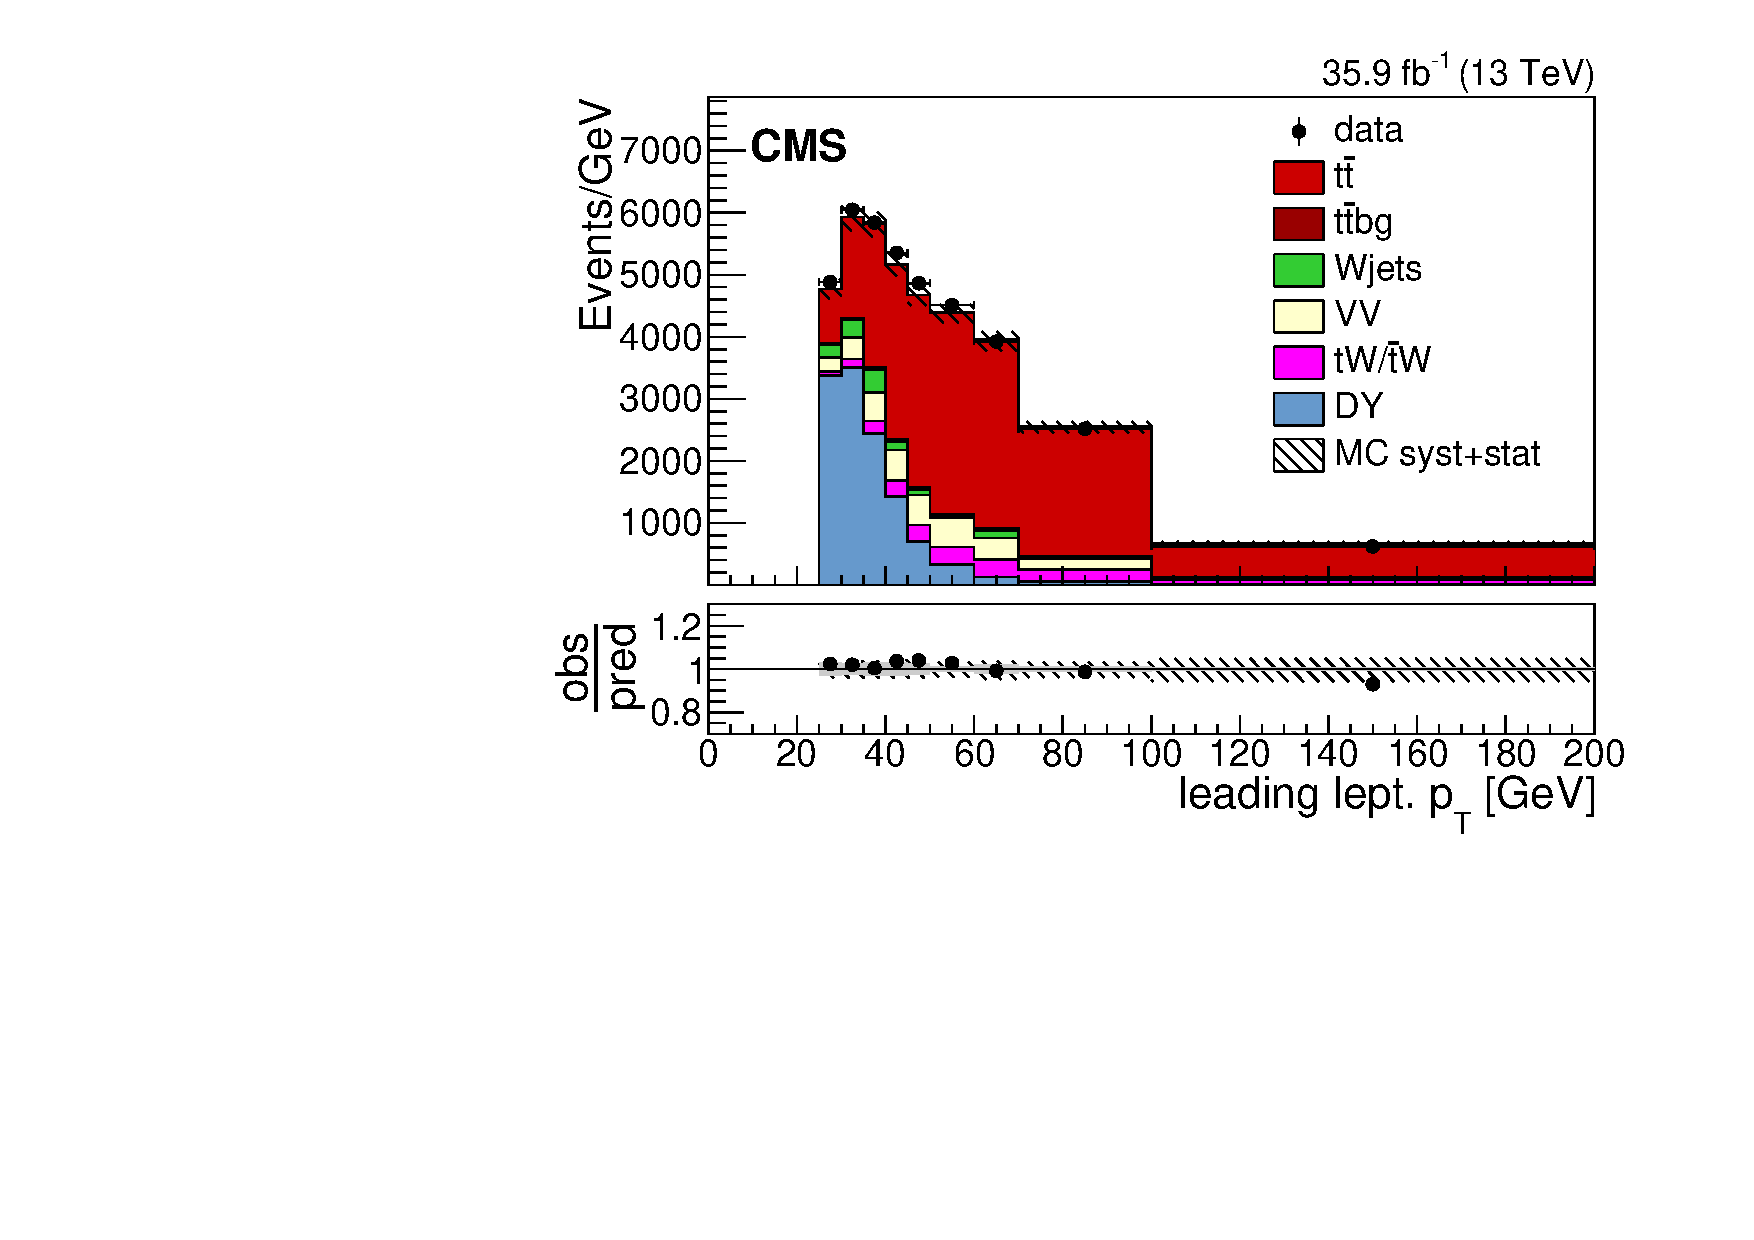
\includegraphics{CrossSection/Figures/ControlPlots/emu_sysnom/lead_lepton_pt_step_8.pdf}}
    \resizebox{0.48 \textwidth}{!}{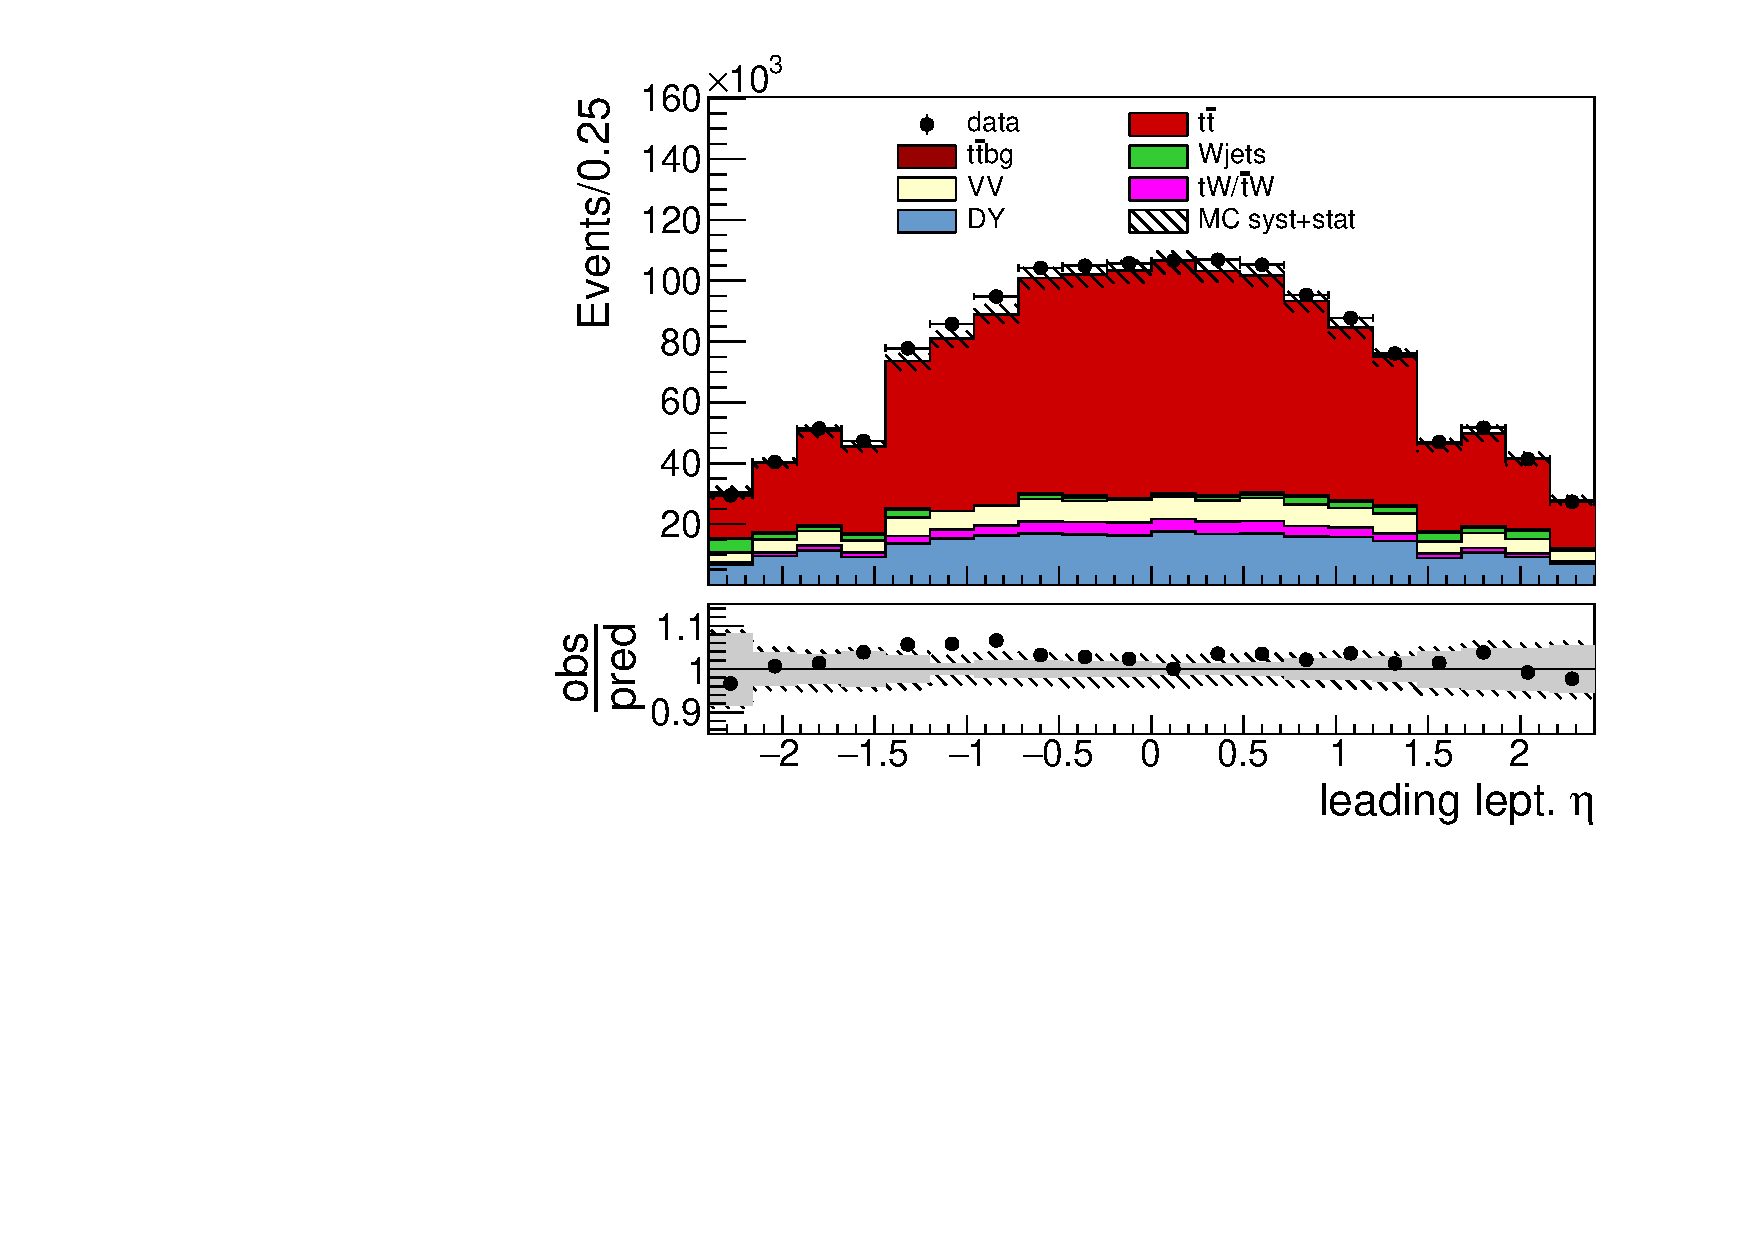
\includegraphics{CrossSection/Figures/ControlPlots/emu_sysnom/lead_lepton_eta_step_8.pdf}}
    \resizebox{0.48 \textwidth}{!}{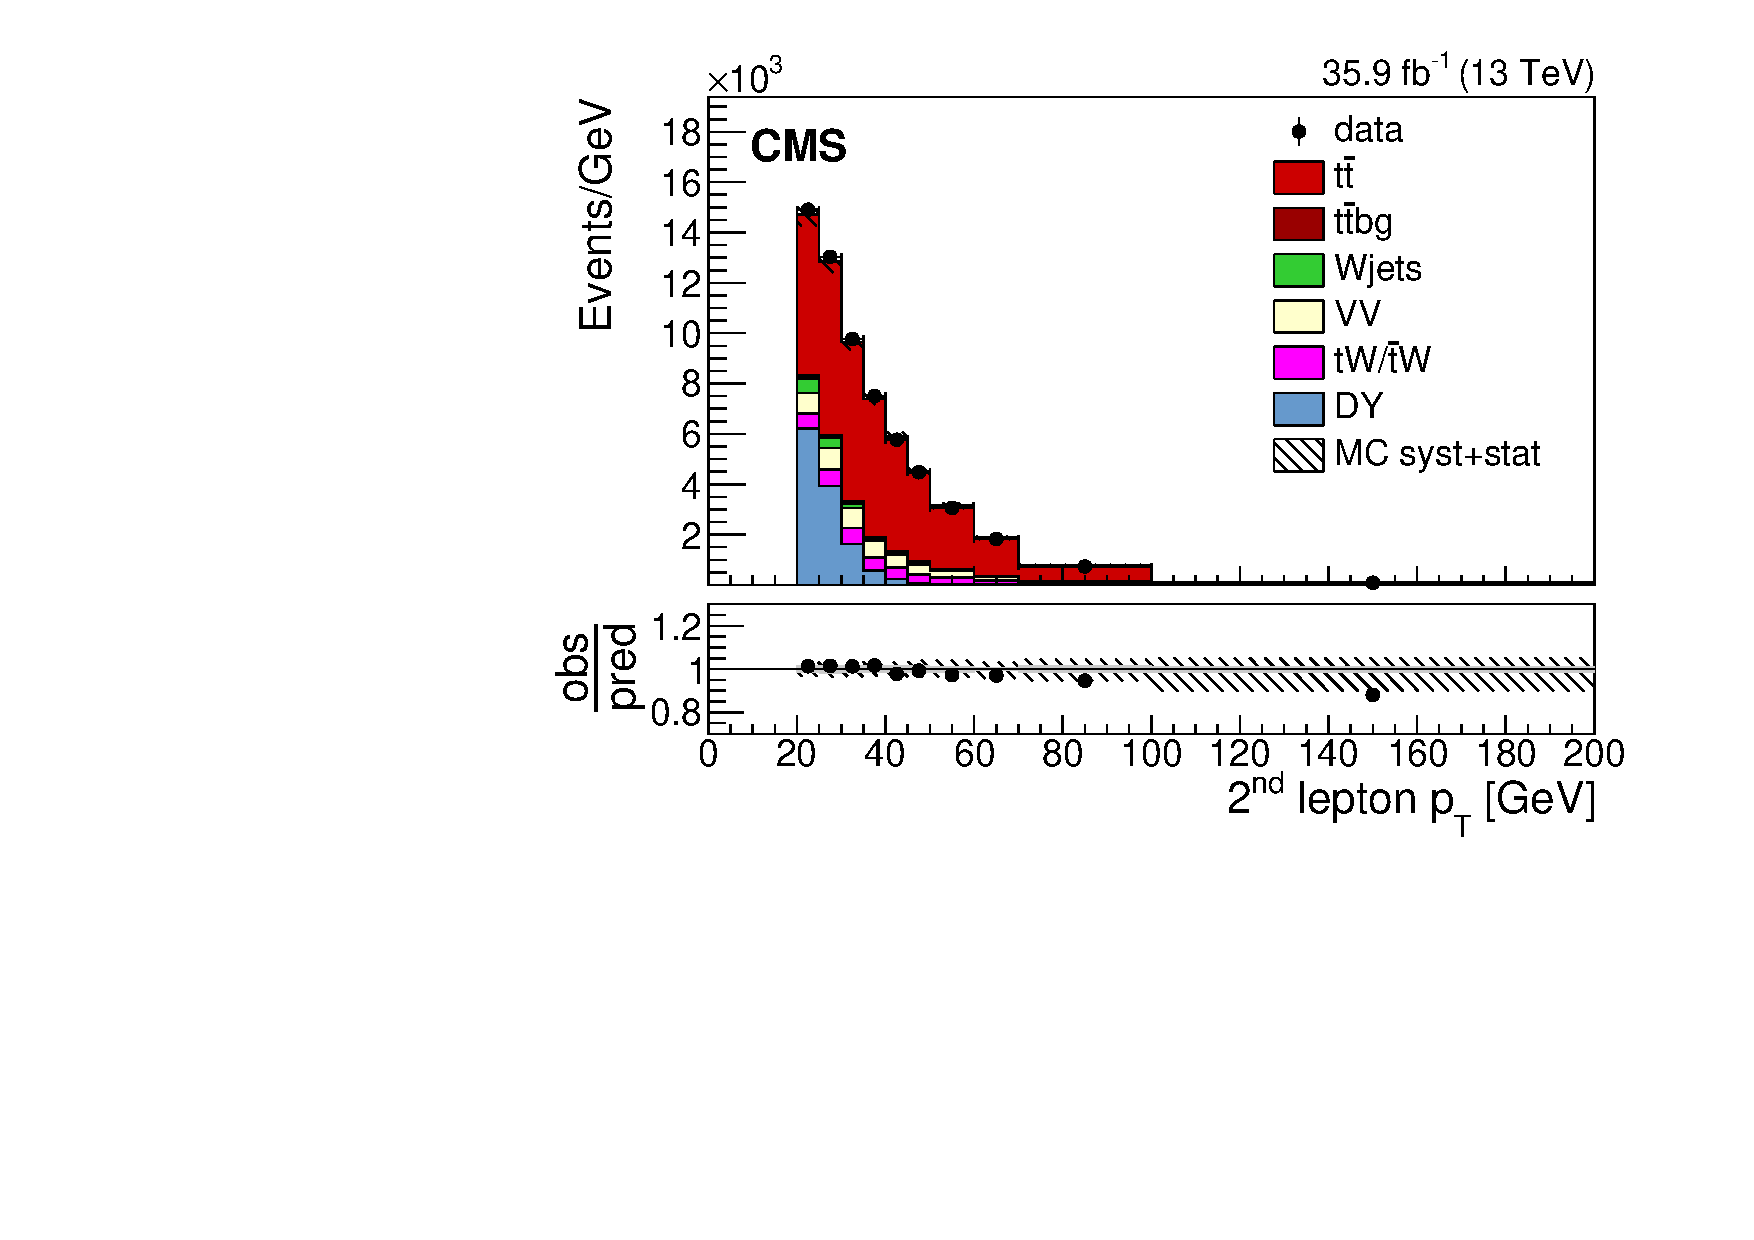
\includegraphics{CrossSection/Figures/ControlPlots/emu_sysnom/seclead_lepton_pt_step_8.pdf}}
    \resizebox{0.48 \textwidth}{!}{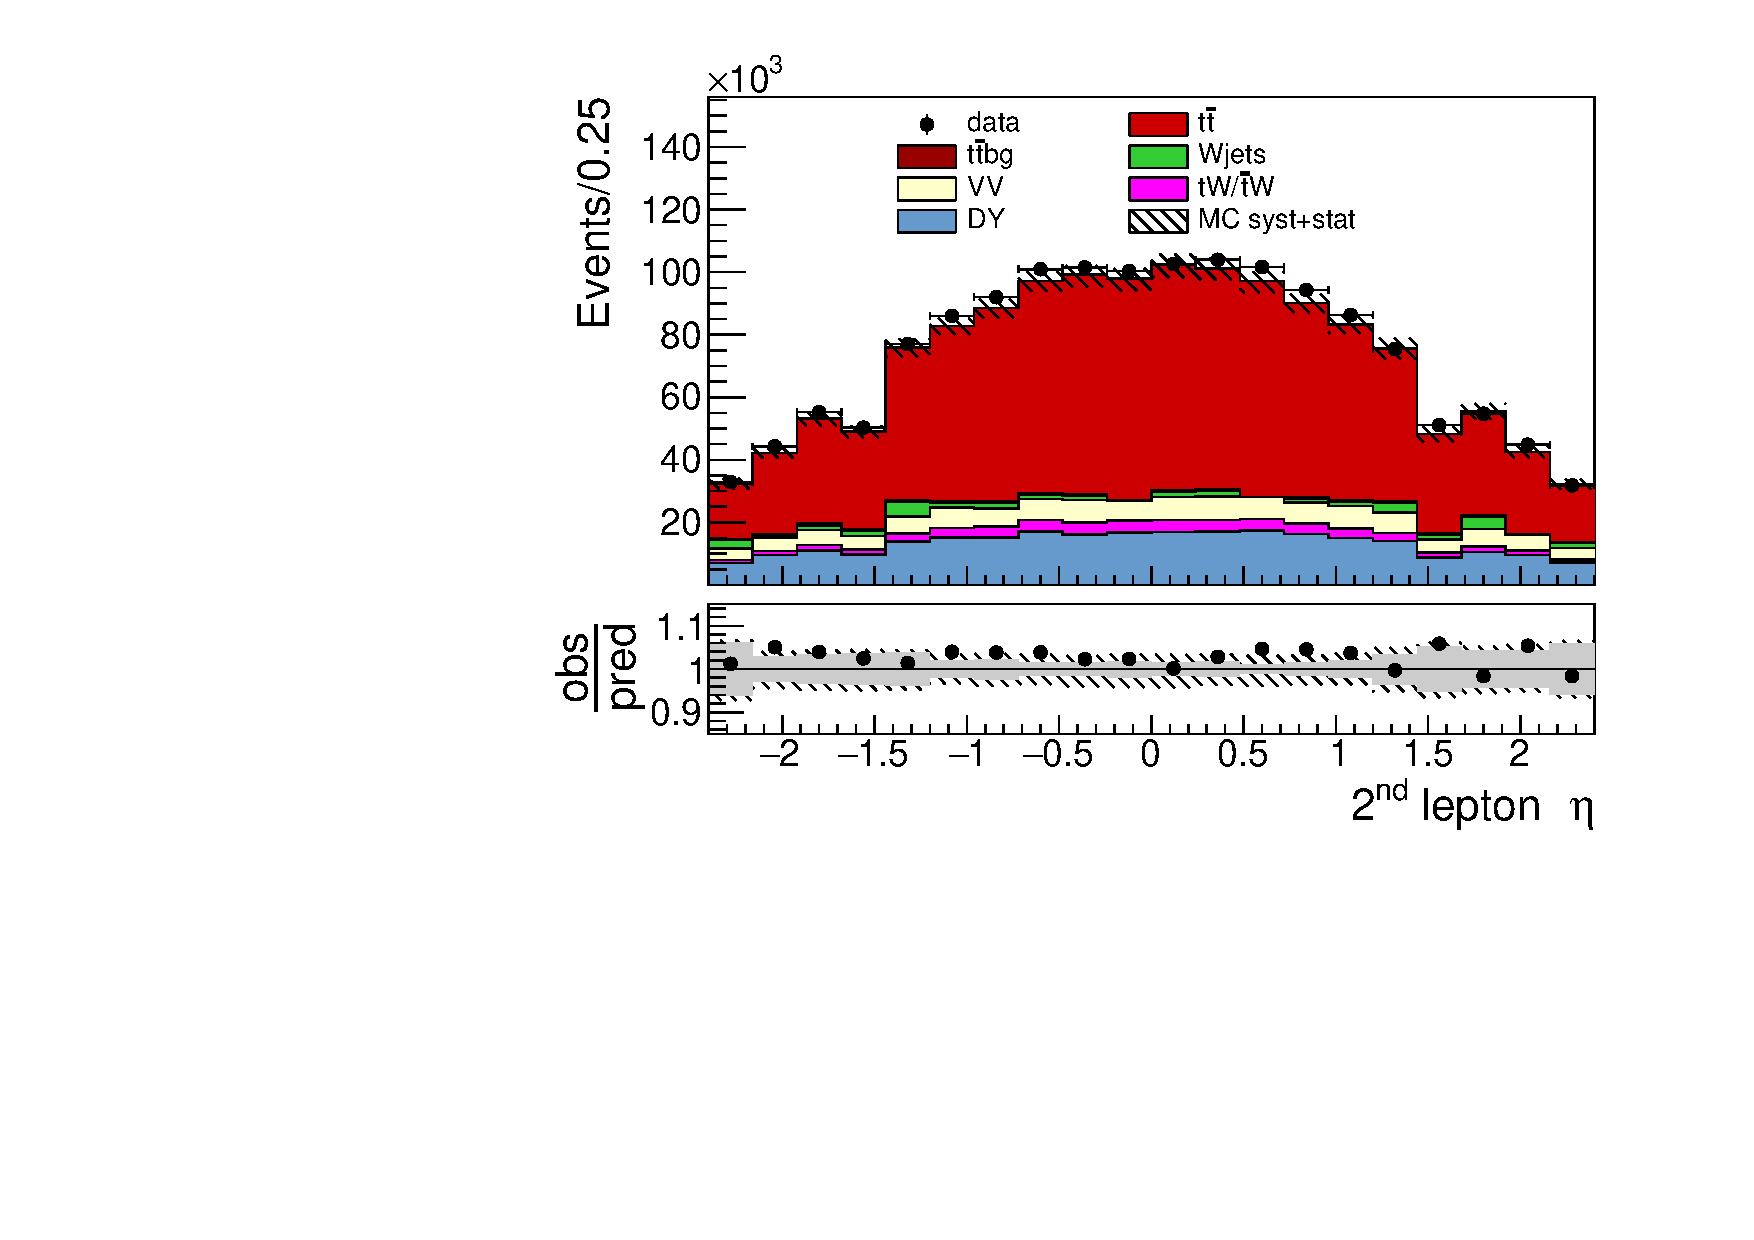
\includegraphics{CrossSection/Figures/ControlPlots/emu_sysnom/seclead_lepton_eta_step_8.pdf}}
    \resizebox{0.48 \textwidth}{!}{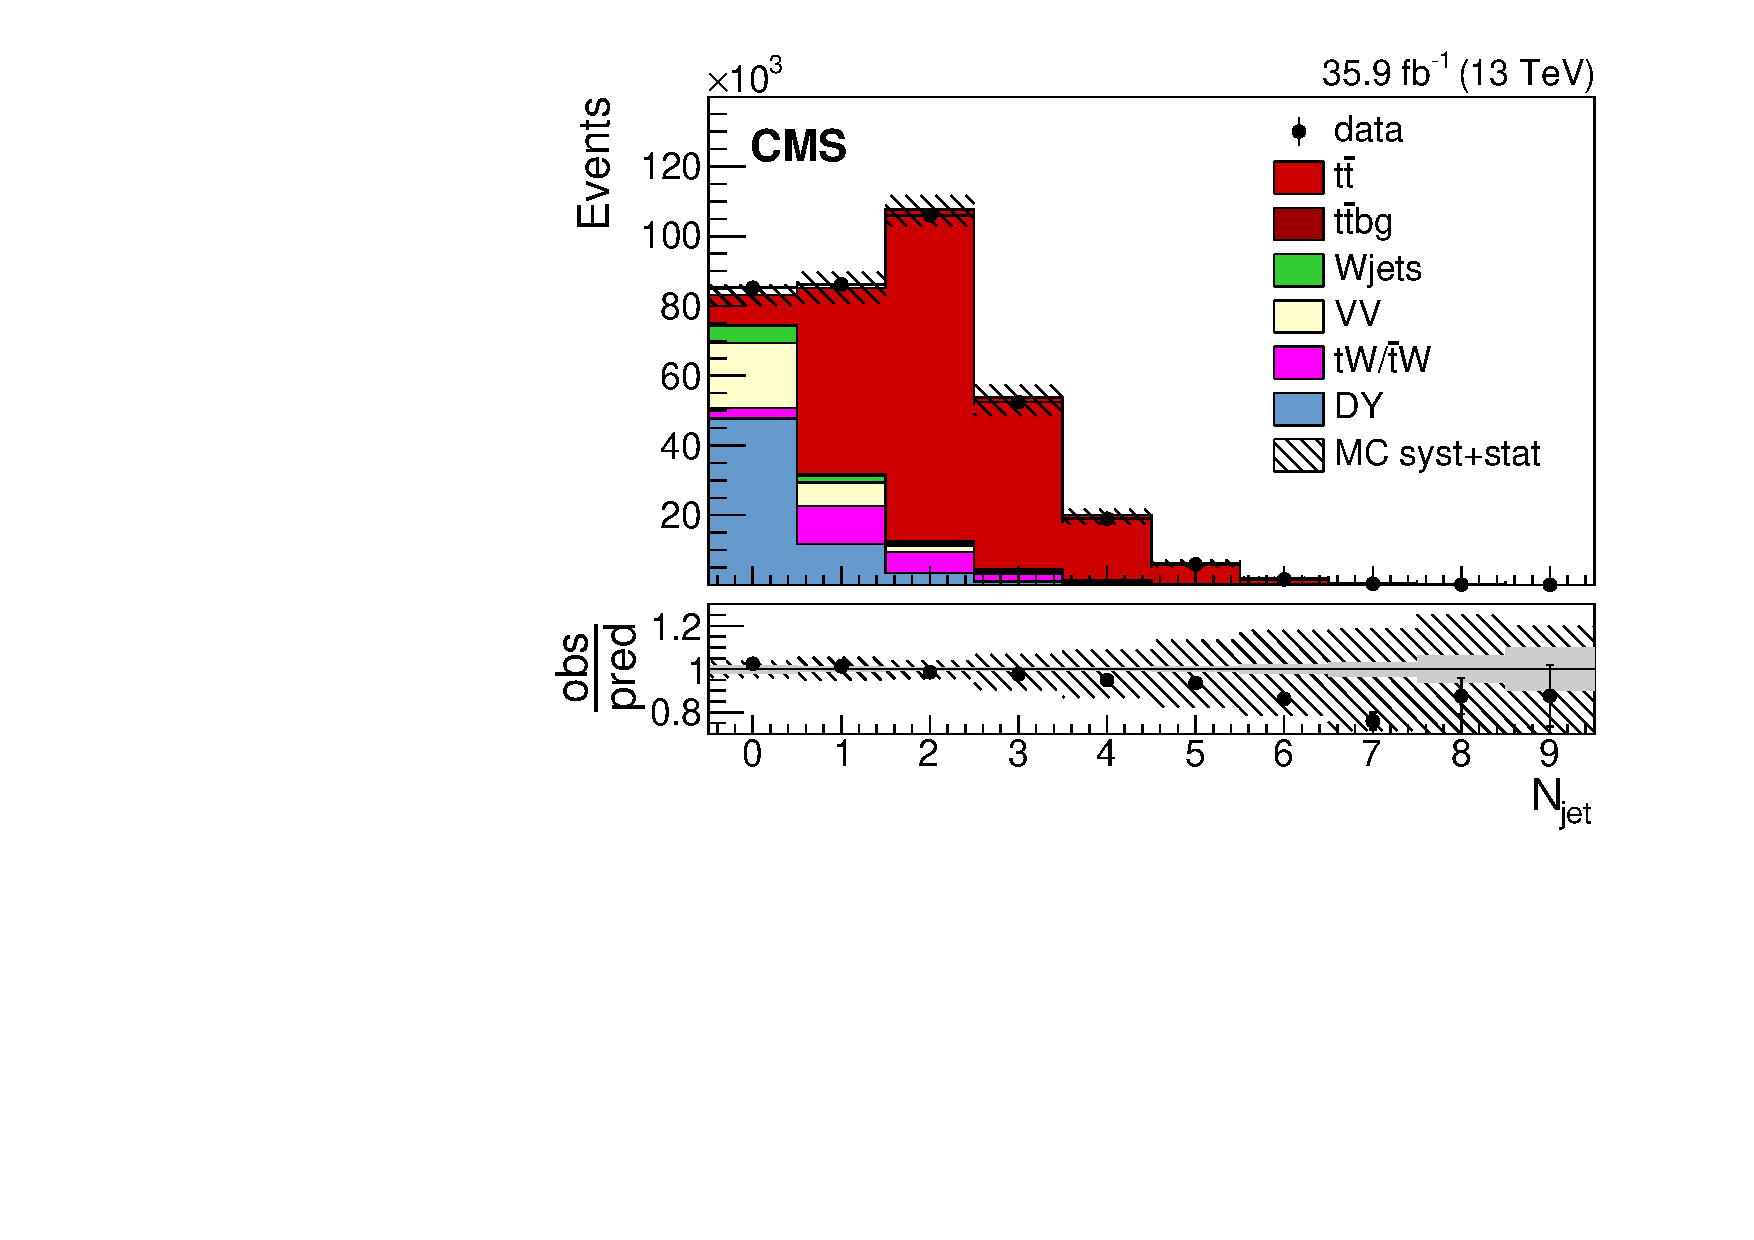
\includegraphics{CrossSection/Figures/ControlPlots/emu_sysnom/selected_jets_multi_step_8.pdf}}
    \resizebox{0.48 \textwidth}{!}{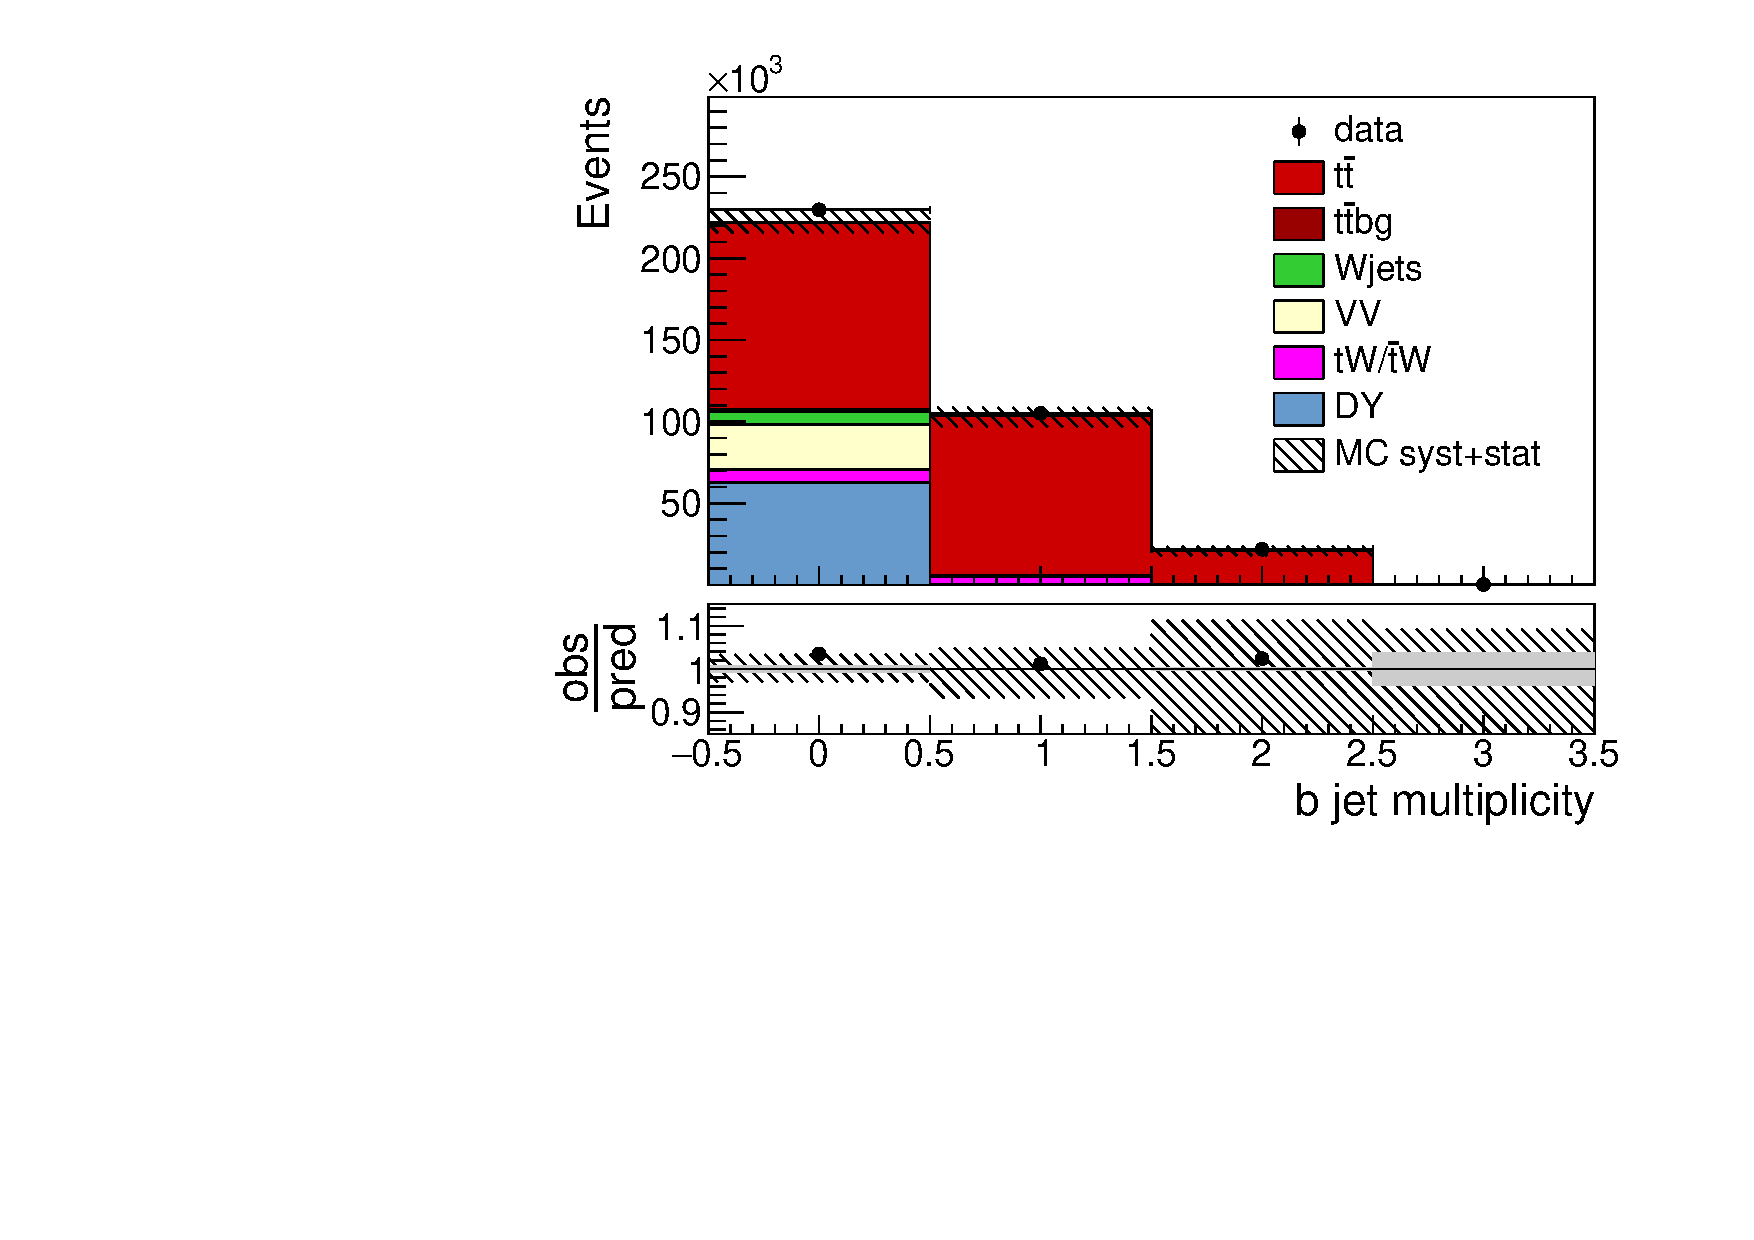
\includegraphics{CrossSection/Figures/ControlPlots/emu_sysnom/selected_b-jet_multi_step_8.pdf}}
      \caption{Transverse momentum (left) and pseudorapidity (right)
        of leading (first row) and second-leading (second row) lepton in the \emu channel after the
        event selection required by the \ttbar cross section
        extraction technique based on a simultaneous fit.
        Jet and b-jet multiplicity after the same selection steps are
        shown in the third row. The hatched
        bands correspond to the total uncertainty on the sum of the
        predicted yields. 
        %agrohsje , excluding luminosity and background
        %normalization uncertainties. 
        The ratios of data to the sum of the predicted yields are
        shown at the bottom of each plot. Here, the solid gray band
        represents the contribution of the statistical uncertainty.}  
       \label{fig:xsec_emu_ctrplots}
  \end{center}
\end{figure}

\begin{figure}[htbp!]
  \begin{center}
    \resizebox{0.48 \textwidth}{!}{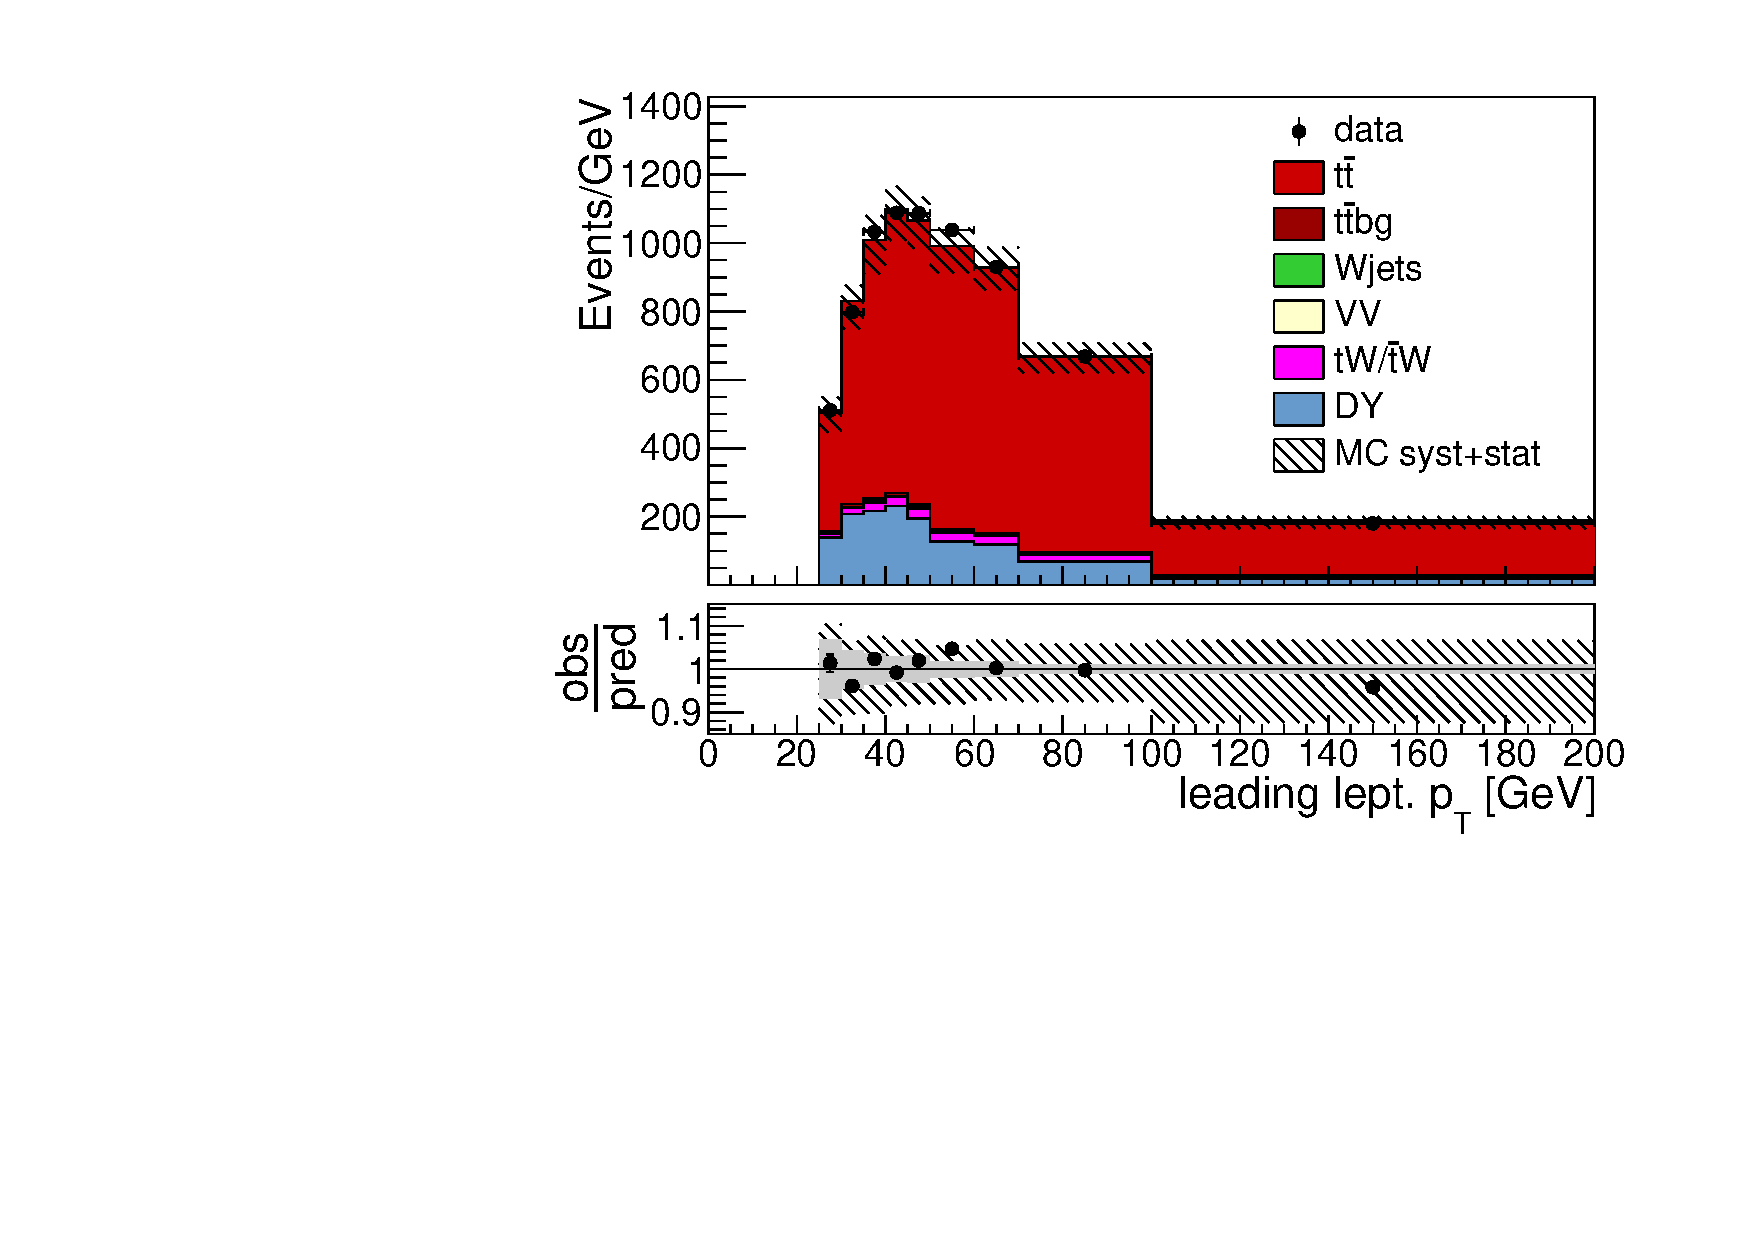
\includegraphics{CrossSection/Figures/ControlPlots/mumu_sysnom/lead_lepton_pt_step_8.pdf}}
    \resizebox{0.48 \textwidth}{!}{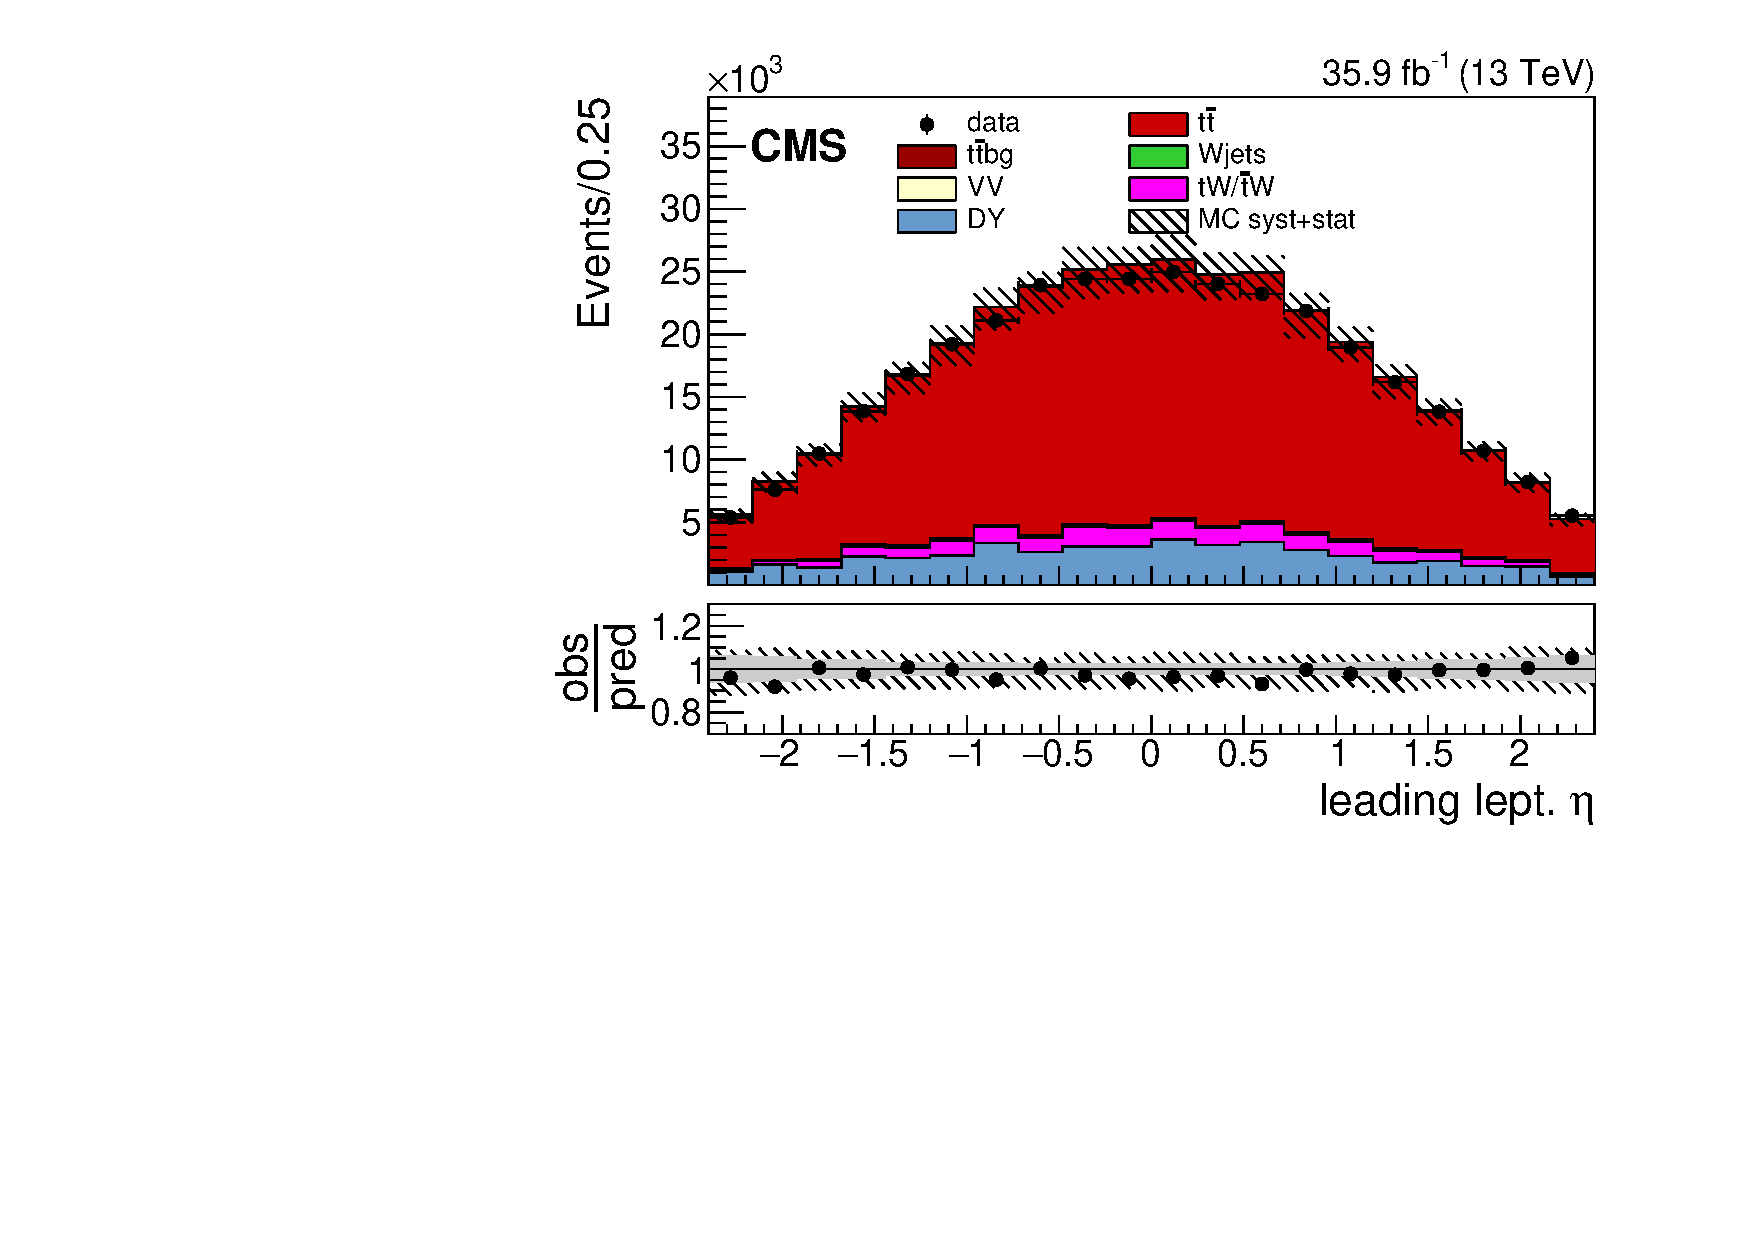
\includegraphics{CrossSection/Figures/ControlPlots/mumu_sysnom/lead_lepton_eta_step_8.pdf}}
    \resizebox{0.48 \textwidth}{!}{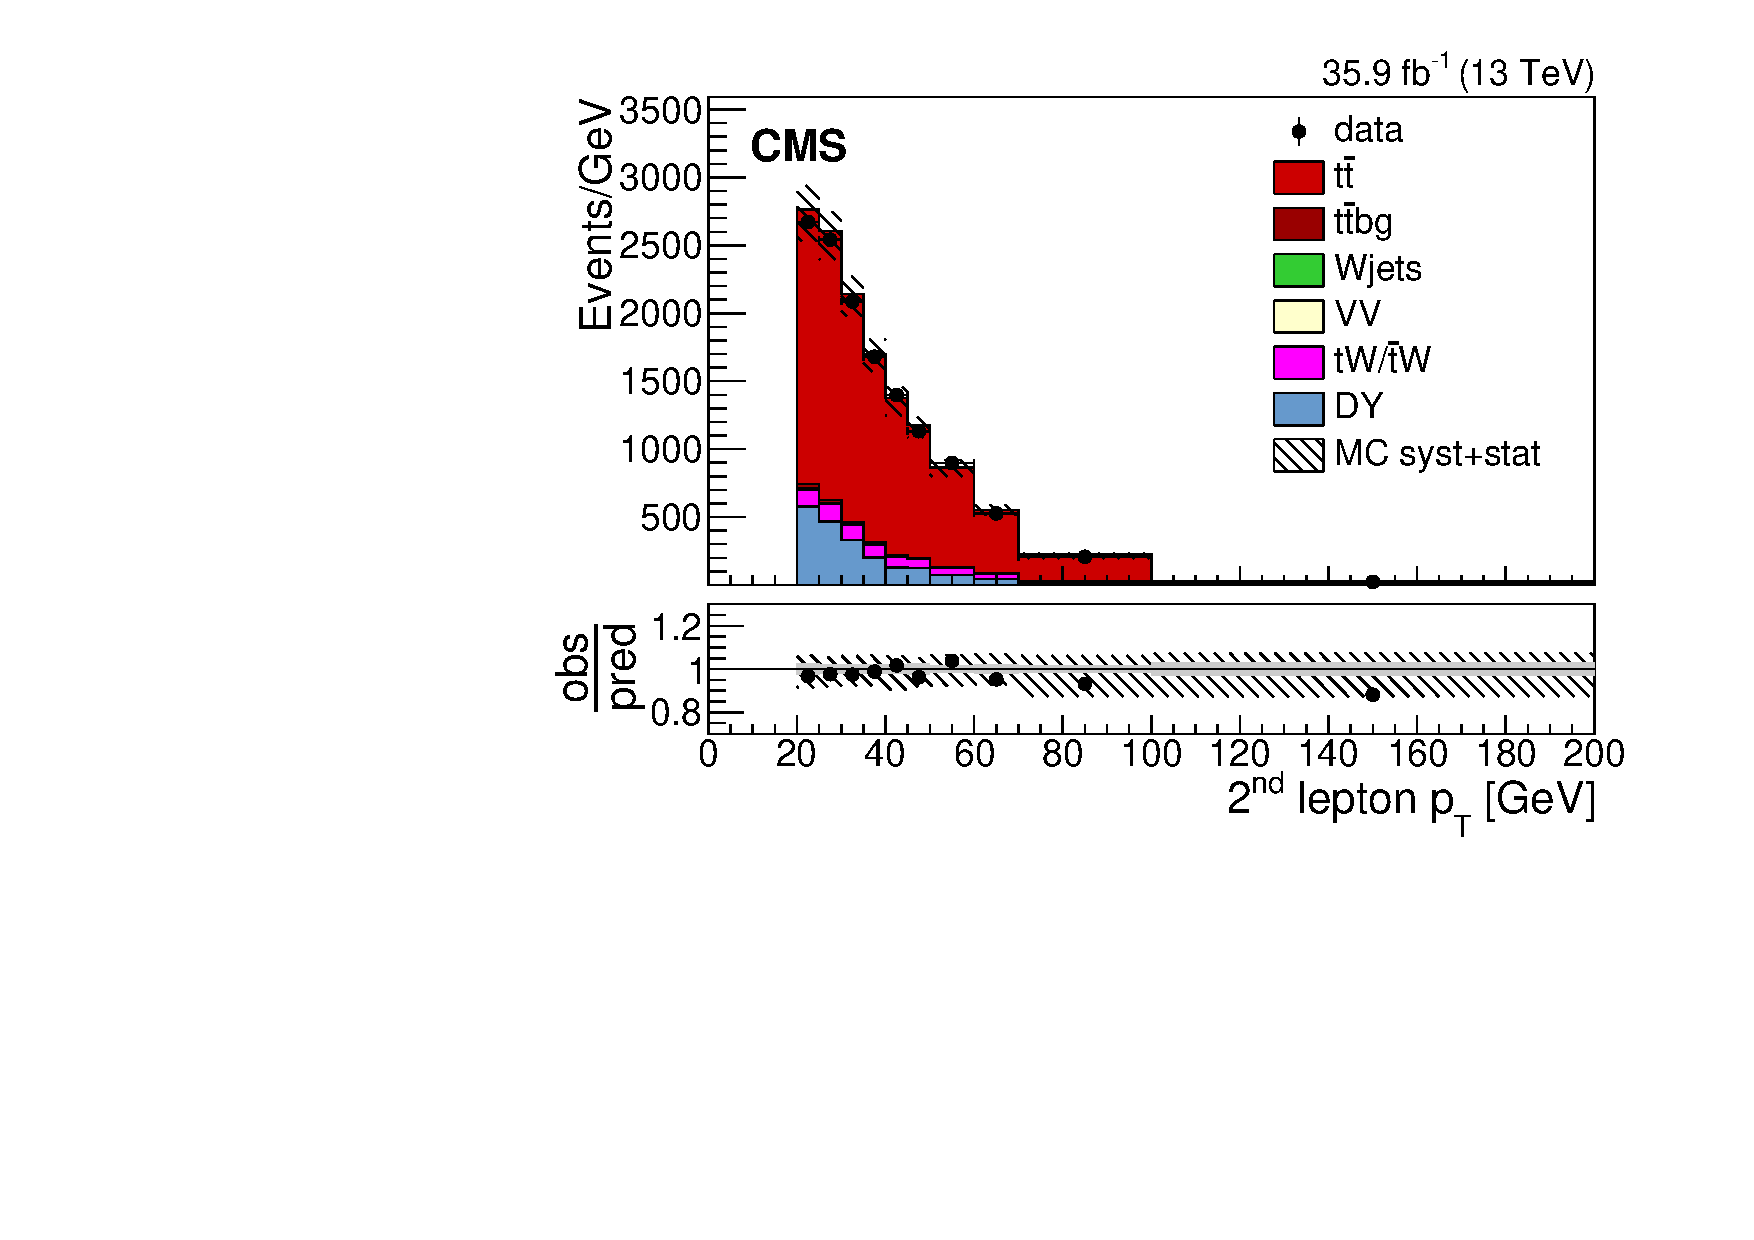
\includegraphics{CrossSection/Figures/ControlPlots/mumu_sysnom/seclead_lepton_pt_step_8.pdf}}
    \resizebox{0.48 \textwidth}{!}{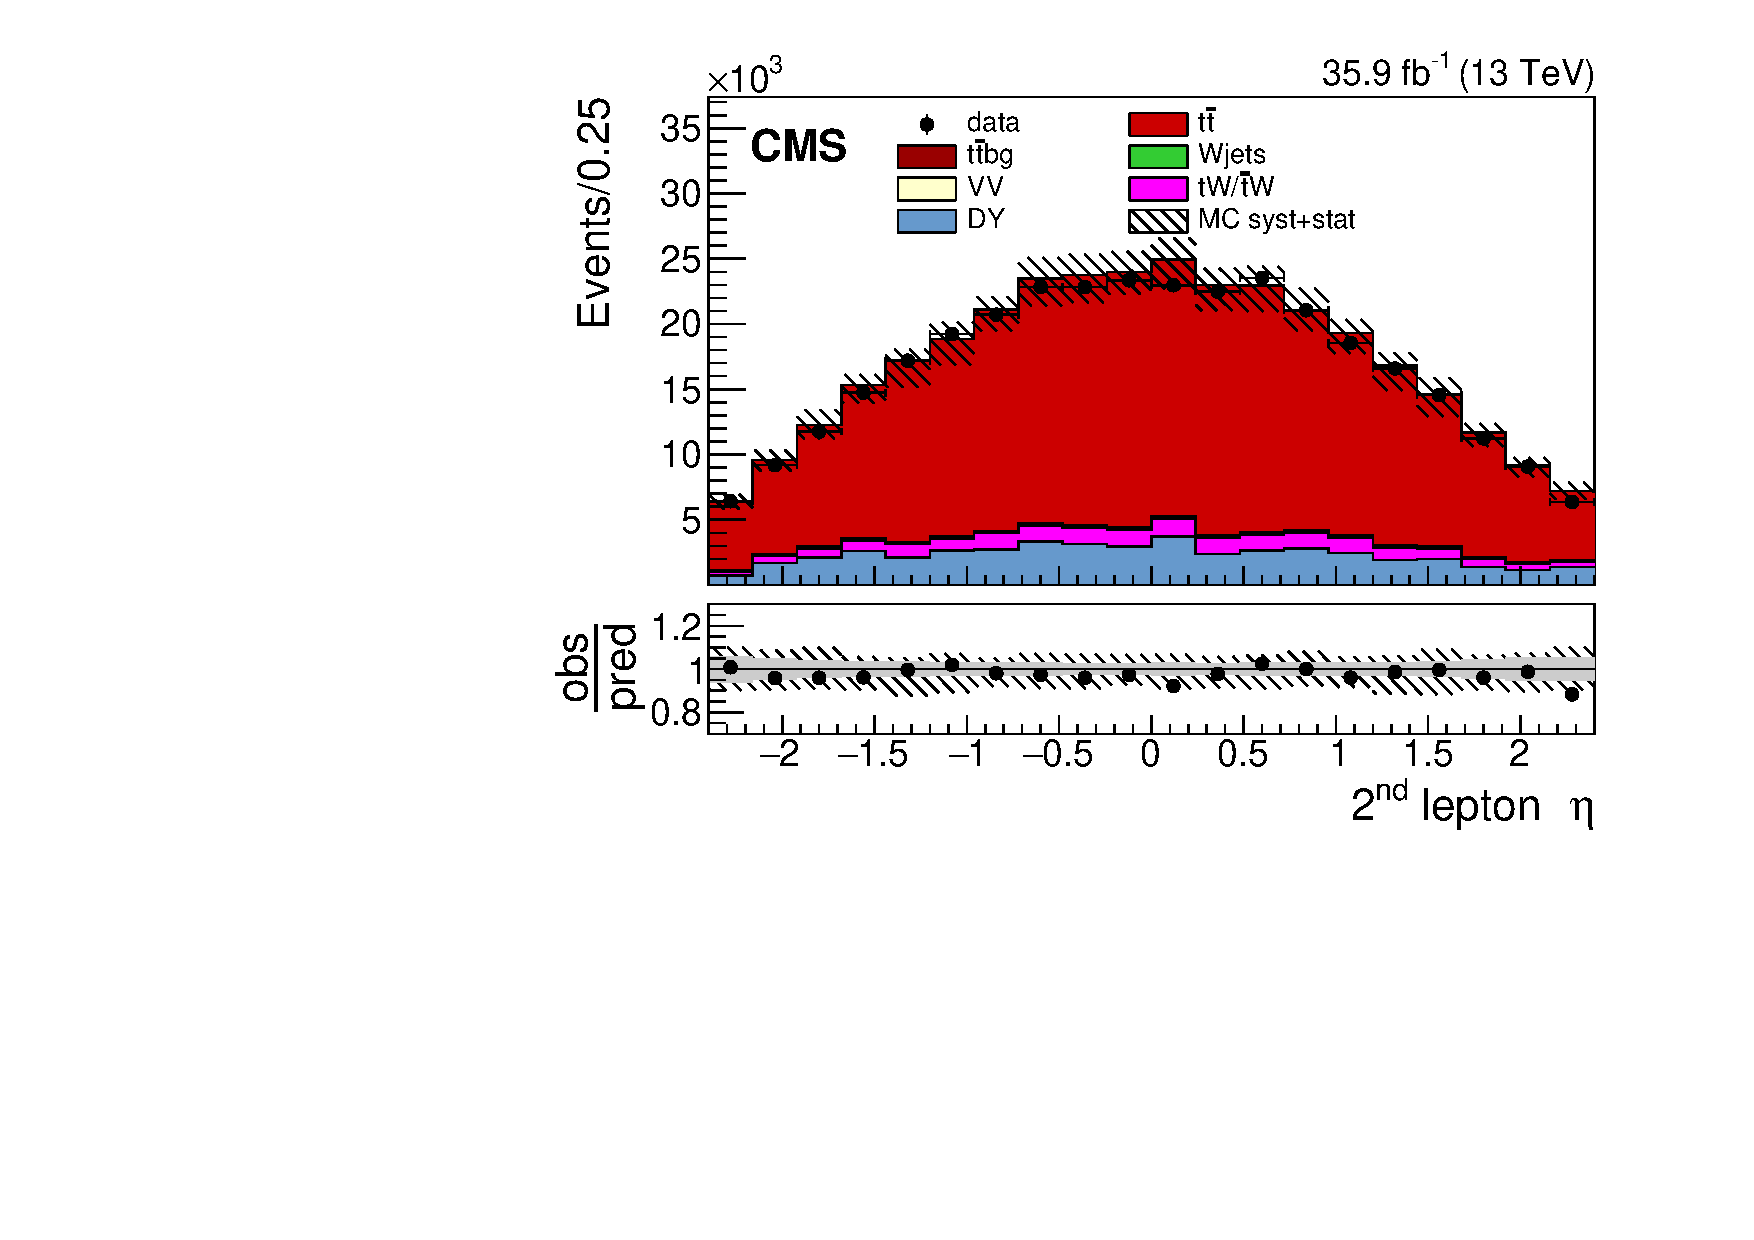
\includegraphics{CrossSection/Figures/ControlPlots/mumu_sysnom/seclead_lepton_eta_step_8.pdf}}
    \resizebox{0.48 \textwidth}{!}{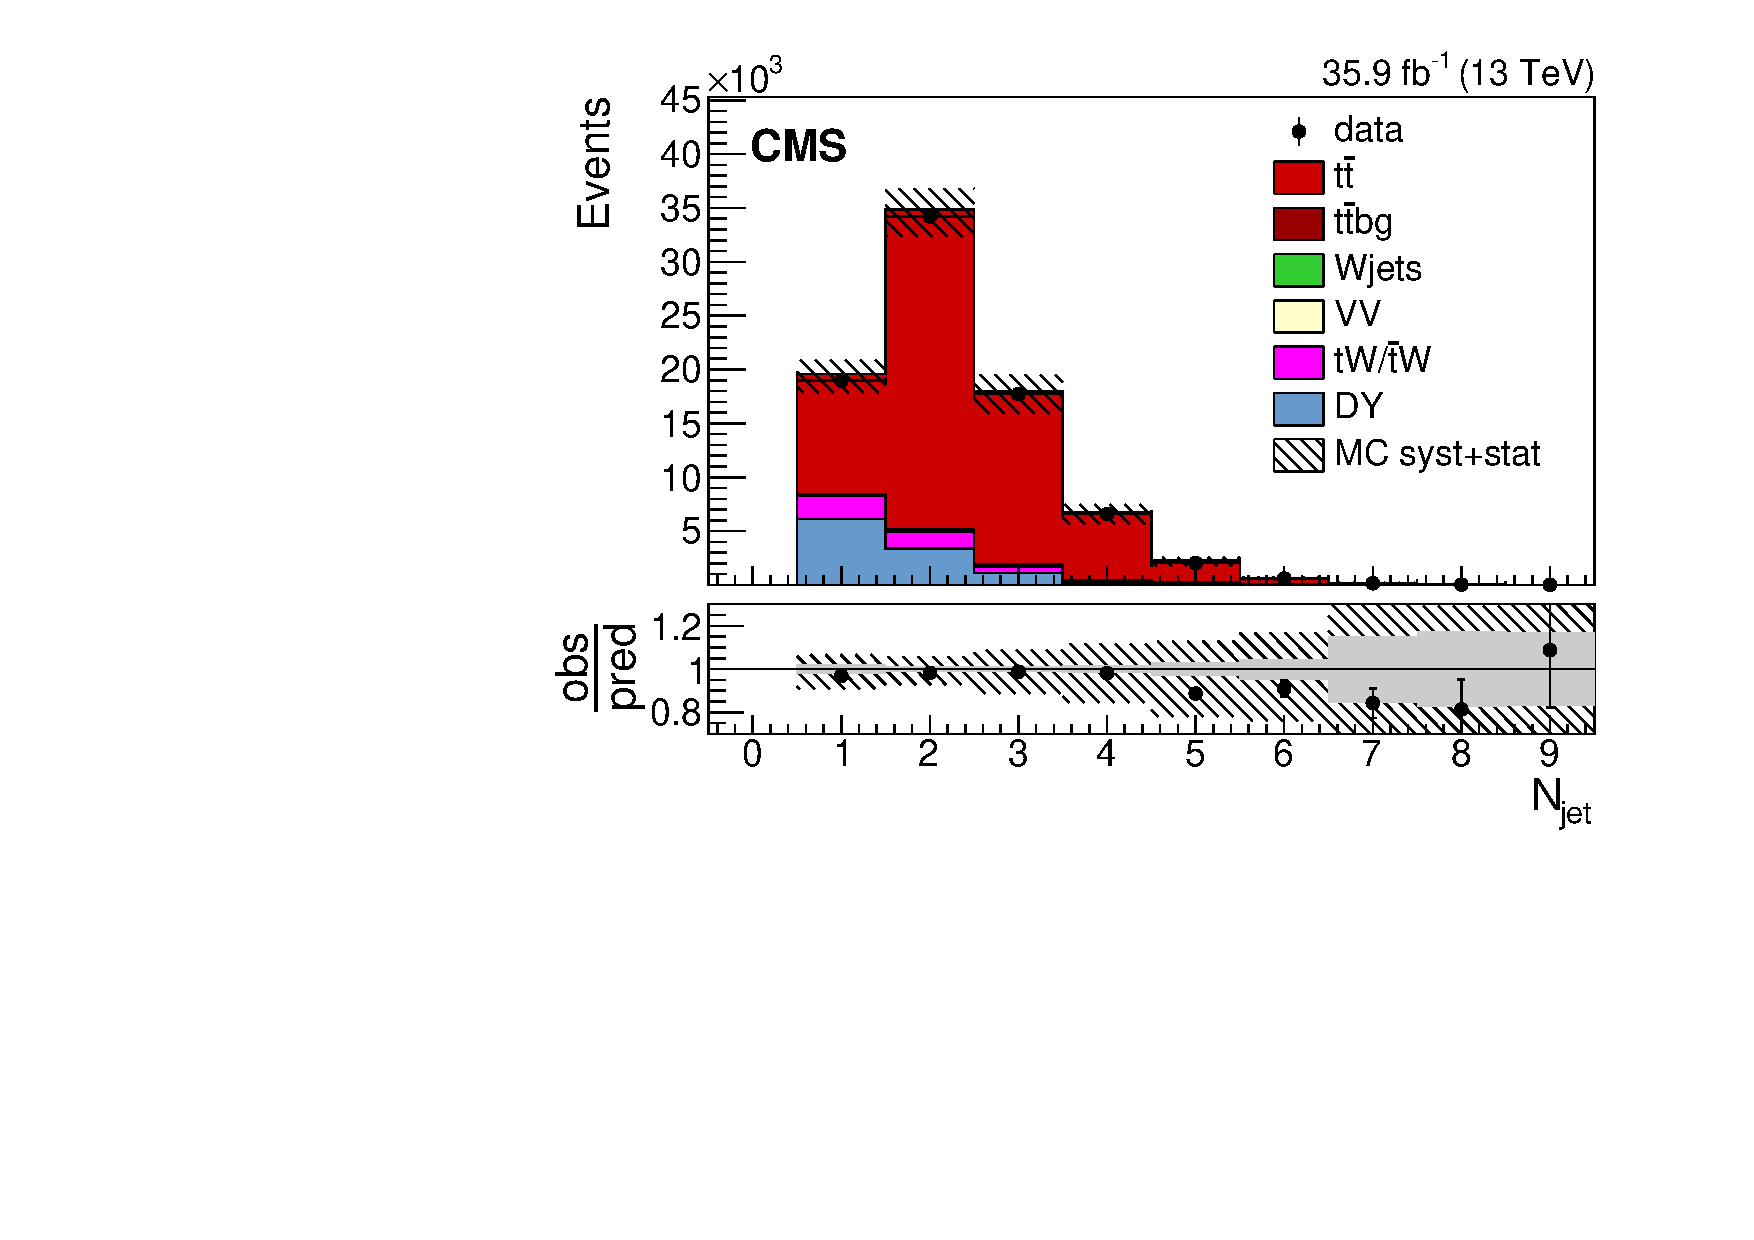
\includegraphics{CrossSection/Figures/ControlPlots/mumu_sysnom/selected_jets_multi_step_8.pdf}}
    \resizebox{0.48 \textwidth}{!}{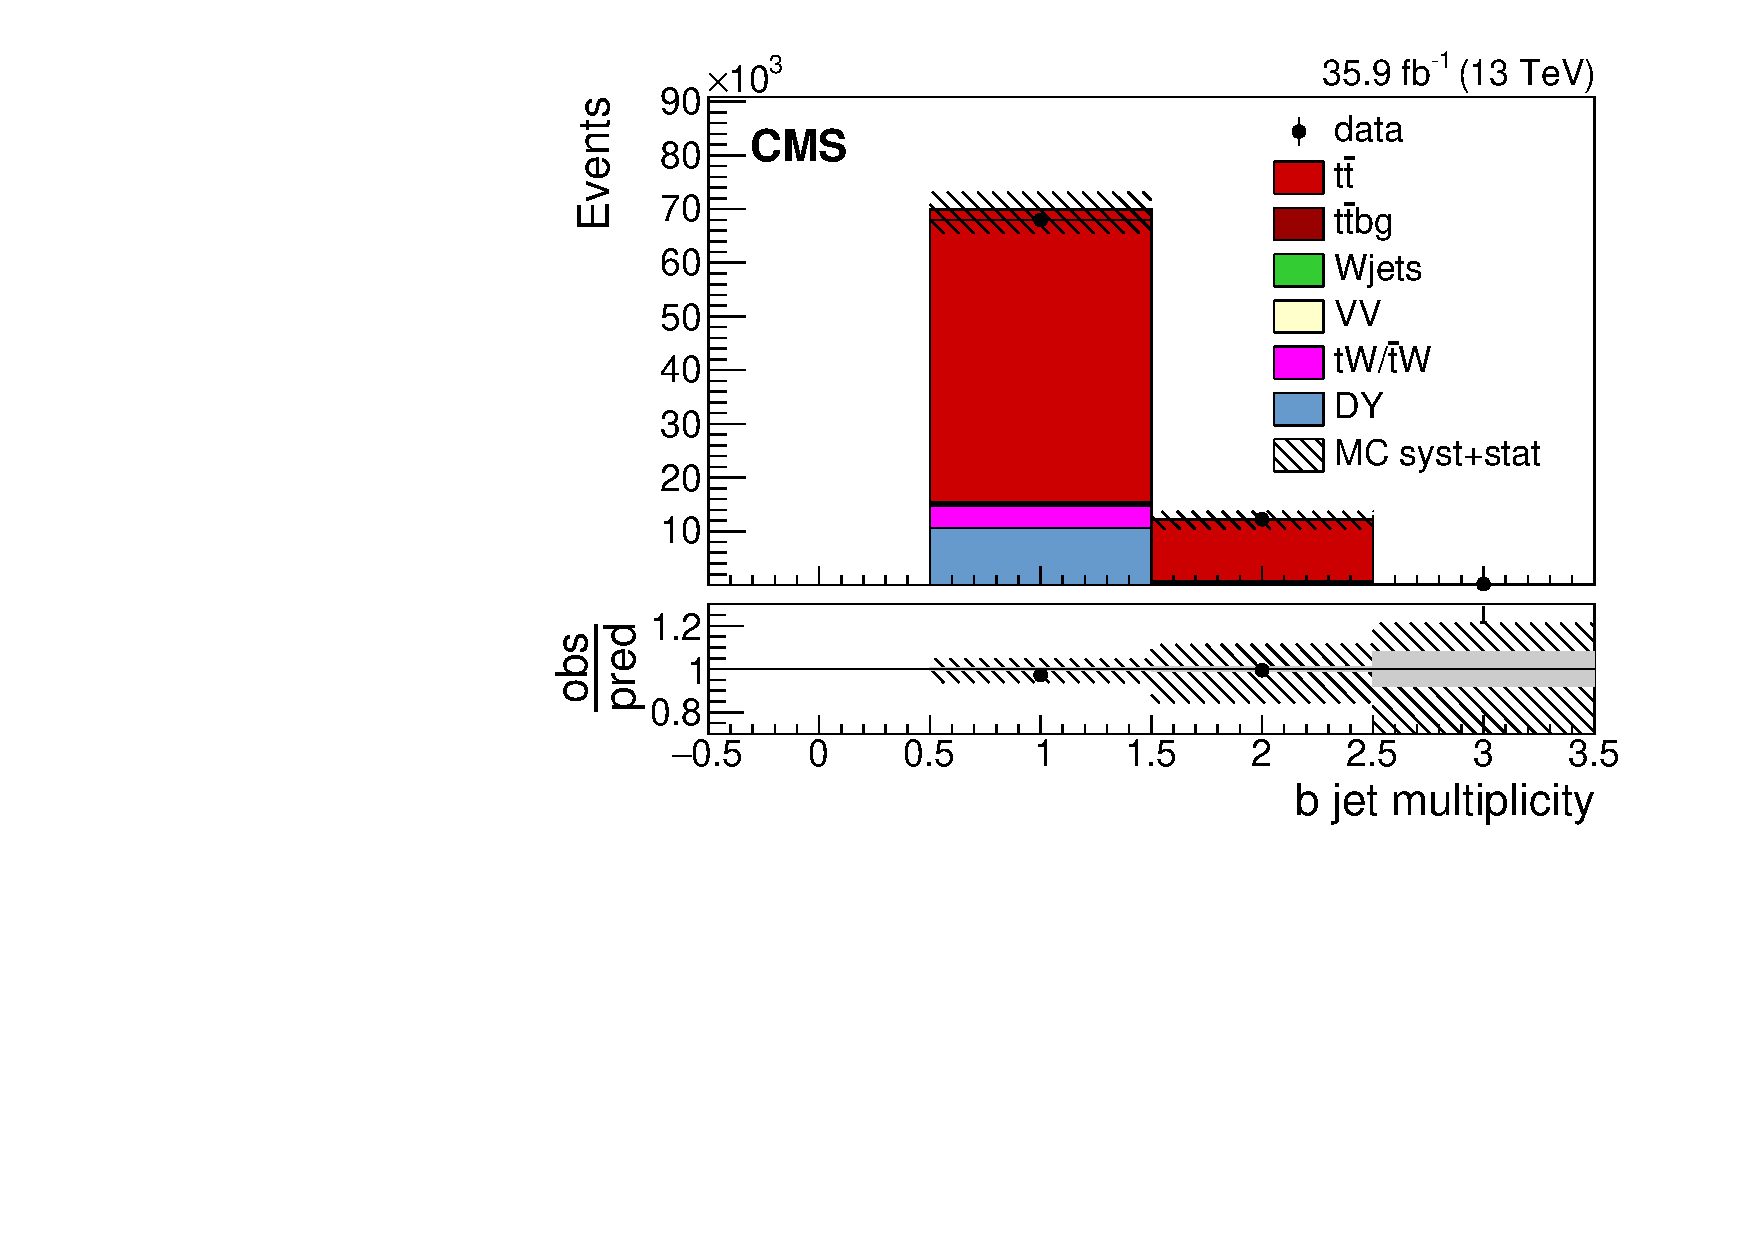
\includegraphics{CrossSection/Figures/ControlPlots/mumu_sysnom/selected_b-jet_multi_step_8.pdf}}
      \caption{Transverse momentum (left) and pseudorapidity (right)
        of leading (first row) and second-leading (second row) lepton in the \mumu channel after the
        event selection required by the \ttbar cross section
        extraction technique based on a simultaneous fit. Jet and b-jet multiplicity after the same selection steps are
        shown in the third row. The hatched
        bands correspond to the total uncertainty on the sum of the
        predicted yields. 
        %agrohsje , excluding luminosity and background
        %normalization uncertainties. 
        The ratios of data to the sum of the predicted yields are
        shown at the bottom of each plot. Here, the solid gray band
        represents the contribution of the statistical uncertainty.}  
       \label{fig:xsec_mumu_ctrplots}
  \end{center}
\end{figure}

\begin{figure}[htbp!]
  \begin{center}
    \resizebox{0.48 \textwidth}{!}{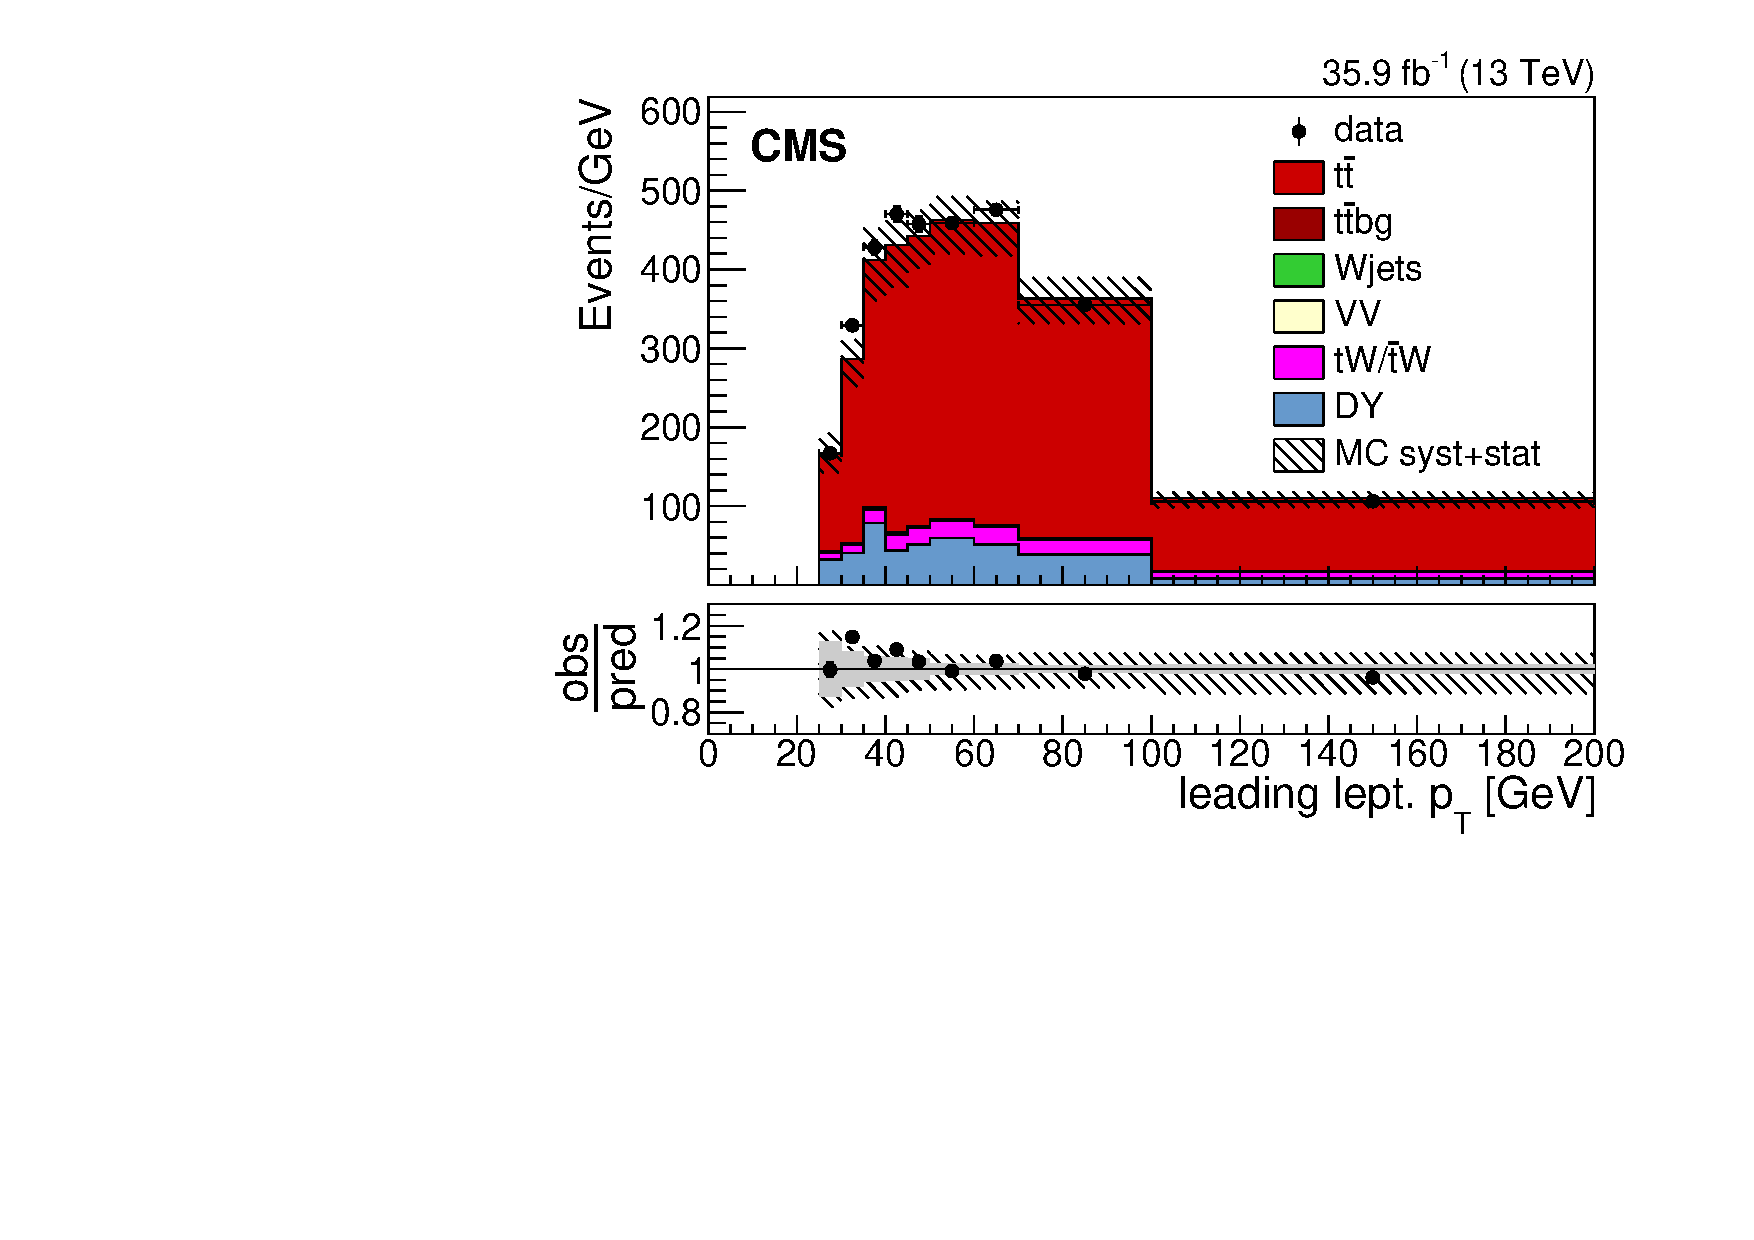
\includegraphics{CrossSection/Figures/ControlPlots/ee_sysnom/lead_lepton_pt_step_8.pdf}}
    \resizebox{0.48 \textwidth}{!}{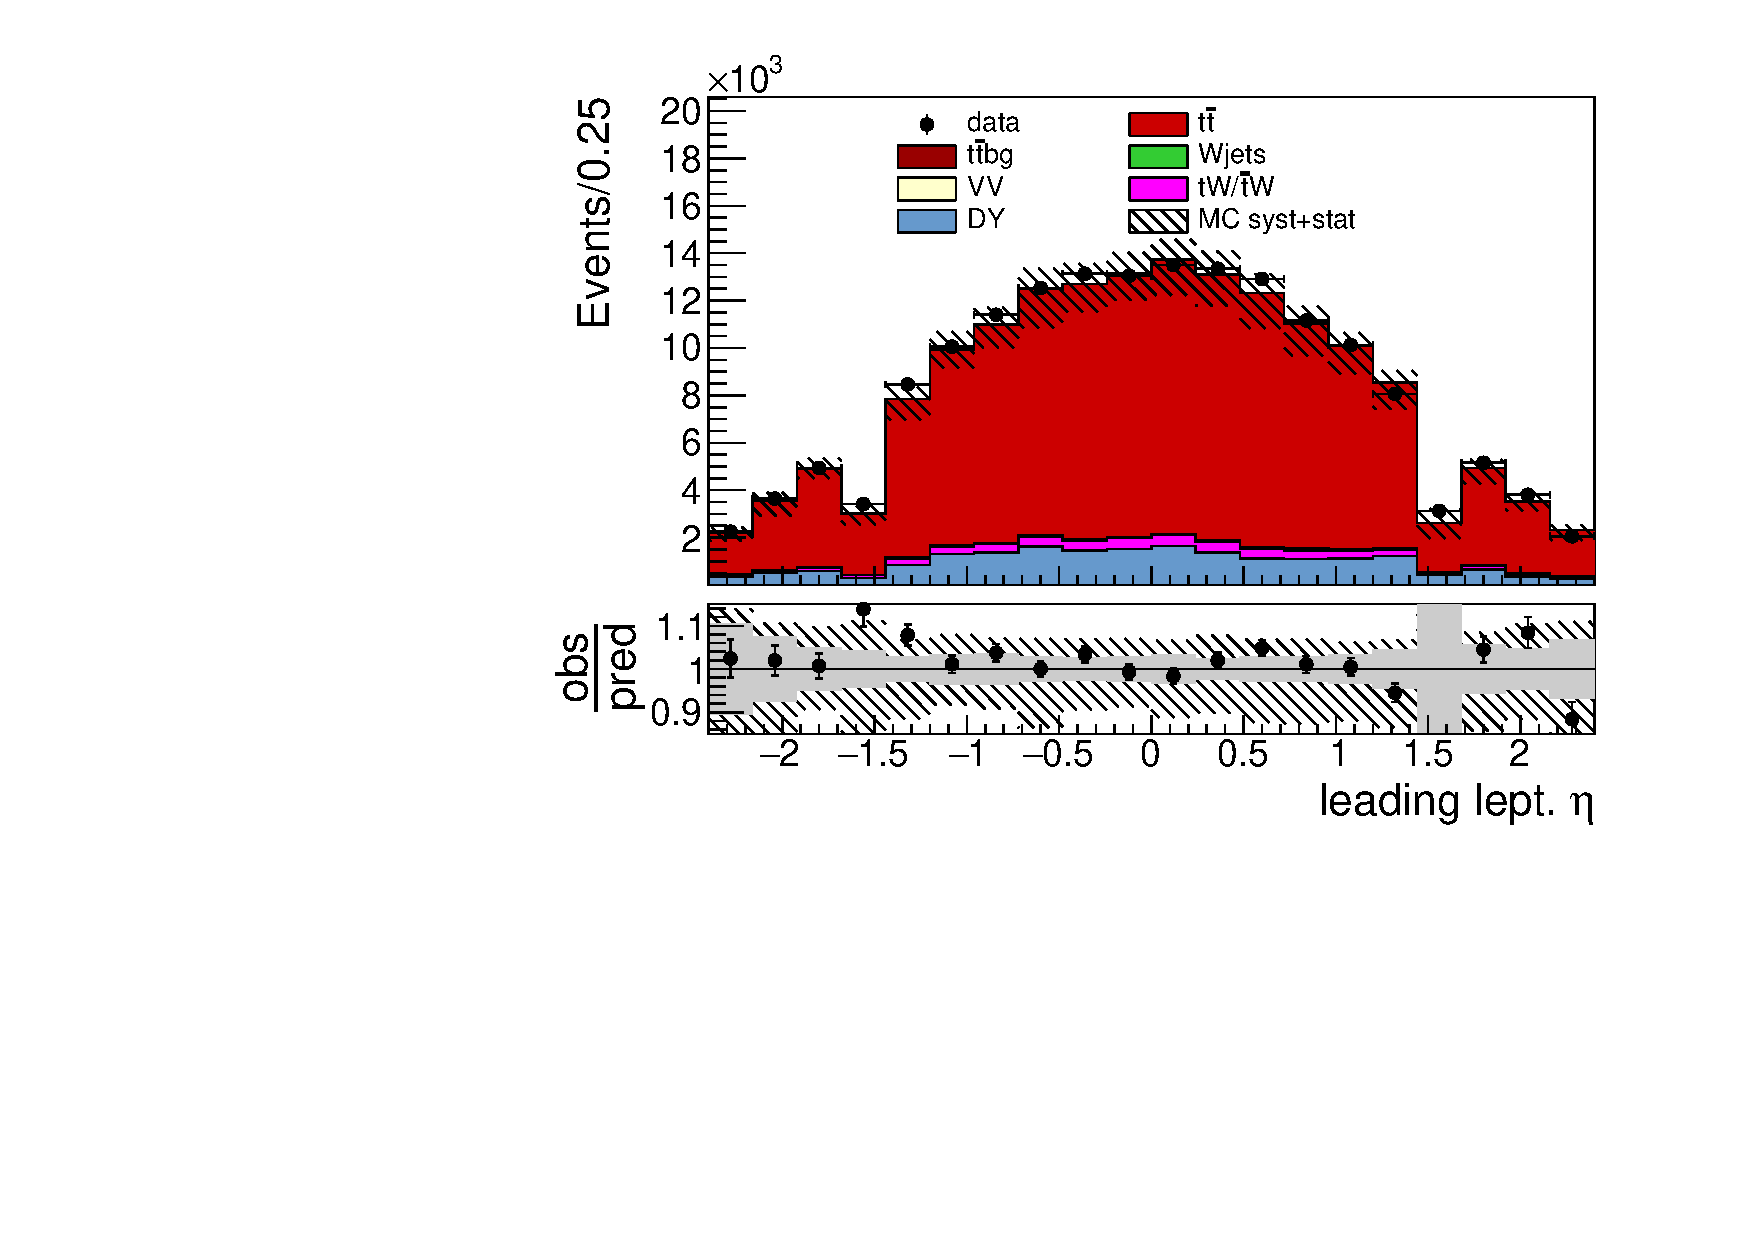
\includegraphics{CrossSection/Figures/ControlPlots/ee_sysnom/lead_lepton_eta_step_8.pdf}}
    \resizebox{0.48 \textwidth}{!}{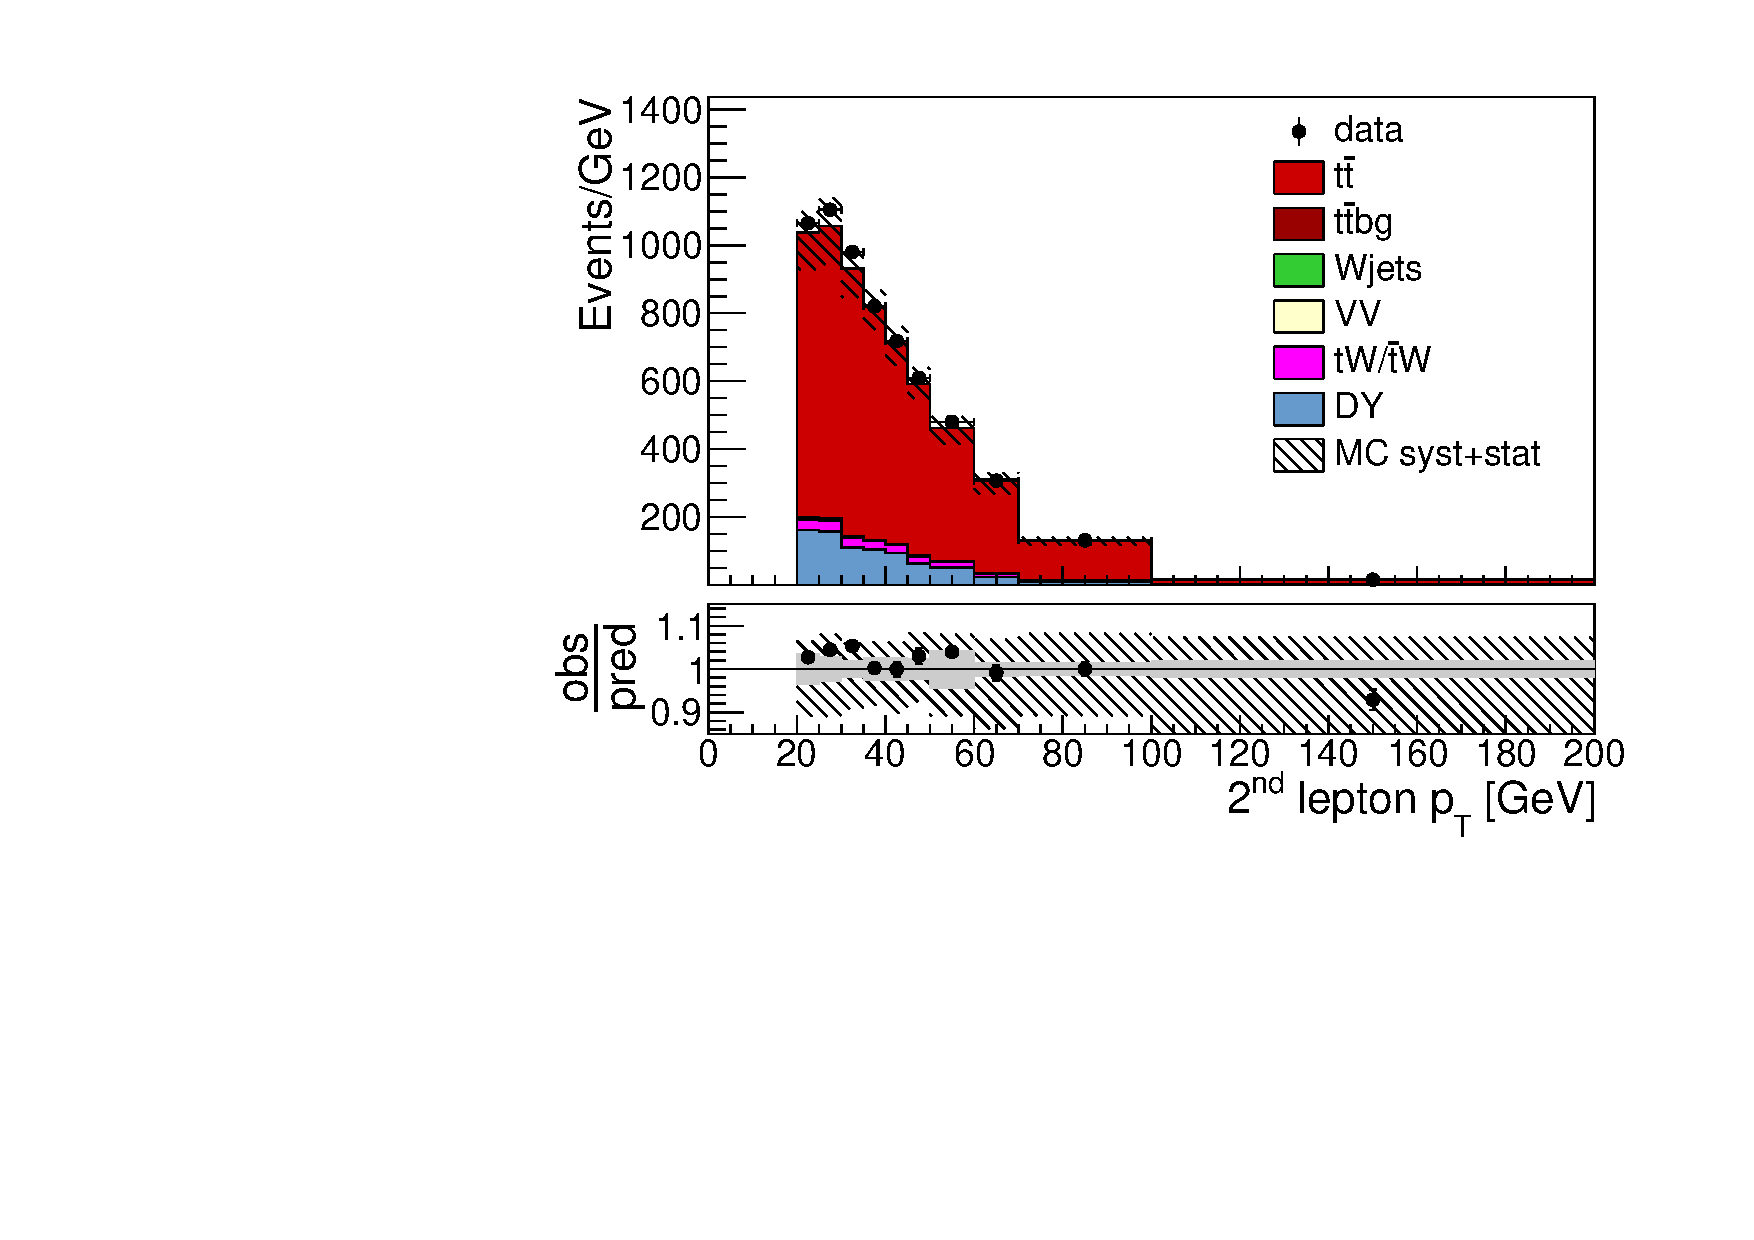
\includegraphics{CrossSection/Figures/ControlPlots/ee_sysnom/seclead_lepton_pt_step_8.pdf}}
    \resizebox{0.48 \textwidth}{!}{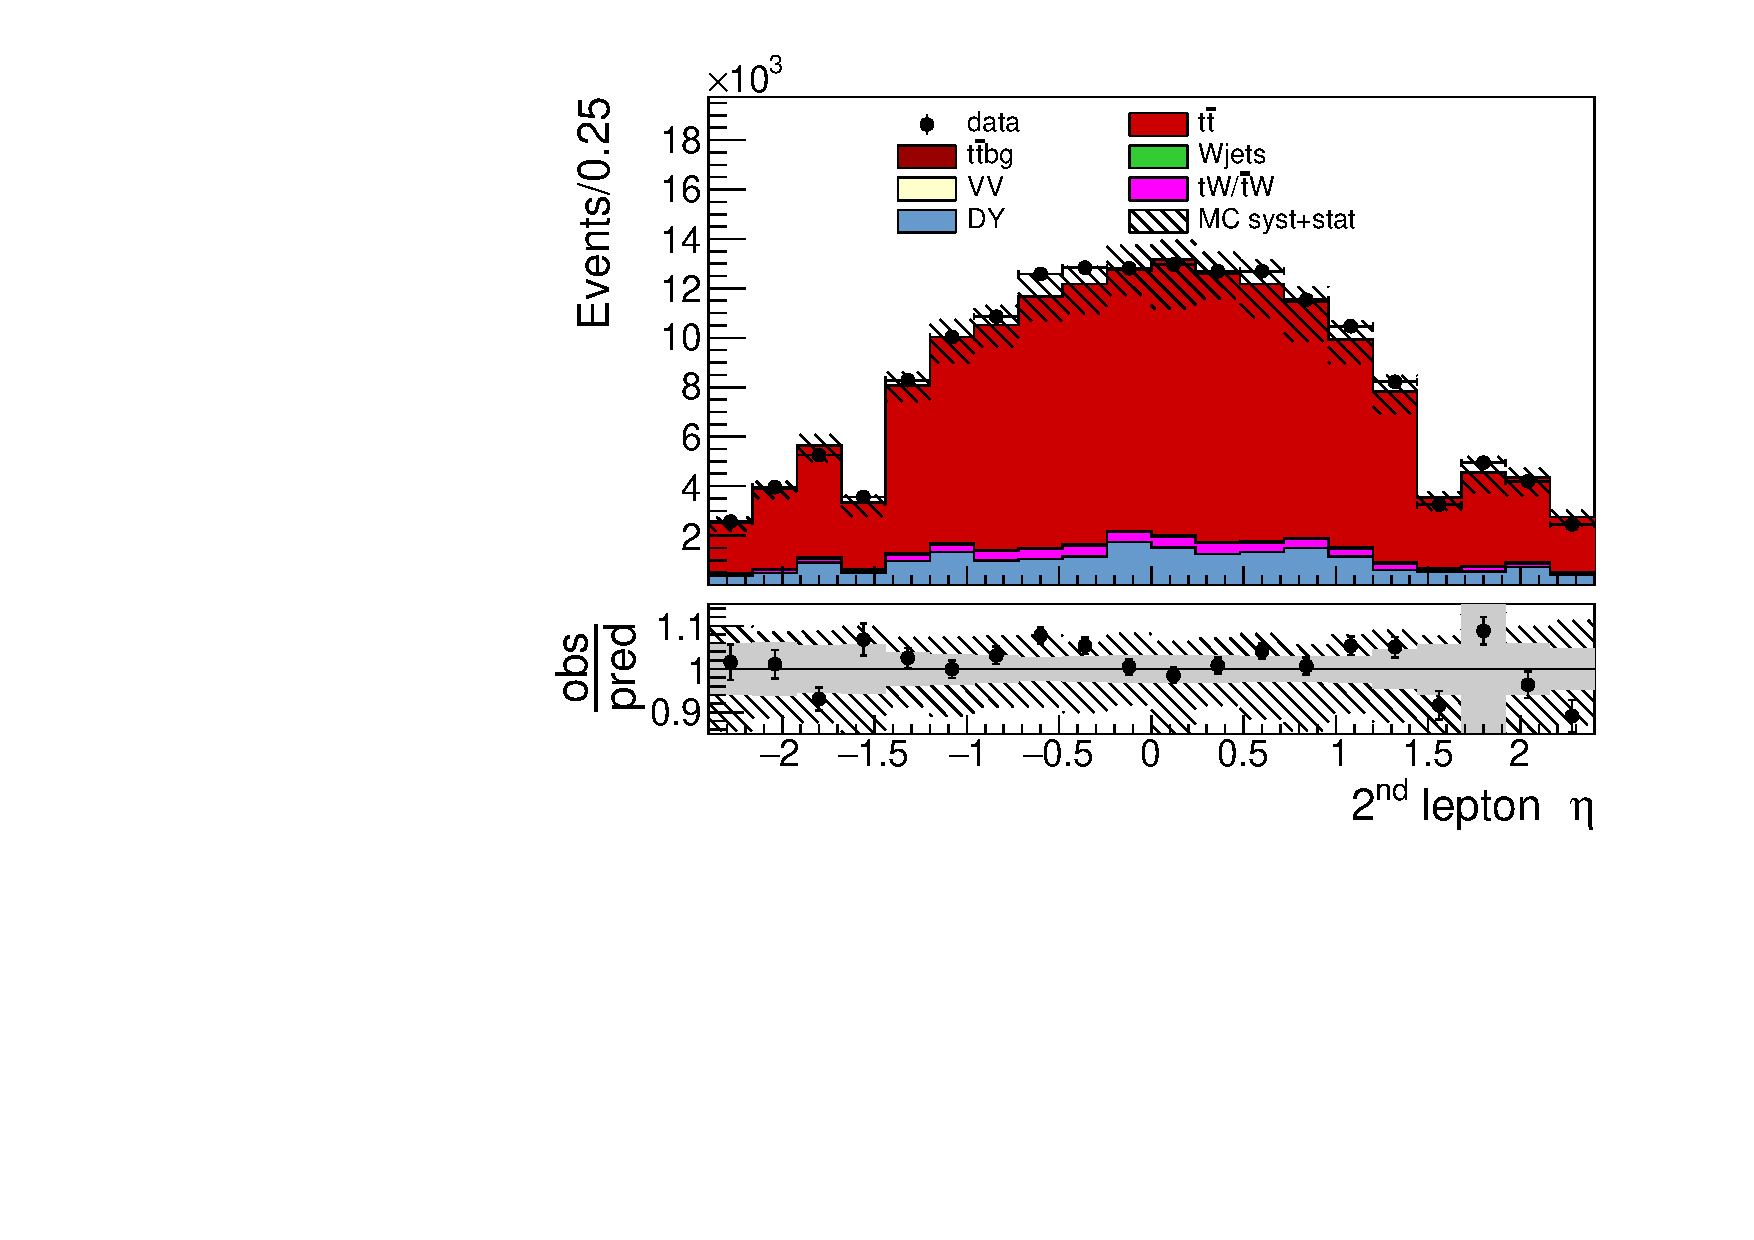
\includegraphics{CrossSection/Figures/ControlPlots/ee_sysnom/seclead_lepton_eta_step_8.pdf}}
    \resizebox{0.48 \textwidth}{!}{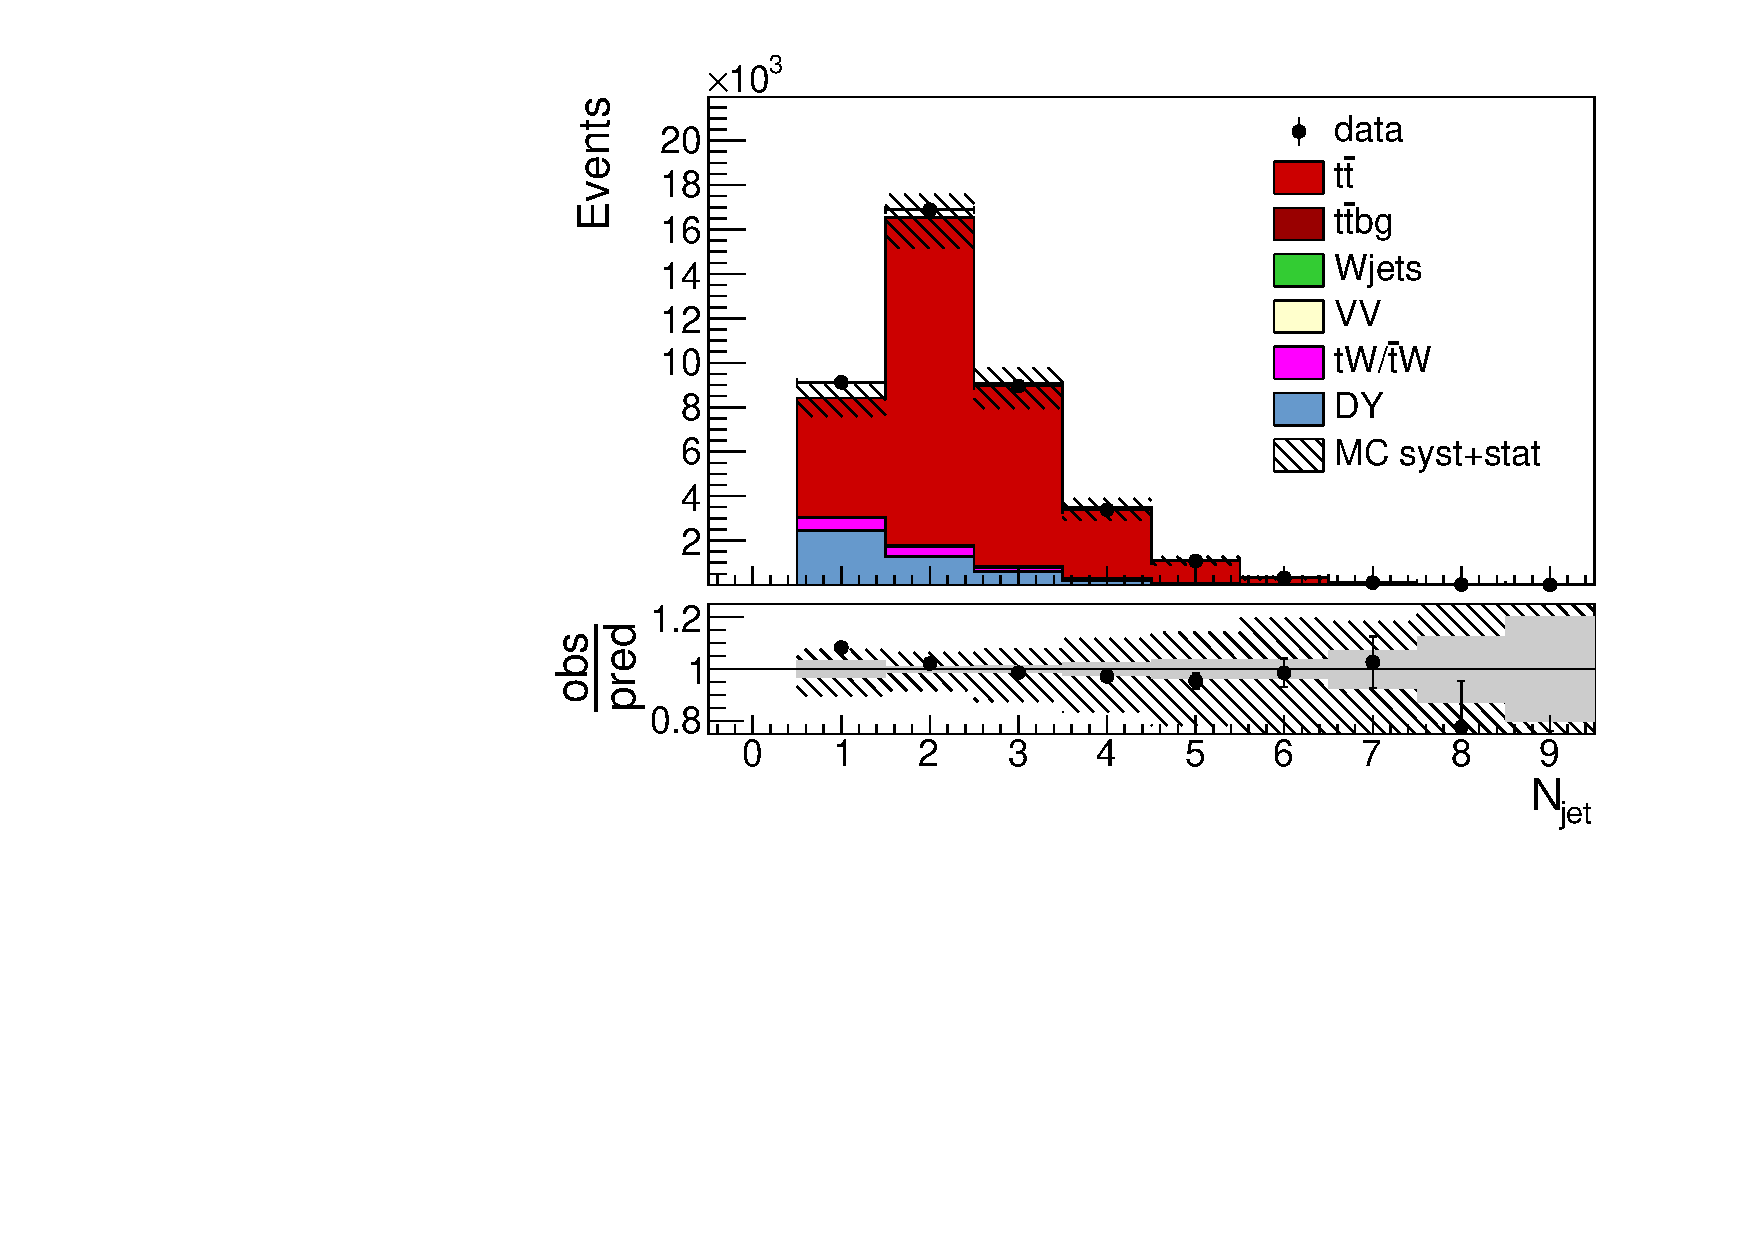
\includegraphics{CrossSection/Figures/ControlPlots/ee_sysnom/selected_jets_multi_step_8.pdf}}
    \resizebox{0.48 \textwidth}{!}{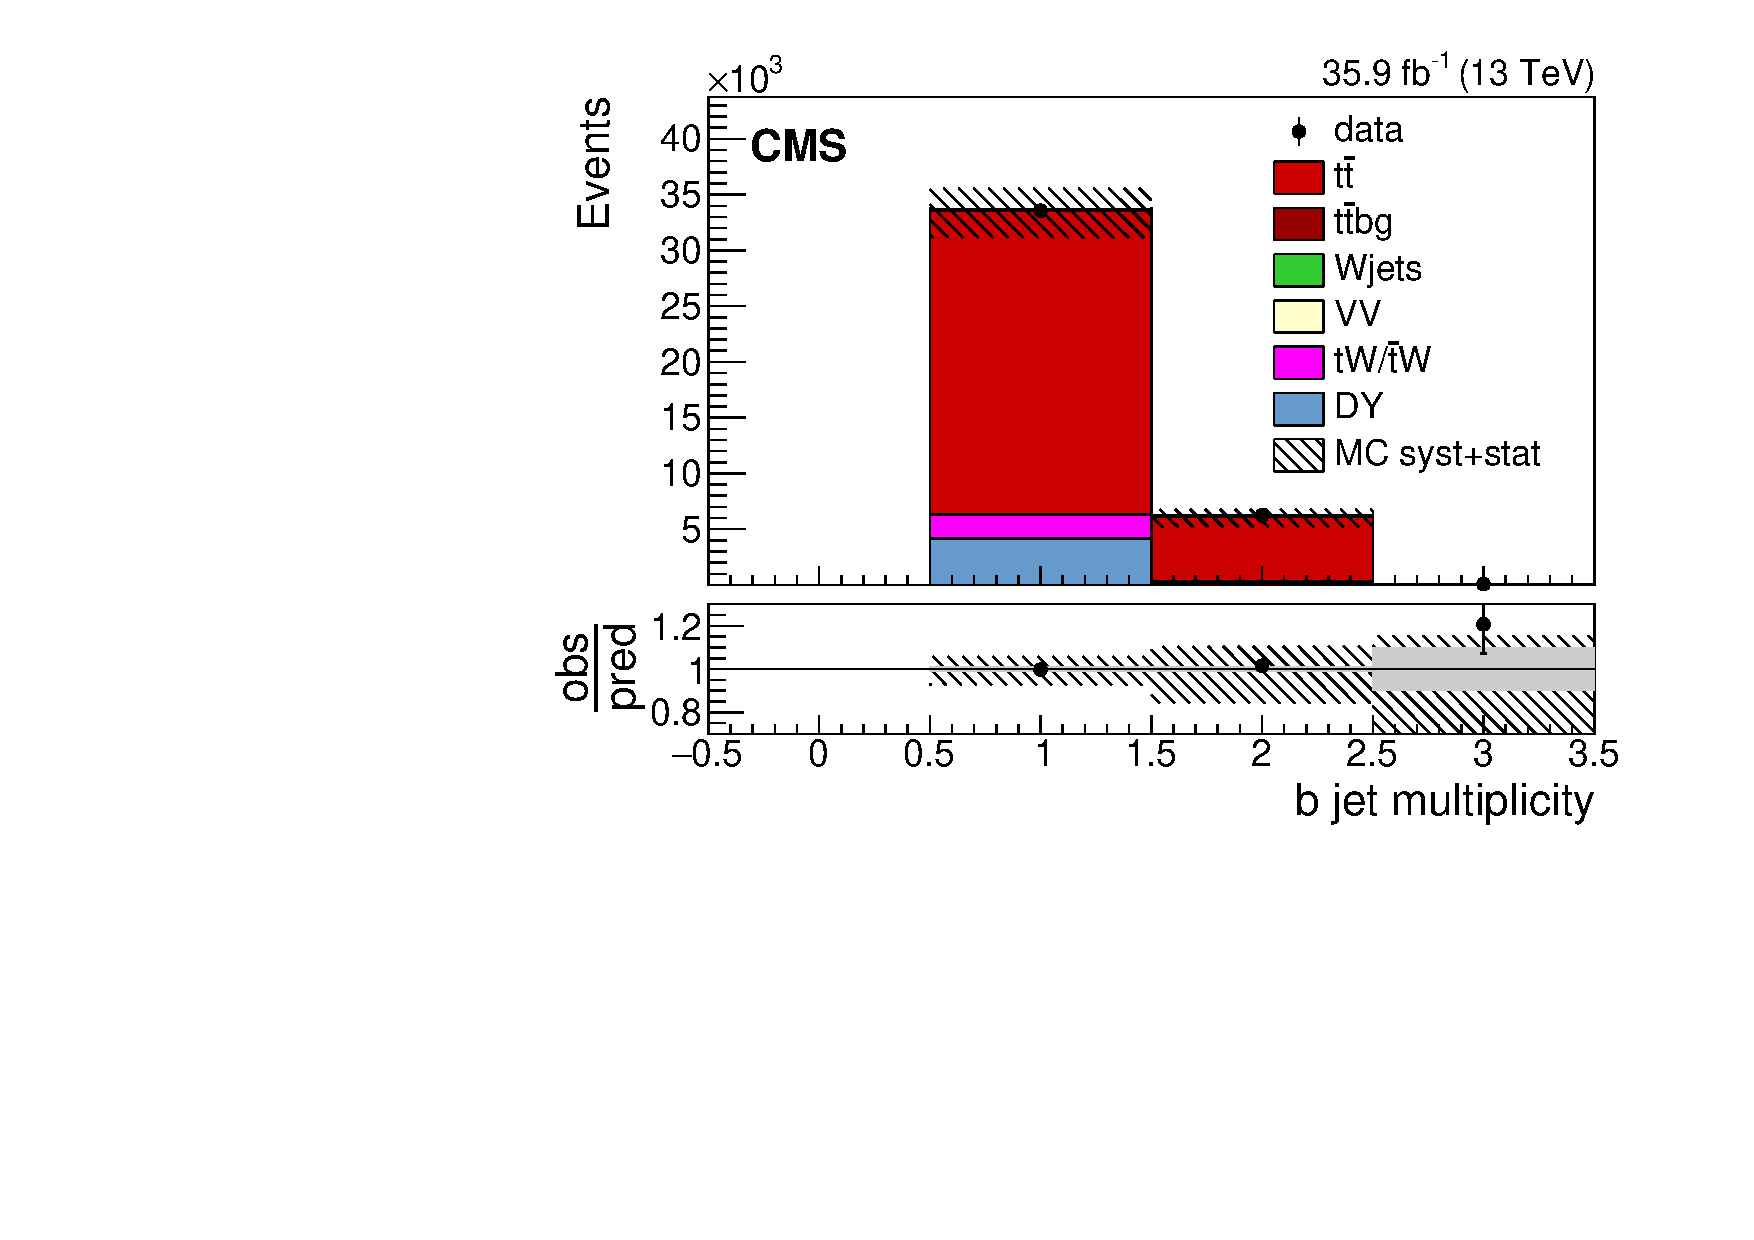
\includegraphics{CrossSection/Figures/ControlPlots/ee_sysnom/selected_b-jet_multi_step_8.pdf}}
      \caption{Transverse momentum (left) and pseudorapidity (right)
        of leading (first row) and second-leading (second row) lepton in the \ee channel after the
        event selection required by the \ttbar cross section
        extraction technique based on a simultaneous fit. Jet and b-jet multiplicity after the same selection steps are
        shown in the third row. The hatched
        bands correspond to the total uncertainty on the sum of the
        predicted yields. 
        %agrohsje , excluding luminosity and background
        %normalization uncertainties. 
        The ratios of data to the sum of the predicted yields are
        shown at the bottom of each plot. Here, the solid gray band
        represents the contribution of the statistical uncertainty.}  
       \label{fig:xsec_ee_ctrplots}
  \end{center}
\end{figure}

As described above, there are small differences between data and simulation, which are corrected in simulation based on independent measurements in data.
This is especially important for the leptons, as they define the phase space for this measurement.
In order to assess the quality of the correction a careful look into sensitive variables is important. Any large discrepancies between simulation and prediction would suggest that these corrections
are not optimal for the given selection.
The invariant mass of the dilepton system is shown in Figure \ref{fig:xsec_ctrplots_mll} for all three decay channels and depending on the number of b-tagged jets.
The simulation agrees with the measurement, so it can be assumed that the efficiency corrections are accurate.
The figures also show again how the DY contribution decreases when more b-tagged jets are required.


\begin{figure}[htbp!]
  \begin{center}
    \resizebox{0.48 \textwidth}{!}{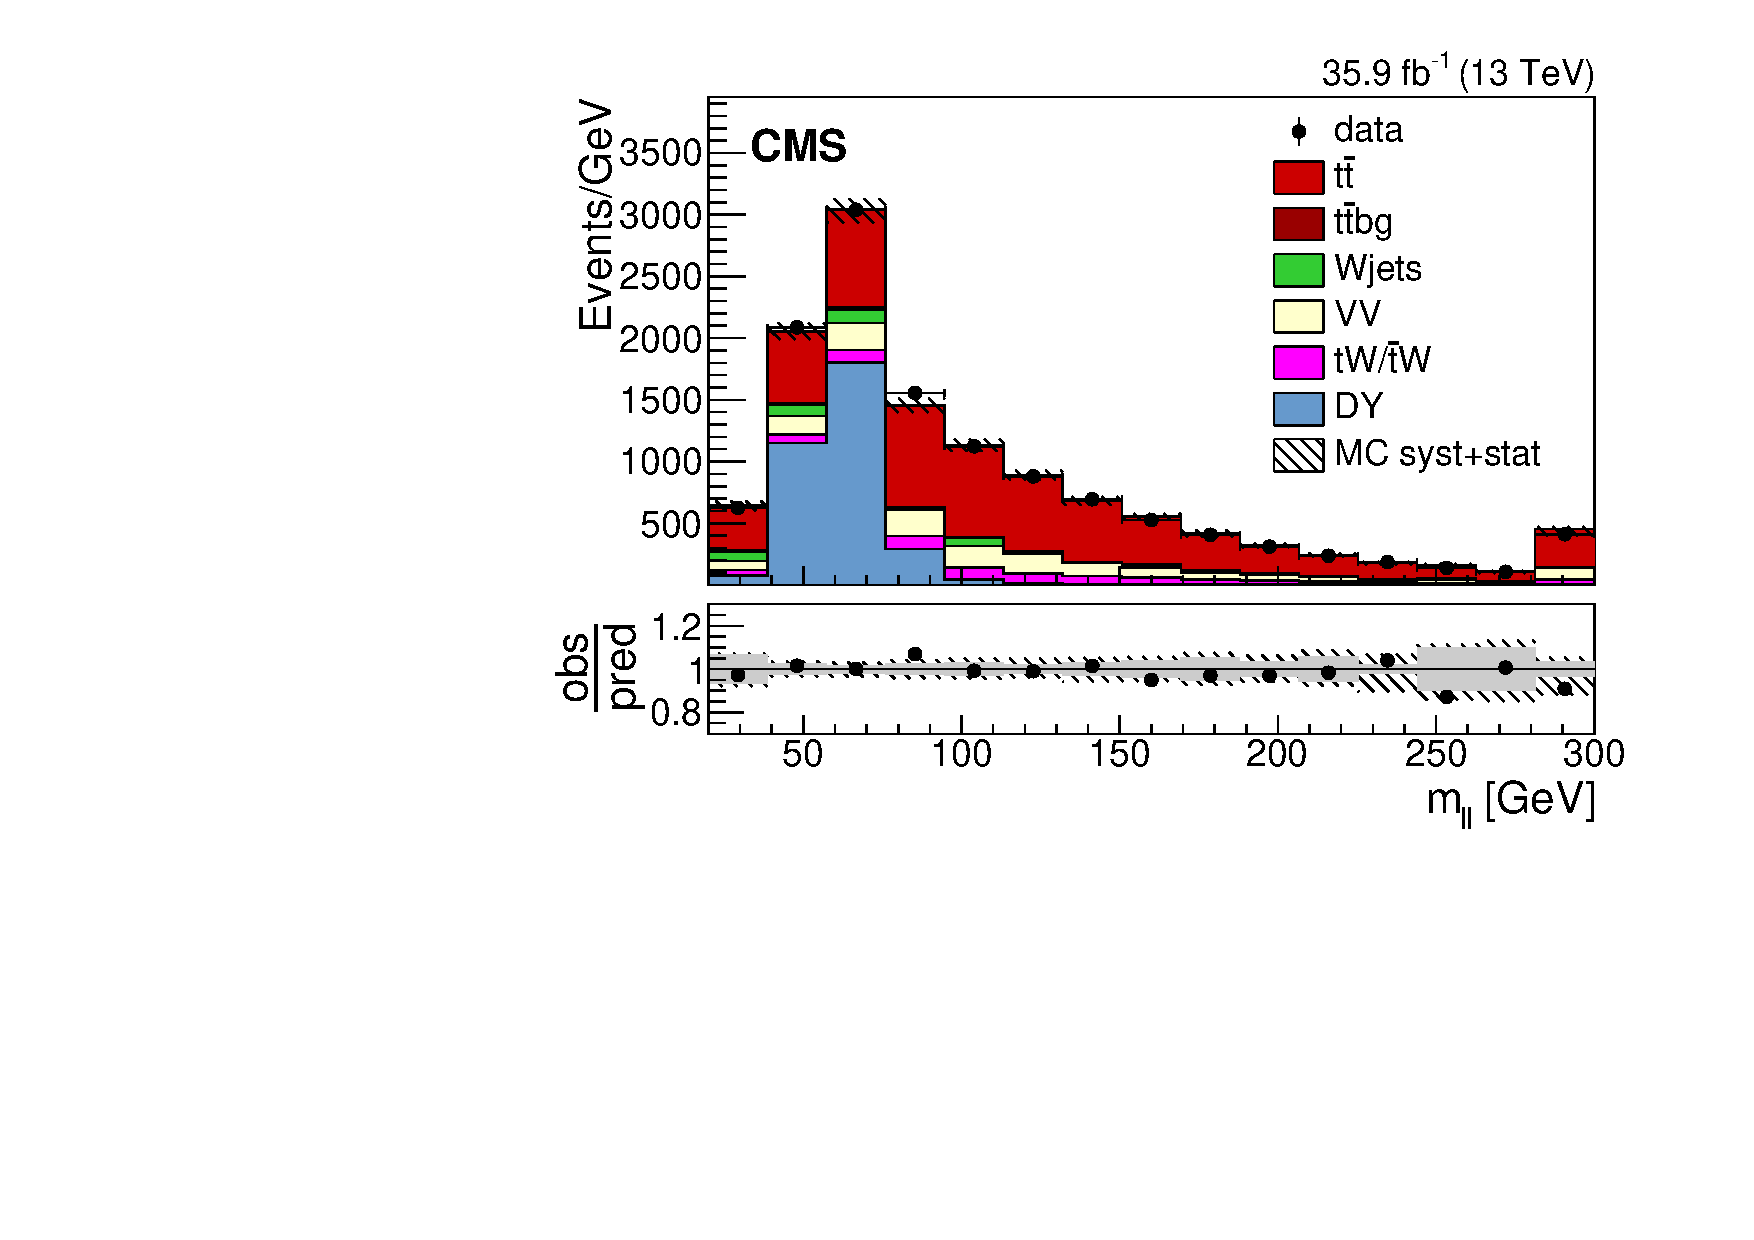
\includegraphics{CrossSection/Figures/ControlPlots/emu_sysnom/mll_0_b-jets_step_8.pdf}}
    \resizebox{0.48 \textwidth}{!}{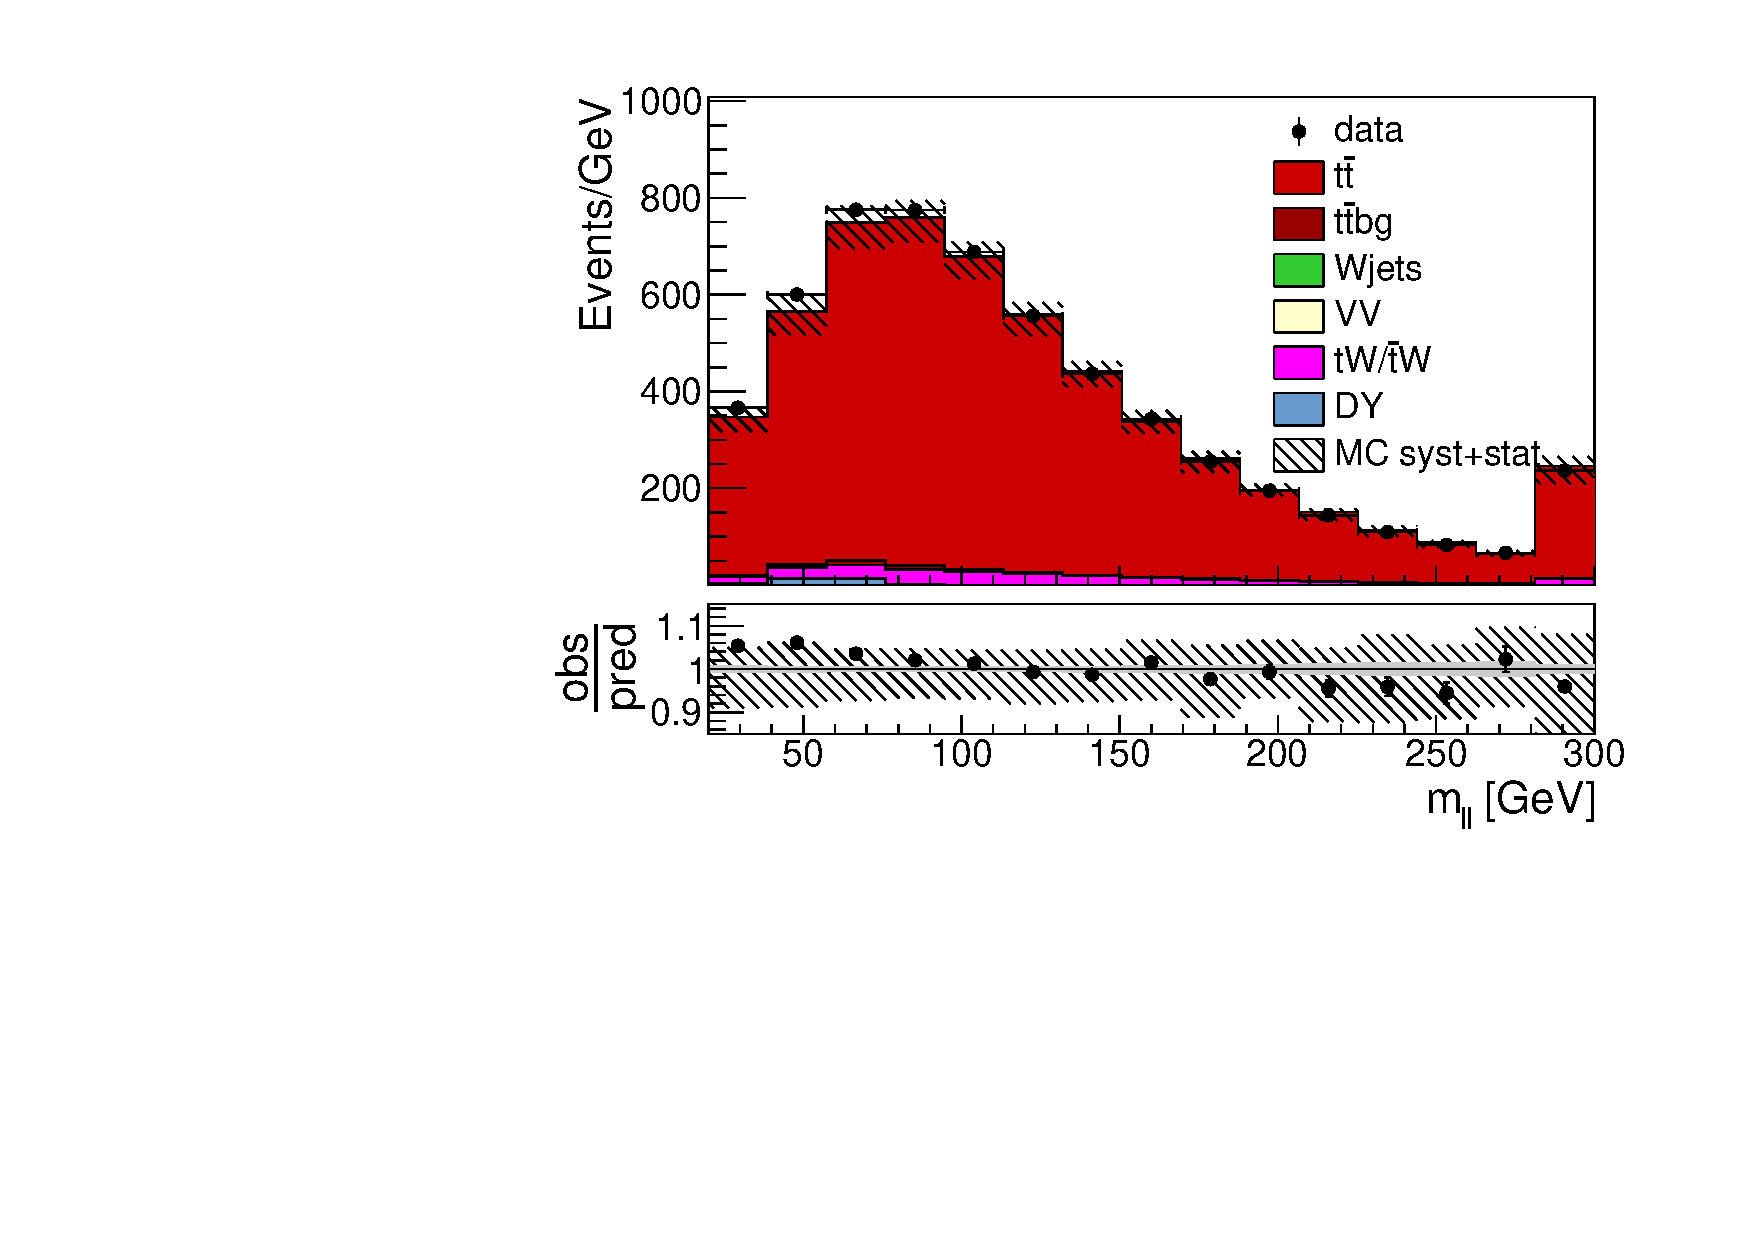
\includegraphics{CrossSection/Figures/ControlPlots/emu_sysnom/mll_1_b-jets_step_8.pdf}}
    \resizebox{0.48 \textwidth}{!}{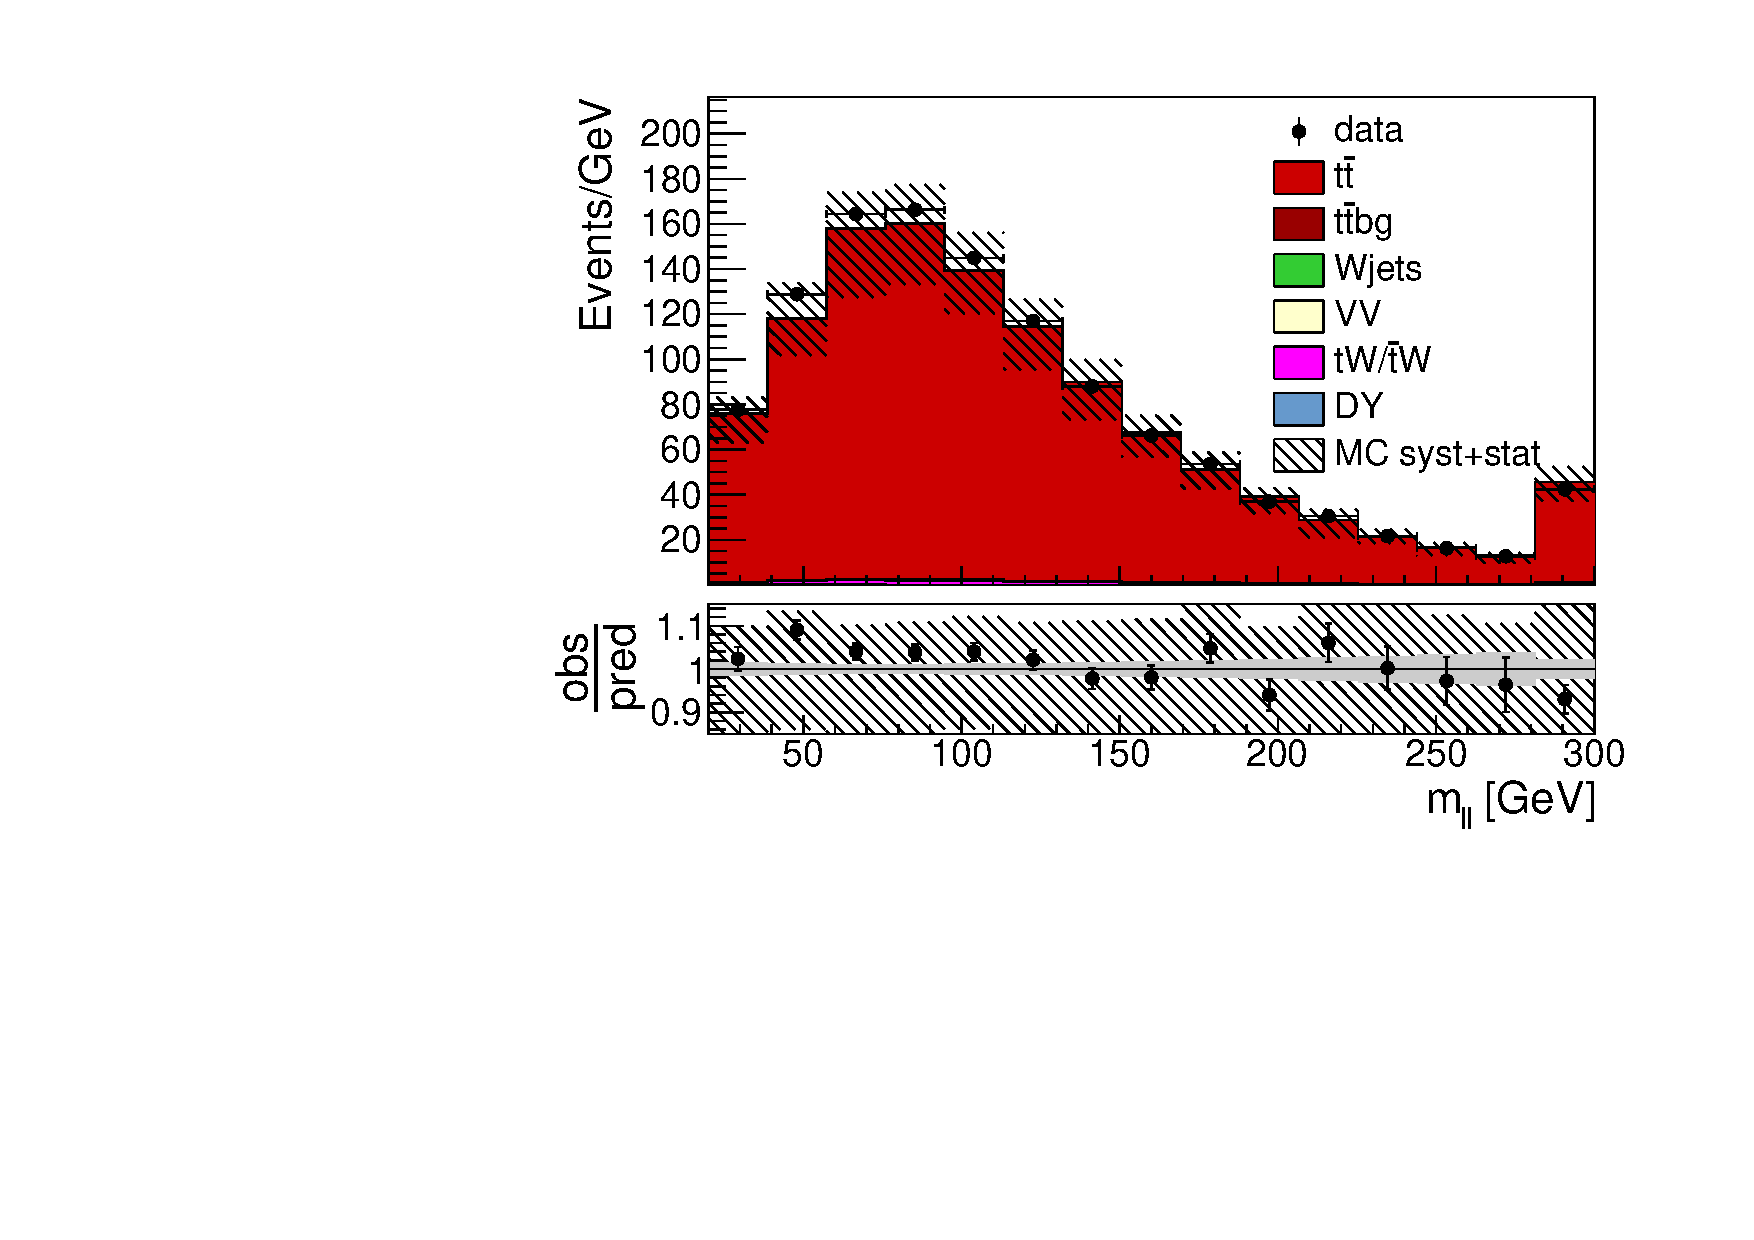
\includegraphics{CrossSection/Figures/ControlPlots/emu_sysnom/mll_2_b-jets_step_8.pdf}} \\
        \resizebox{0.48 \textwidth}{!}{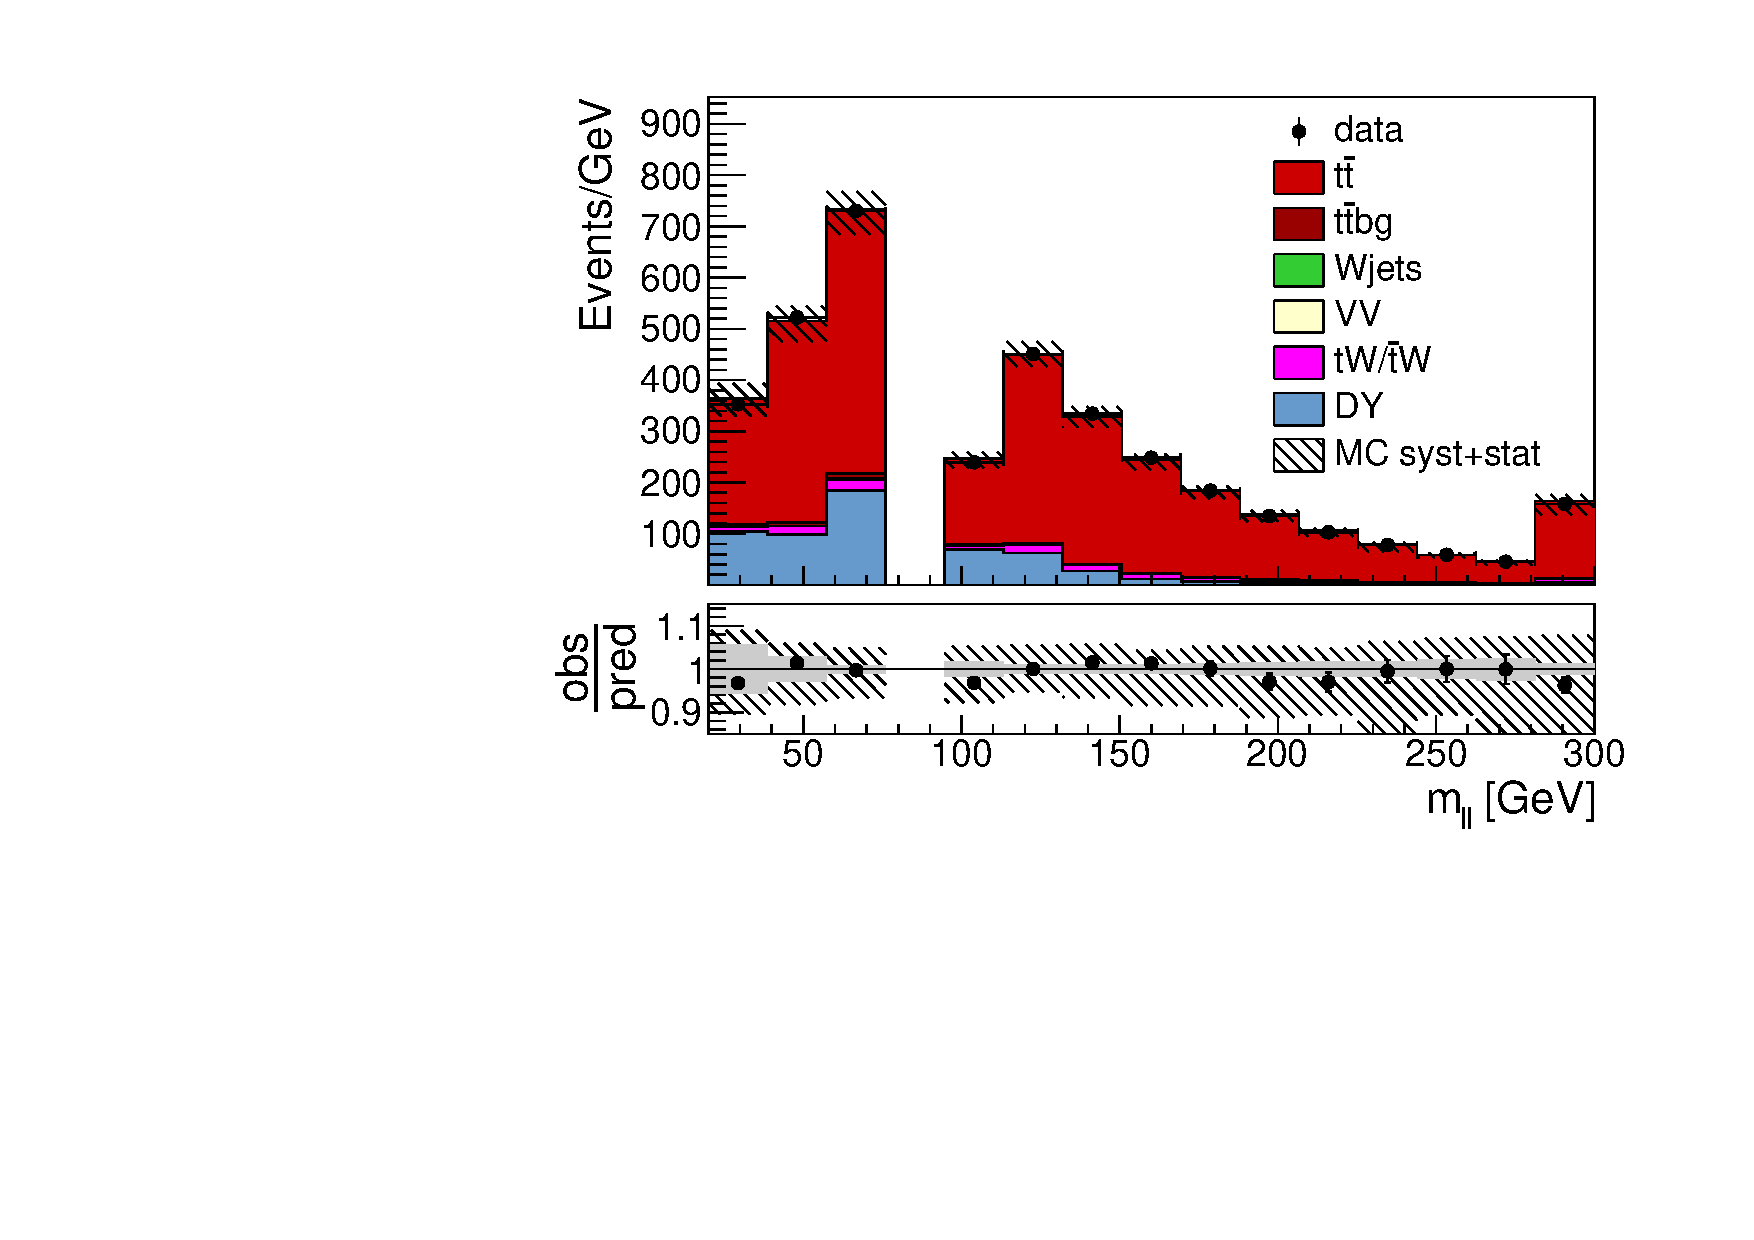
\includegraphics{CrossSection/Figures/ControlPlots/mumu_sysnom/mll_1_b-jets_step_8.pdf}}
    \resizebox{0.48 \textwidth}{!}{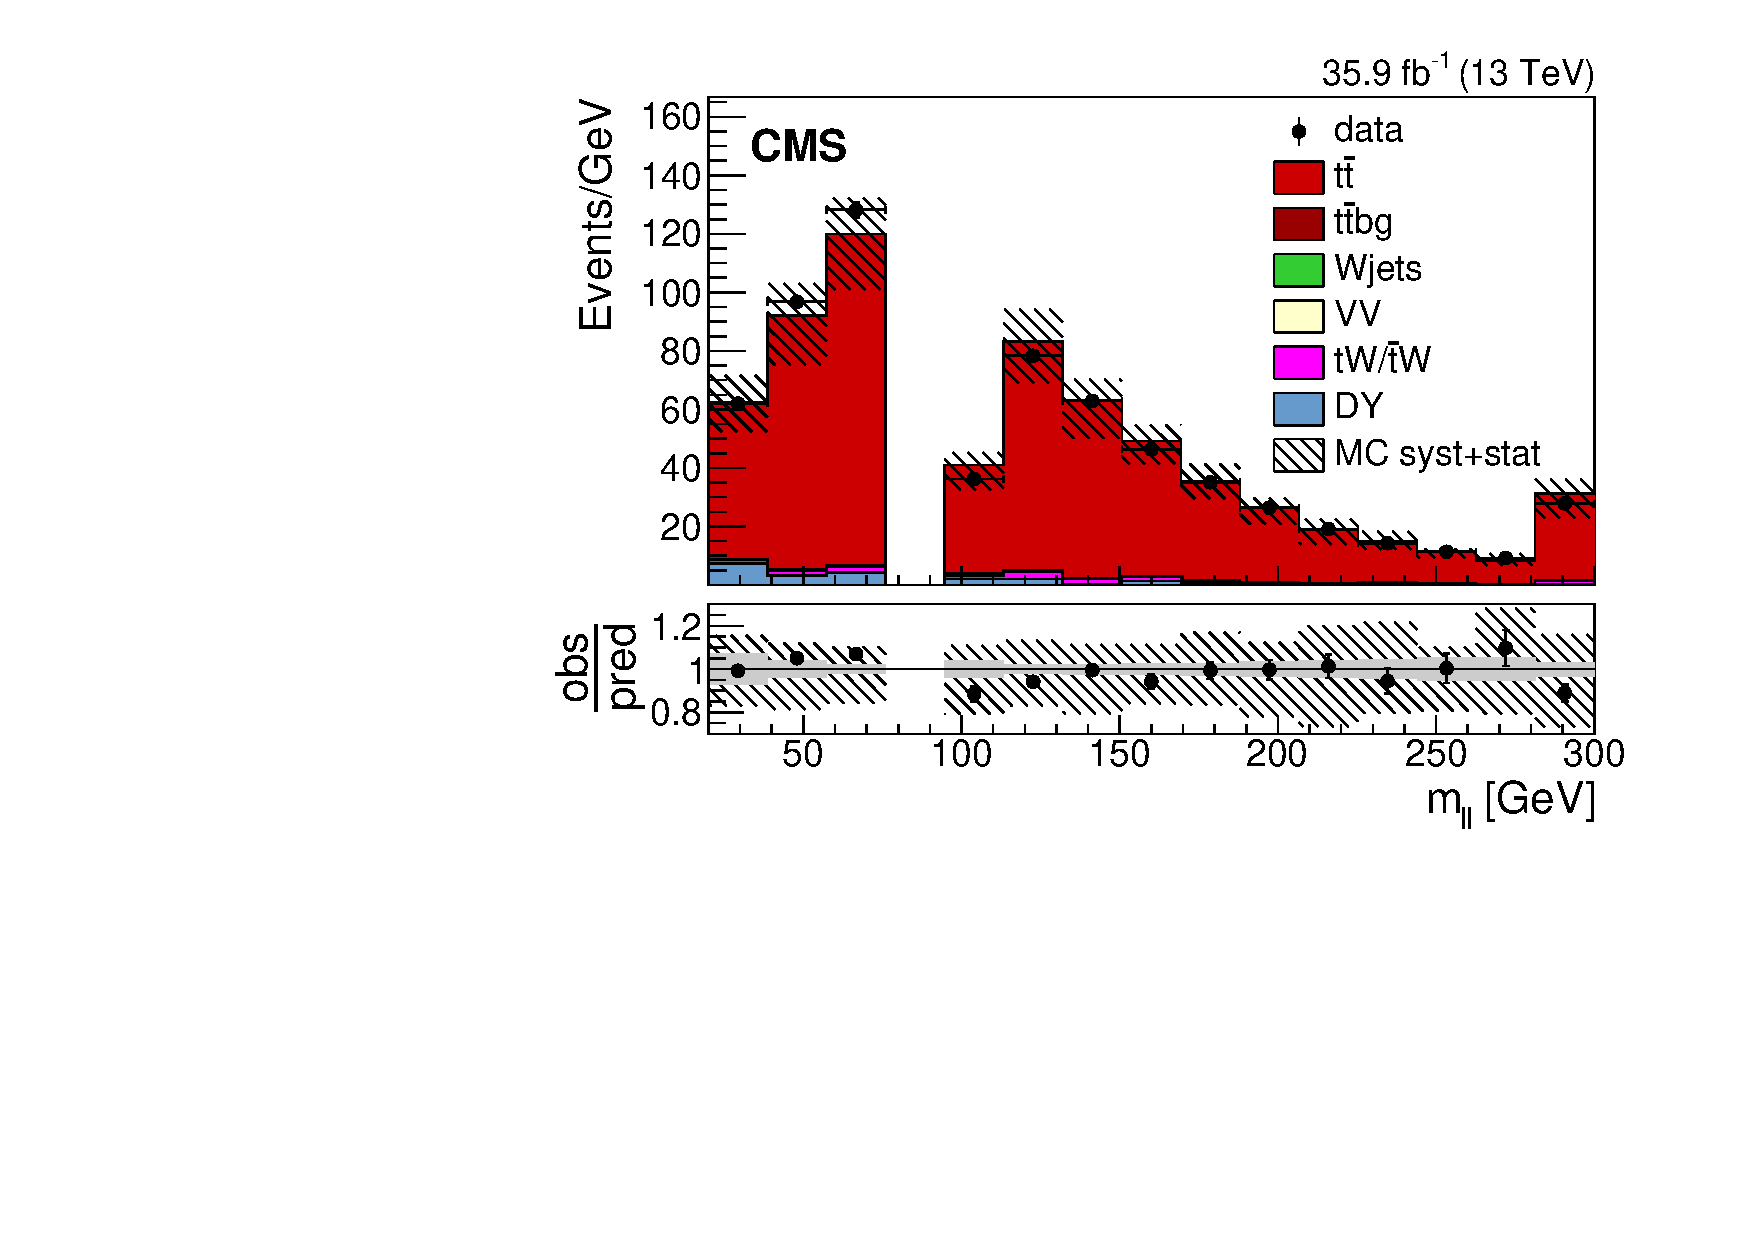
\includegraphics{CrossSection/Figures/ControlPlots/mumu_sysnom/mll_2_b-jets_step_8.pdf}} \\
        \resizebox{0.48 \textwidth}{!}{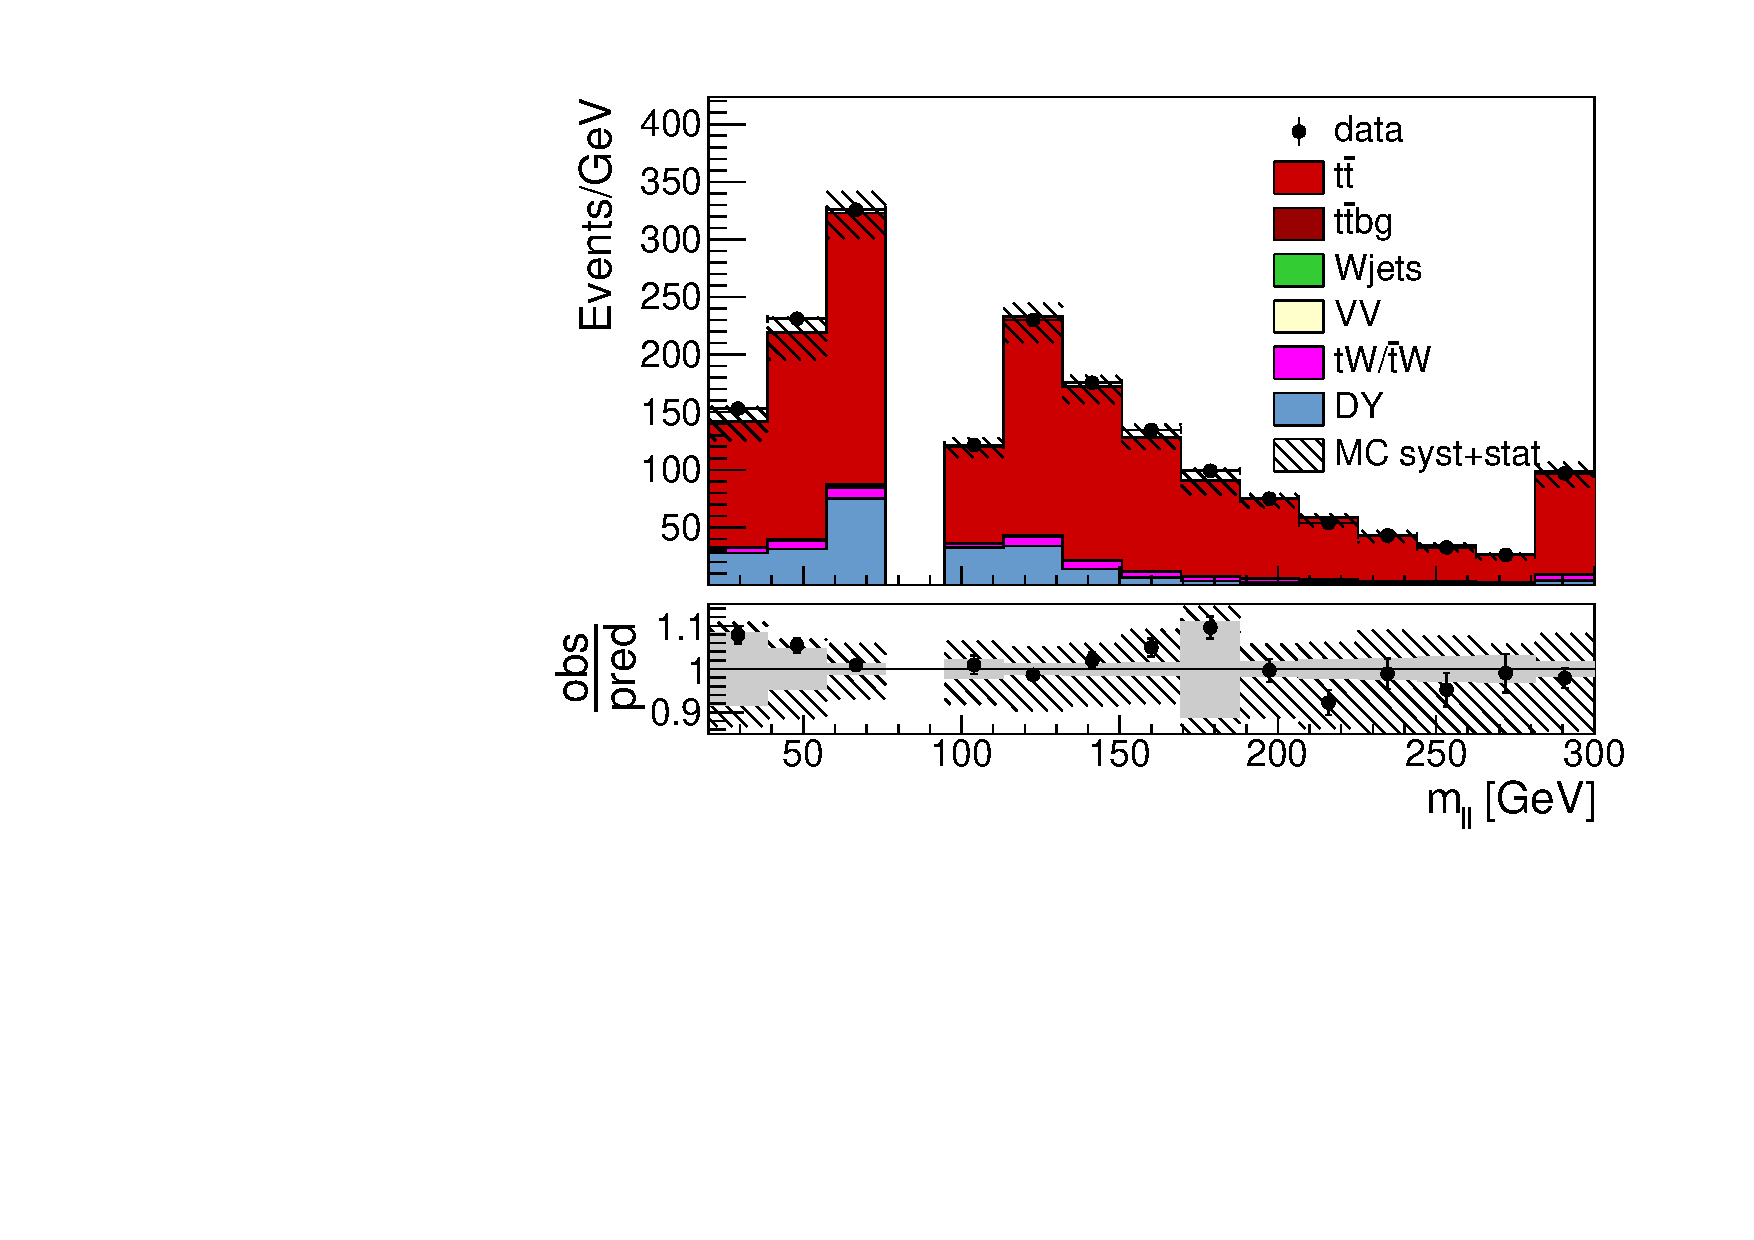
\includegraphics{CrossSection/Figures/ControlPlots/ee_sysnom/mll_1_b-jets_step_8.pdf}}
    \resizebox{0.48 \textwidth}{!}{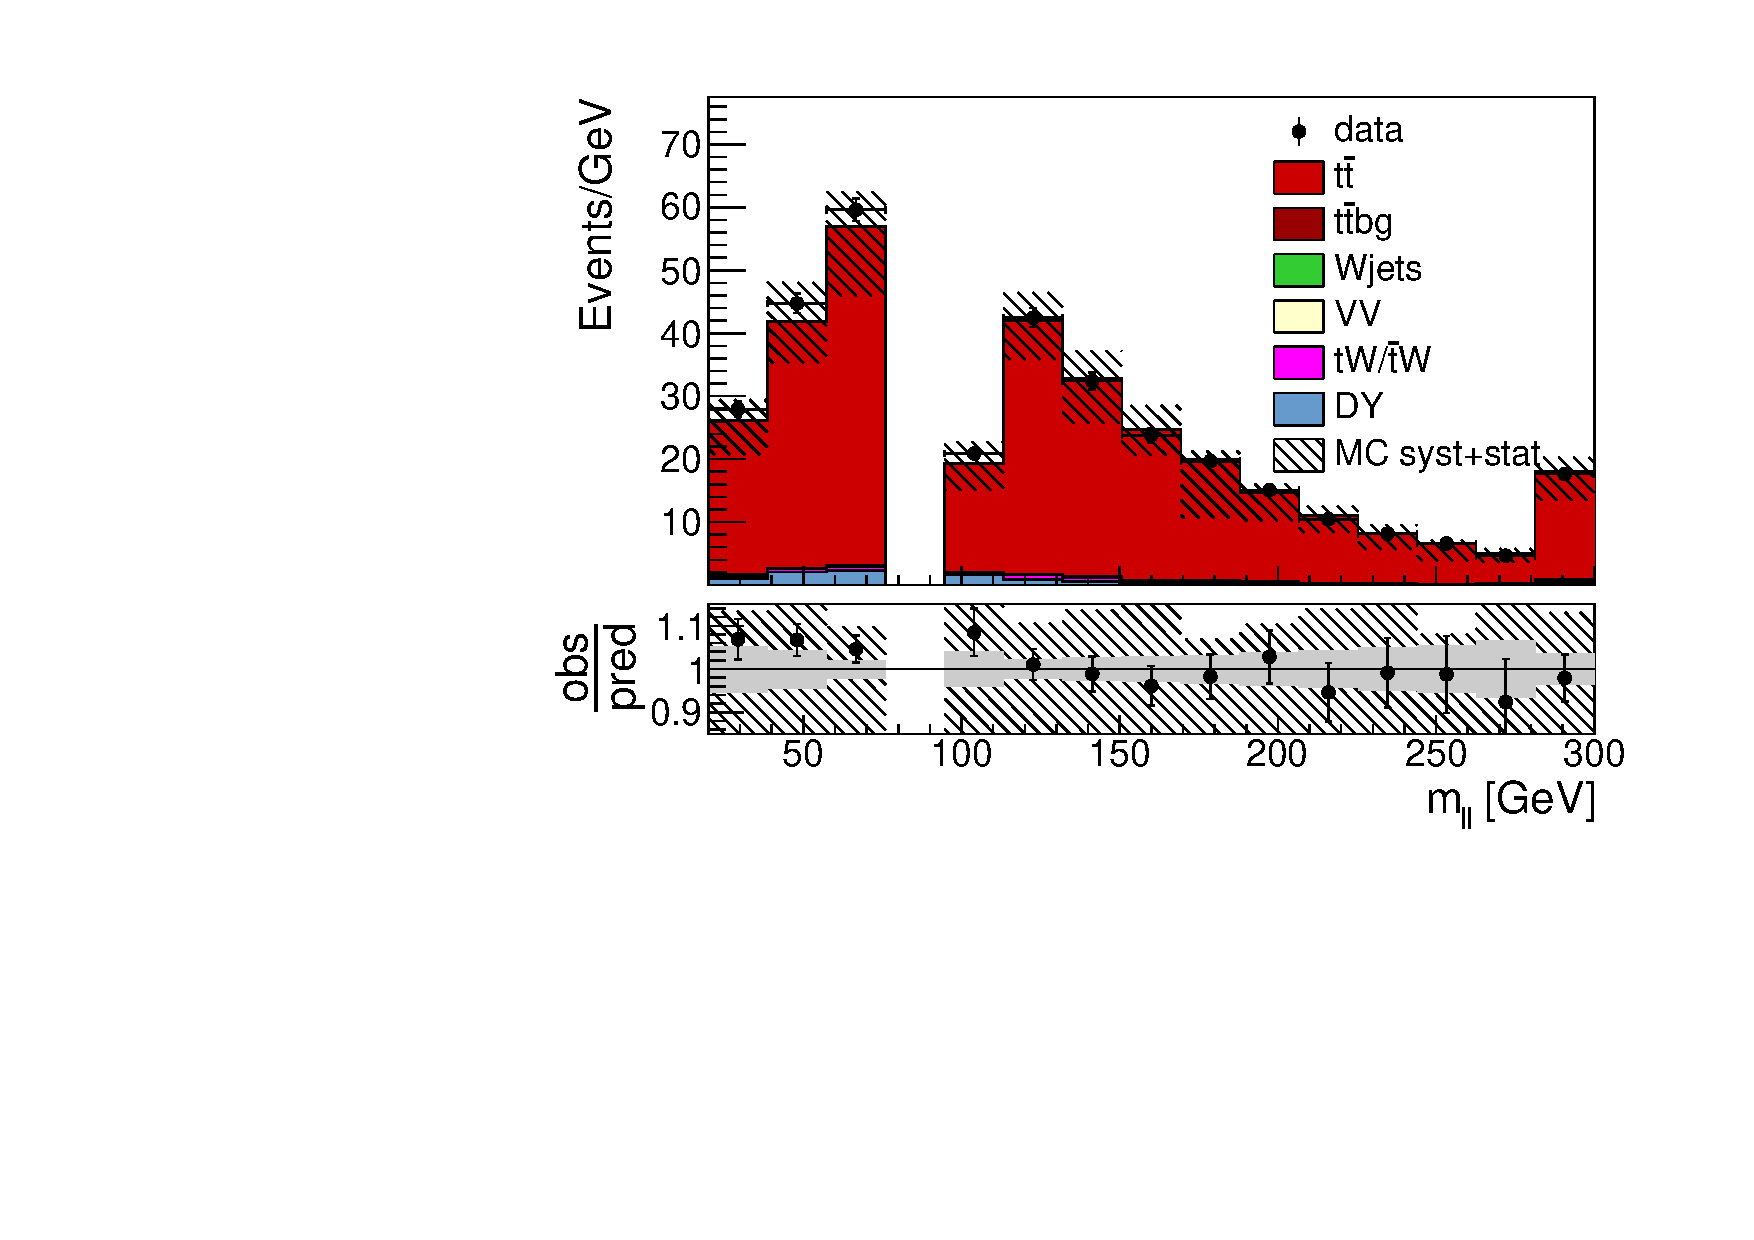
\includegraphics{CrossSection/Figures/ControlPlots/ee_sysnom/mll_2_b-jets_step_8.pdf}}

      \caption{Invariant mass of the dilepton system with zero (top row left), one (top row right) and two (second row) b-tagged 
      jets in the \emu channel. The invariant mass of the dilepton system in the \mumu (third row) and \ee (bottom row) with one (left)
      and two b-tagged jets (right).
        %agrohsje , excluding luminosity and background
        %normalization uncertainties. 
        The ratios of data to the sum of the predicted yields are
        shown at the bottom of each plot. Here, the solid gray band
        represents the contribution of the statistical uncertainty.}  
       \label{fig:xsec_ctrplots_mll}
  \end{center}
\end{figure}



\section{Choice of Event Categories and Template Distributions}
\label{sec:xsec_templates}


In order to increase the separation between signal and background the events are divided according to the number of b-tagged jets.
There are three categories of events with one, two and zero or more than two b-tagged jets.
This further categorisation also allows to determine the efficiency to find a b-tagged jet in a signal event using the topology of \ttbar decays.
Since each of the top quarks decays into a W boson and a b quark it can be assumed that every \ttbar event should contain two jets originating from a b quark.
Any decays of a top quark to a W boson and a light quark can be considered negligible.
It can therefore be assumed that selecting less than two b-tagged jets in a \ttbar event is a measure for the inefficiency of the selection of b-tagged jets.

Treating the b-tagging efficiency in this way allows the explicit and independent determination of the b-tagging efficiency for data and simulation depending on the nuisance parameters. The efficiency of the b-tagging algorithm is independent of the rest of the event, so it can be assumed to be the same in all \ttbar decay channels.
This intrinsic measurement of the b-tagging efficiency in the phase space of the measurement is also expected to reduce the impact of the uncertainties on the b-tagging efficiency on the final measurement of the \ttbar cross section.

Beside the number of b-jets, the number of light (non b-tagged) jets is one of the main discriminators between \ttbar and background events.
\ttbar events tend to have a higher amount of additional jets from final state radiation, especially when compared with Drell-Yan events.
Events are split according to the number of light jets from 0 to 3 or more.
For the actual template distributions the \pt of the trailing light jet is chosen.
Together with the \pt of the light jets their multiplicity is sensitive to the systematic uncertainty on the response of the jet reconstruction and
the systematic uncertainties introduced by theoretical assumptions in the simulation.

The separation of events according to the decay channel is given by the selection. The \ttbar production cross section does not depend on the decay, which introduces a correlation for all three channels.
By simultaneously fitting the three channels(\emu, \ee, \mumu) the two uncorrelated single-lepton identification efficiencies $\epsilon_e$ and $\epsilon_\mu$ are constrained against one another. 
These constraints can be illustrated by considering the correlation between the number of events in each dilepton channel ($s_{\emu}$, $s_{ee}$ and $s_{\mu\mu}$), the ttbar cross section (\stt) and the lepton 
efficiencies, that is shown in simplified form in Equation \ref{eq:xsec_lepsplit}.
\begin{eqnarray}
s_{\emu}  &\propto& \stt \epsilon_{e} \epsilon_{\mu}  \\
s_{\ee}  &\propto&  \stt \epsilon_{e}^2  \\
s_{\mumu}  &\propto&  \stt \epsilon_{\mu}^2
\label{eq:xsec_lepsplit}.
\end{eqnarray}
Using the number of events in the \emu channel these relations can be broken down, as shown in Equation \ref{eq:xsec_lepeffs}.

\begin{equation}
\frac{s_{\mu\mu}}{s_{ee}} = \frac{\epsilon_{\mu}^2}{\epsilon_{e}^2}
\label{eq:xsec_lepeffs}
\end{equation}

The number of events in each channels is known within uncertainties, so the ratio of the lepton efficiencies can implicitely be constrained in the fit.
Here, prior to the fit, the muon identification uncertainty is smaller, and thus in the fit the single-electron identification uncertainty is constrained to that of the muon.



In summary events are divided by the dilepton decay channel into the \emu, \ee and \mumu categories. Following that they are separated according to the number of b-tagged jets into events with one, two and zero or more b-tagged jets. For the same flavour channels (\ee, \mumu) only events with more than one b-tagged jet are considered. The resulting seven categories are further subdivided according to the number of additional jets (not b-tagged) into events with zero,one,two or three or more additional jets. The final 28 templates are shown in Figures 
 \ref{fig:xsec_emu_inputdistr}, \ref{fig:xsec_mumu_inputdistr} and \ref{fig:xsec_ee_inputdistr} for the \emu, \mumu and \ee channel respectively.

\begin{figure}[htbp!]
  \begin{center}
    \resizebox{0.32 \textwidth}{!}{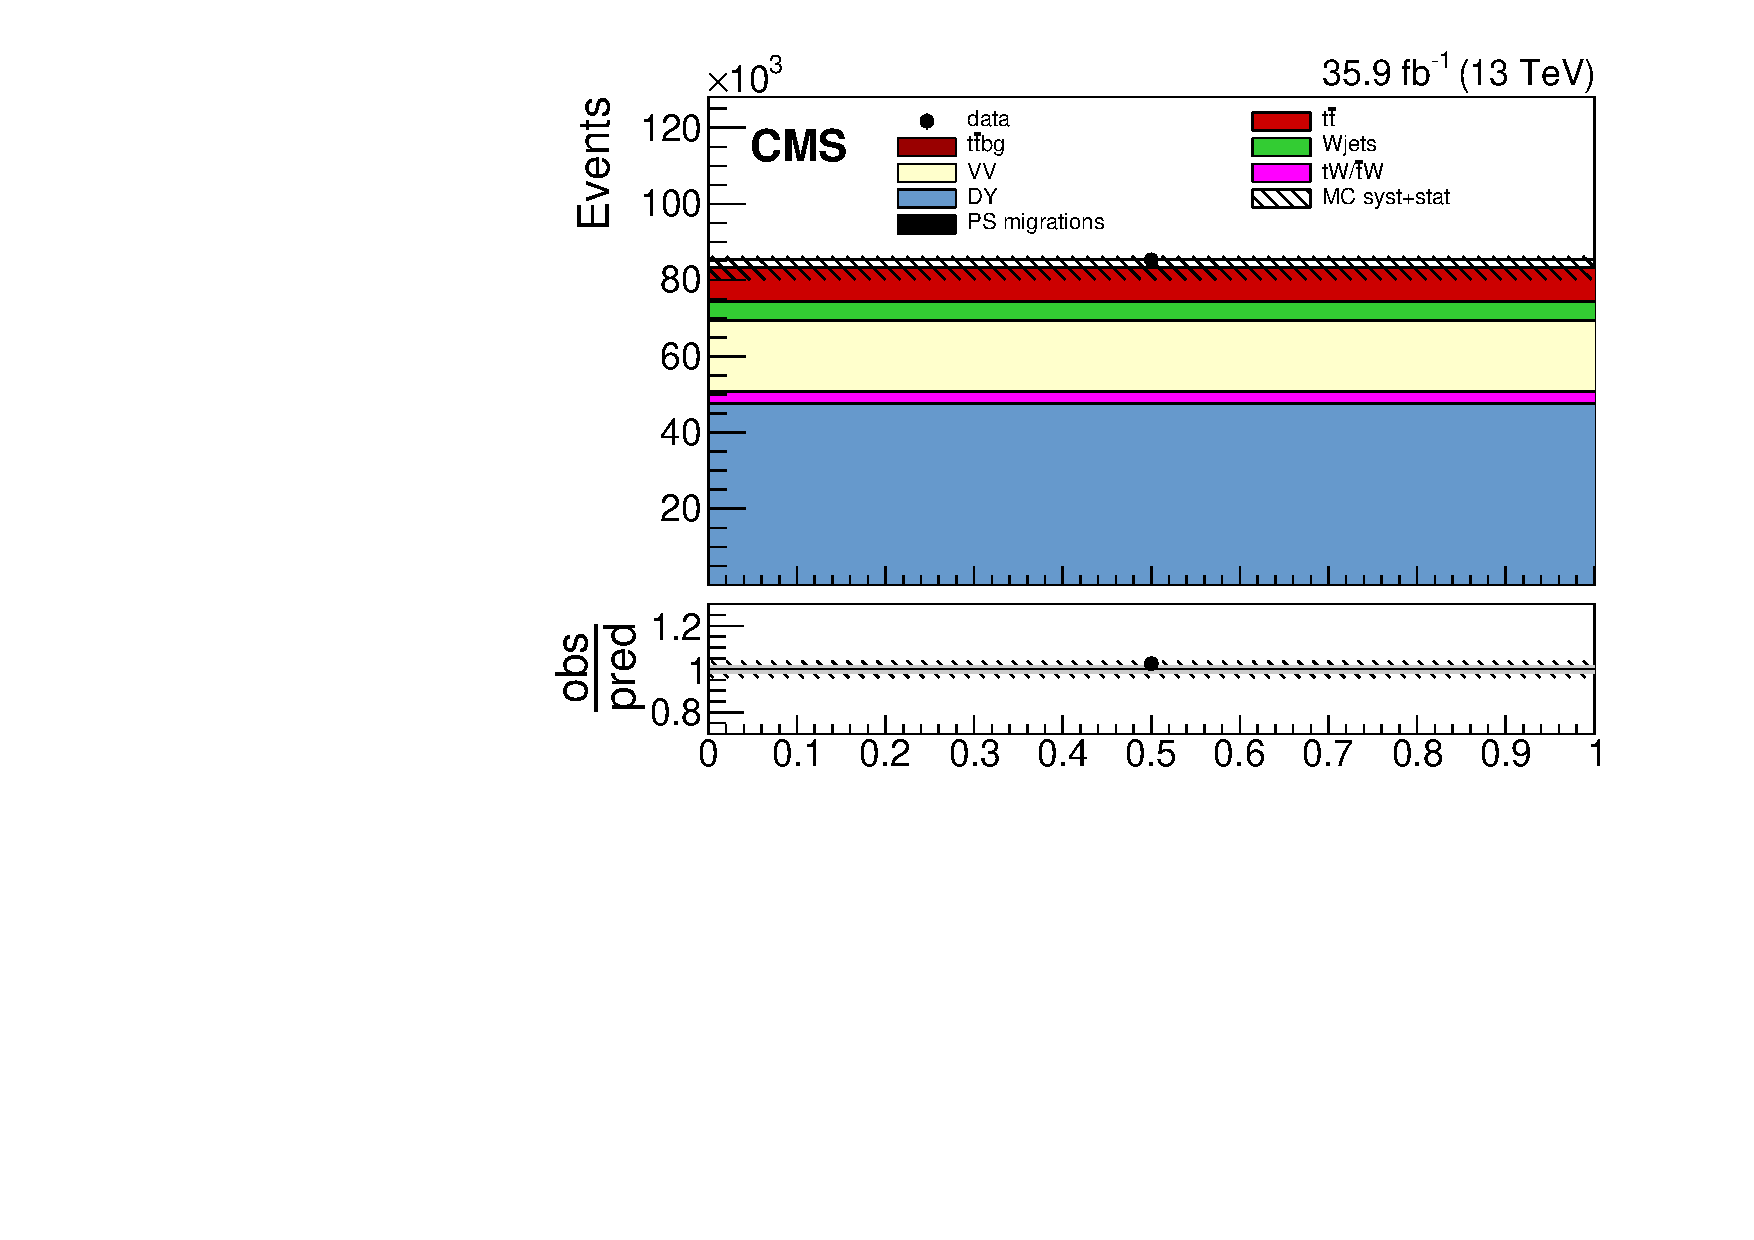
\includegraphics{CrossSection/Figures/ControlPlots/emu_sysnom/total_0_0_b-jets_step_8.pdf}}
    \resizebox{0.32 \textwidth}{!}{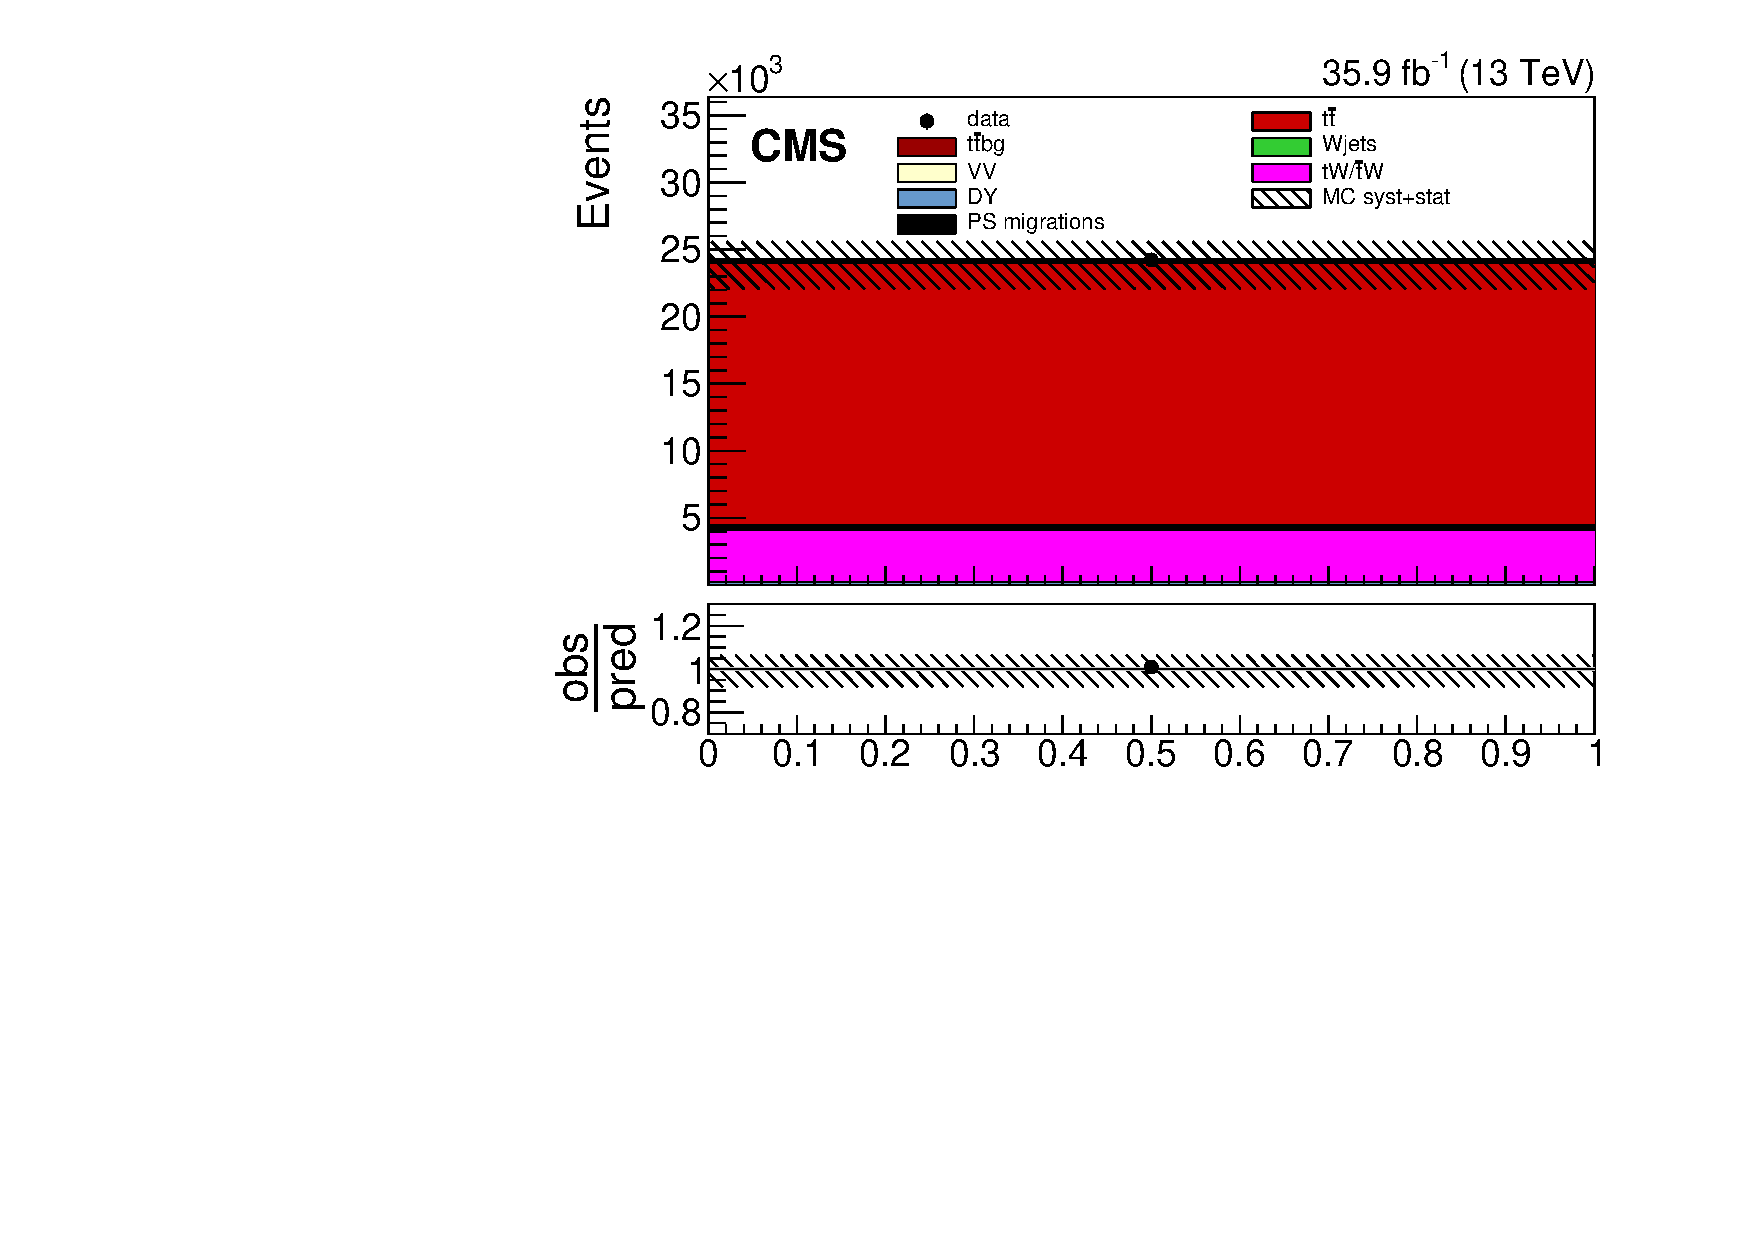
\includegraphics{CrossSection/Figures/ControlPlots/emu_sysnom/total_1_0_b-jets_step_8.pdf}}
    \resizebox{0.32 \textwidth}{!}{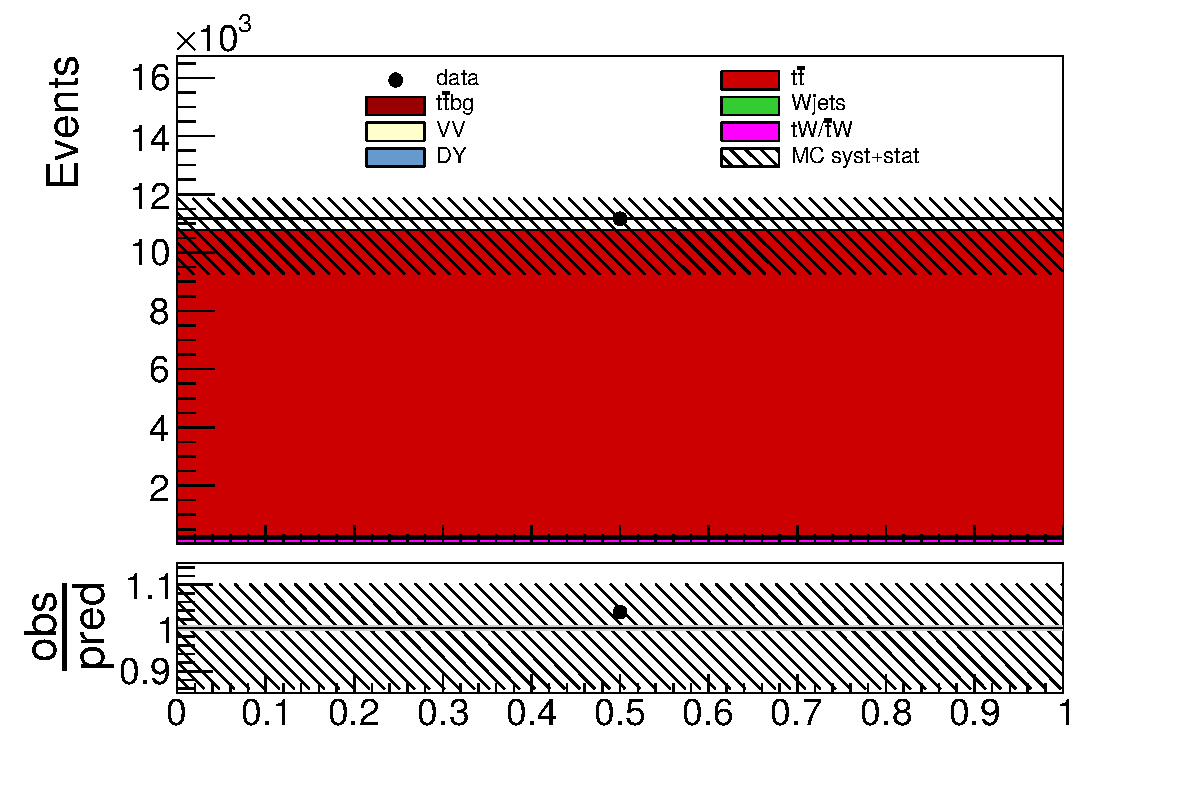
\includegraphics{CrossSection/Figures/ControlPlots/emu_sysnom/total_2_0_b-jets_step_8.pdf}}

    \resizebox{0.32 \textwidth}{!}{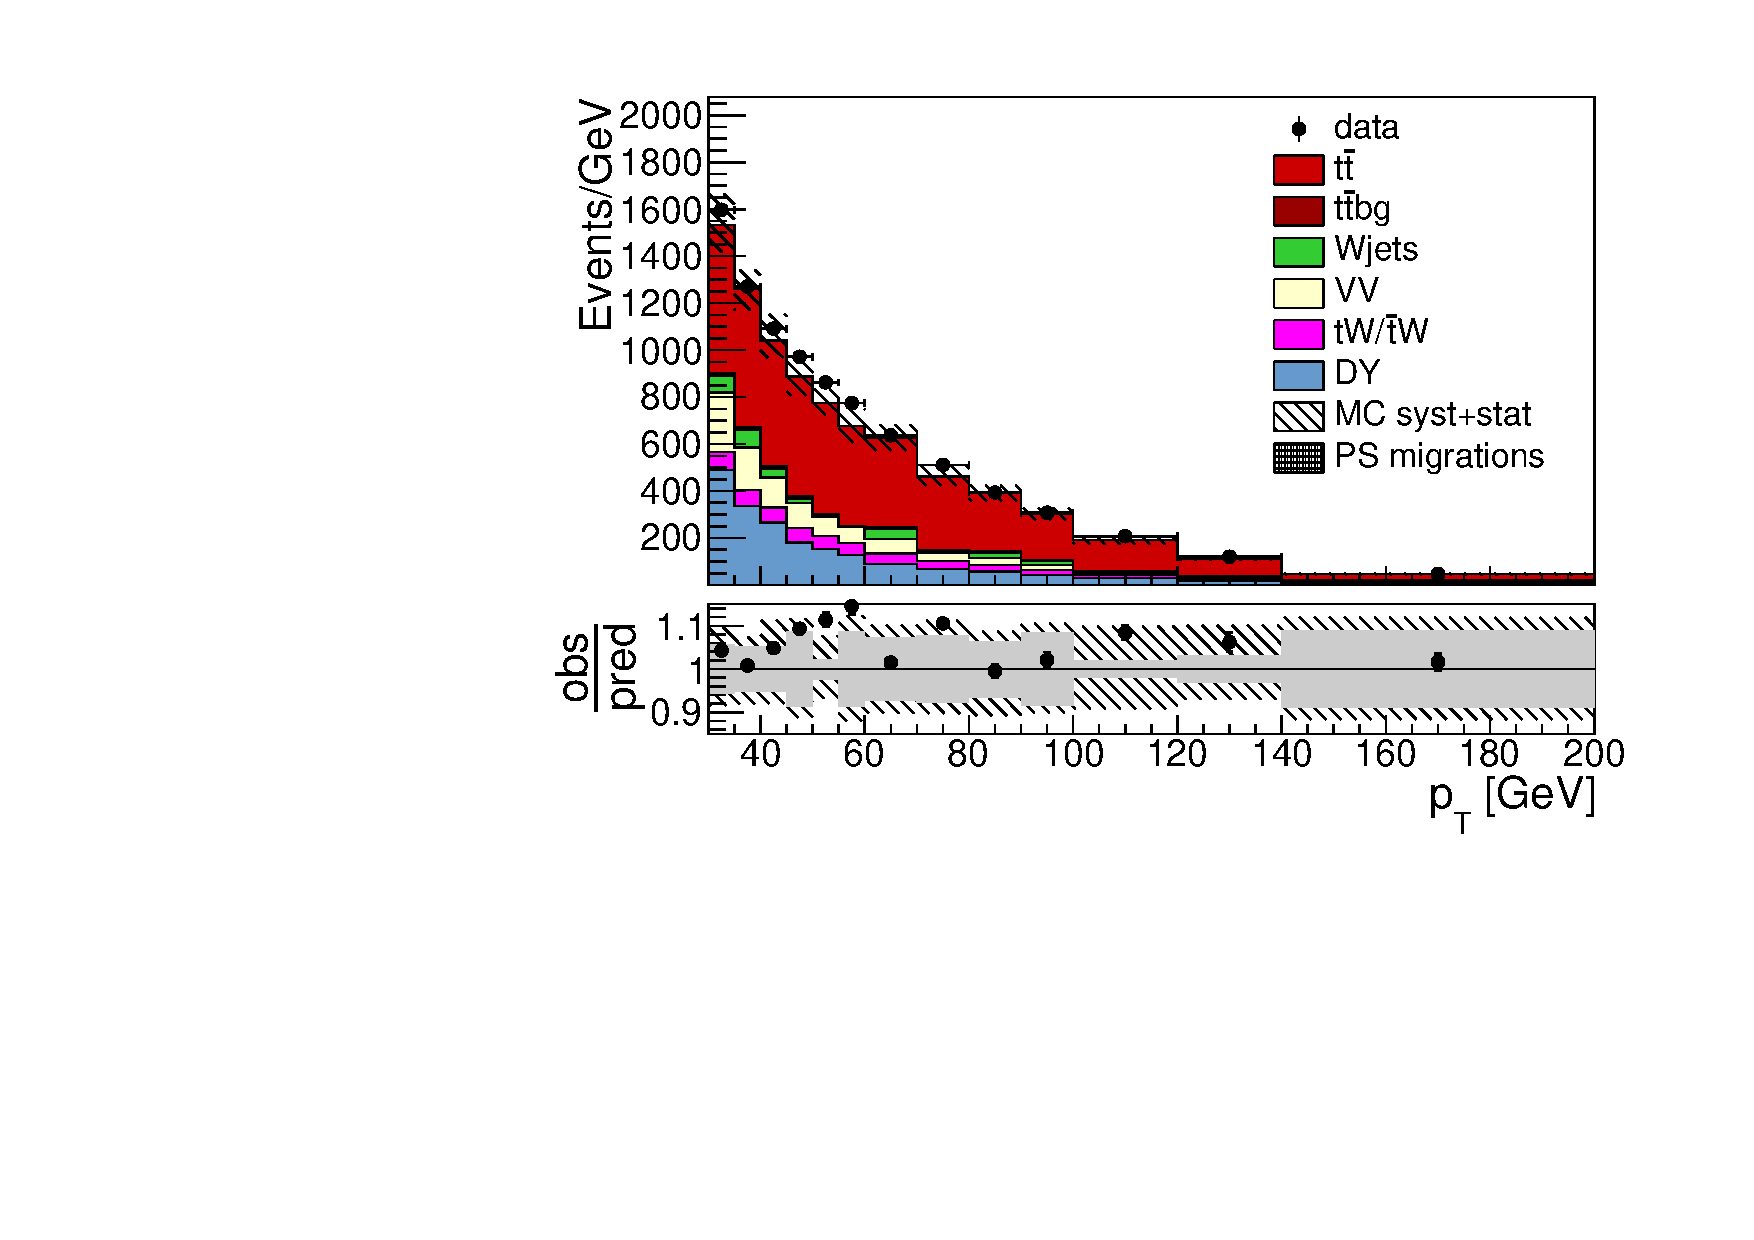
\includegraphics{CrossSection/Figures/ControlPlots/emu_sysnom/lead_jet_pt_0_1_b-jets_step_8.pdf}}
    \resizebox{0.32 \textwidth}{!}{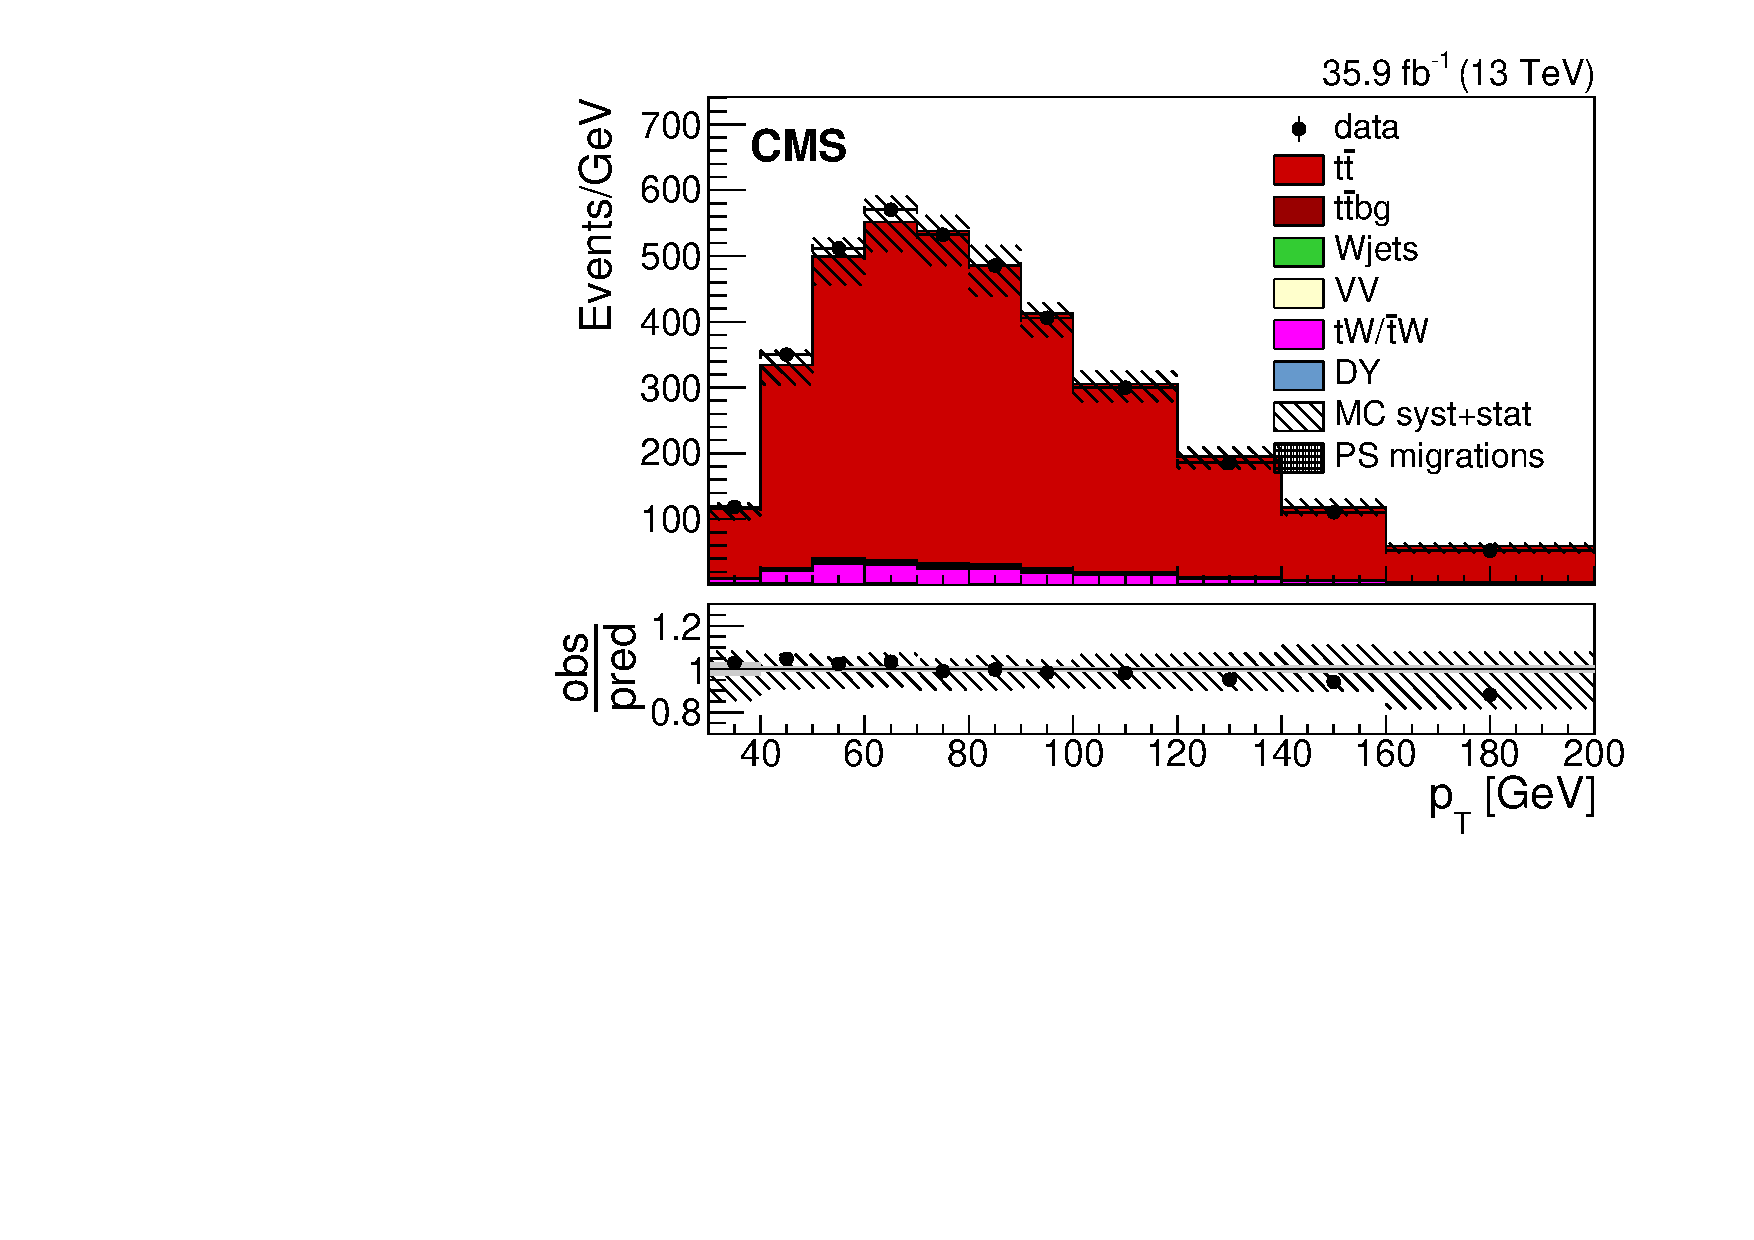
\includegraphics{CrossSection/Figures/ControlPlots/emu_sysnom/lead_jet_pt_1_1_b-jets_step_8.pdf}}
    \resizebox{0.32 \textwidth}{!}{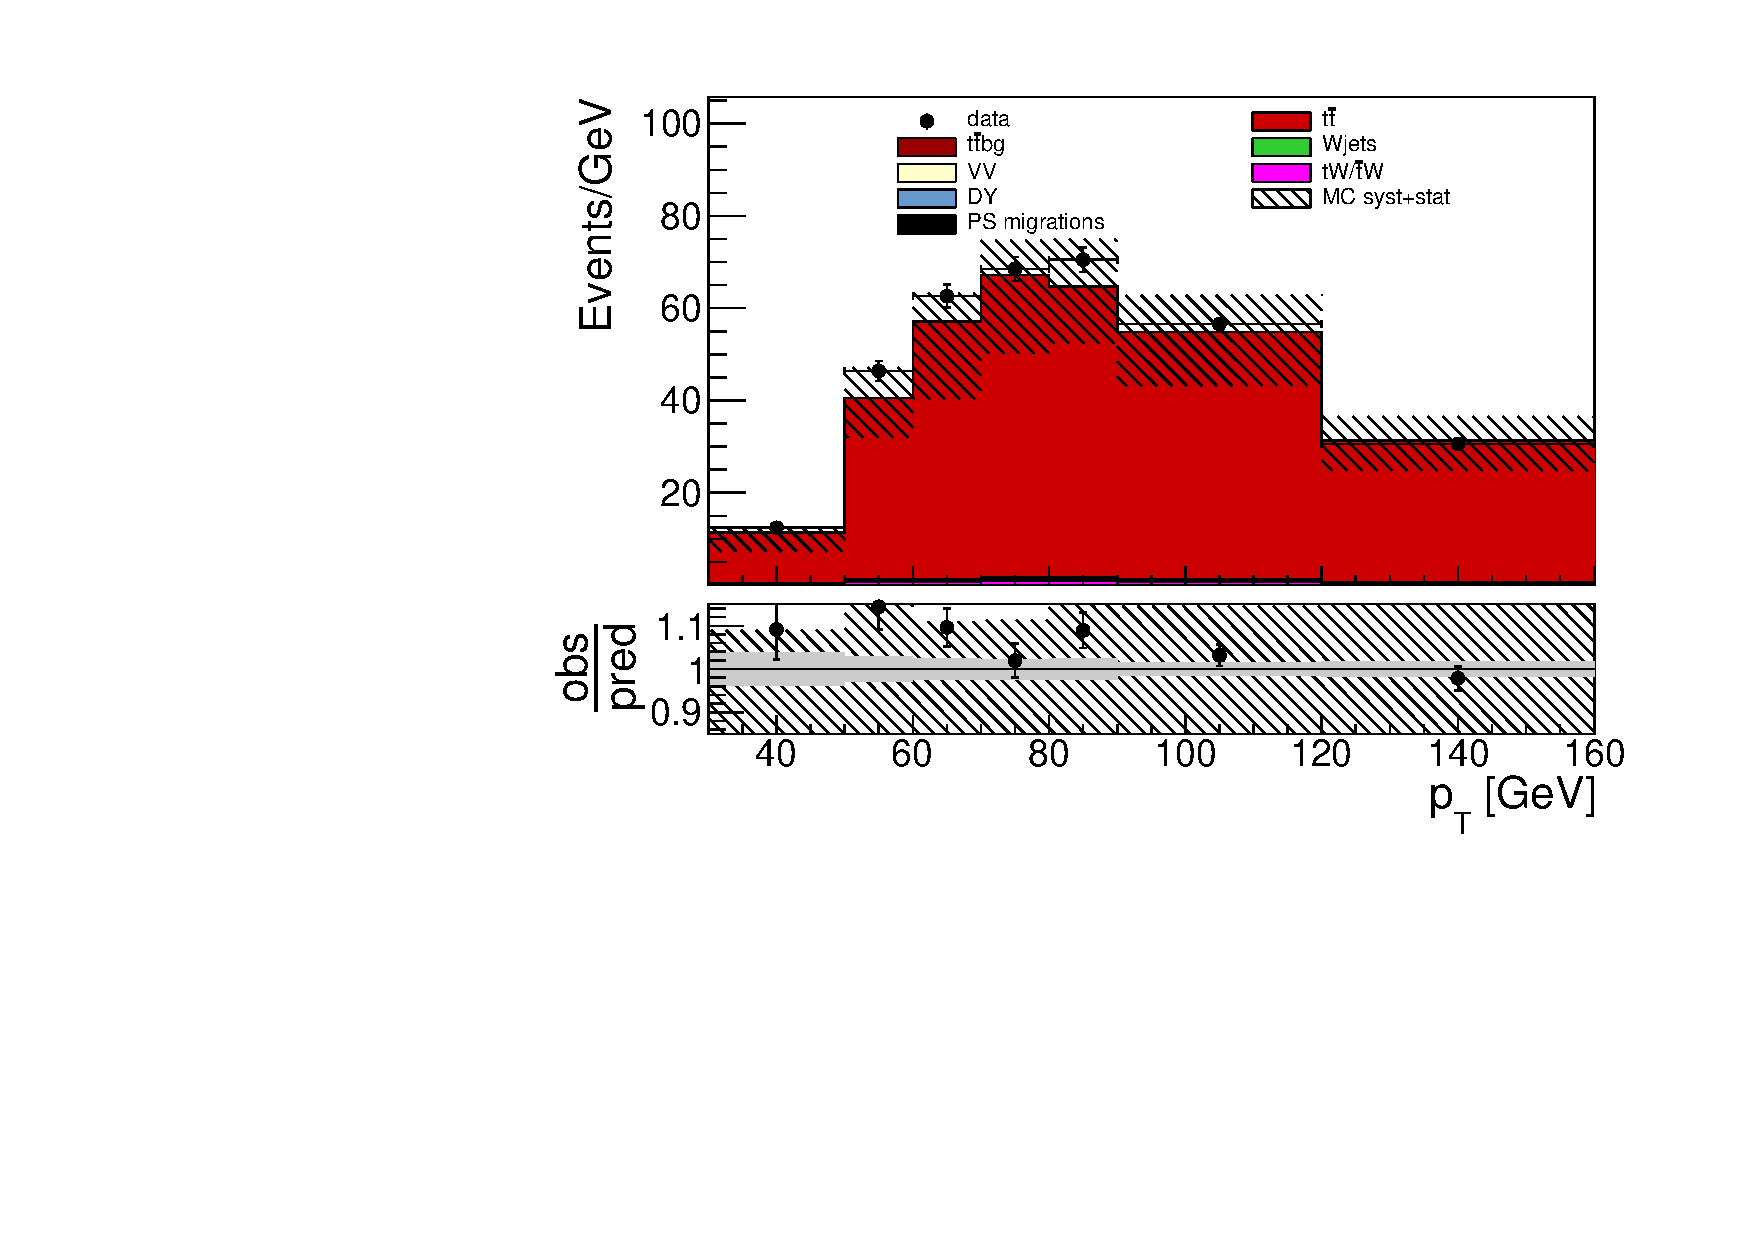
\includegraphics{CrossSection/Figures/ControlPlots/emu_sysnom/lead_jet_pt_2_1_b-jets_step_8.pdf}}
        
    \resizebox{0.32 \textwidth}{!}{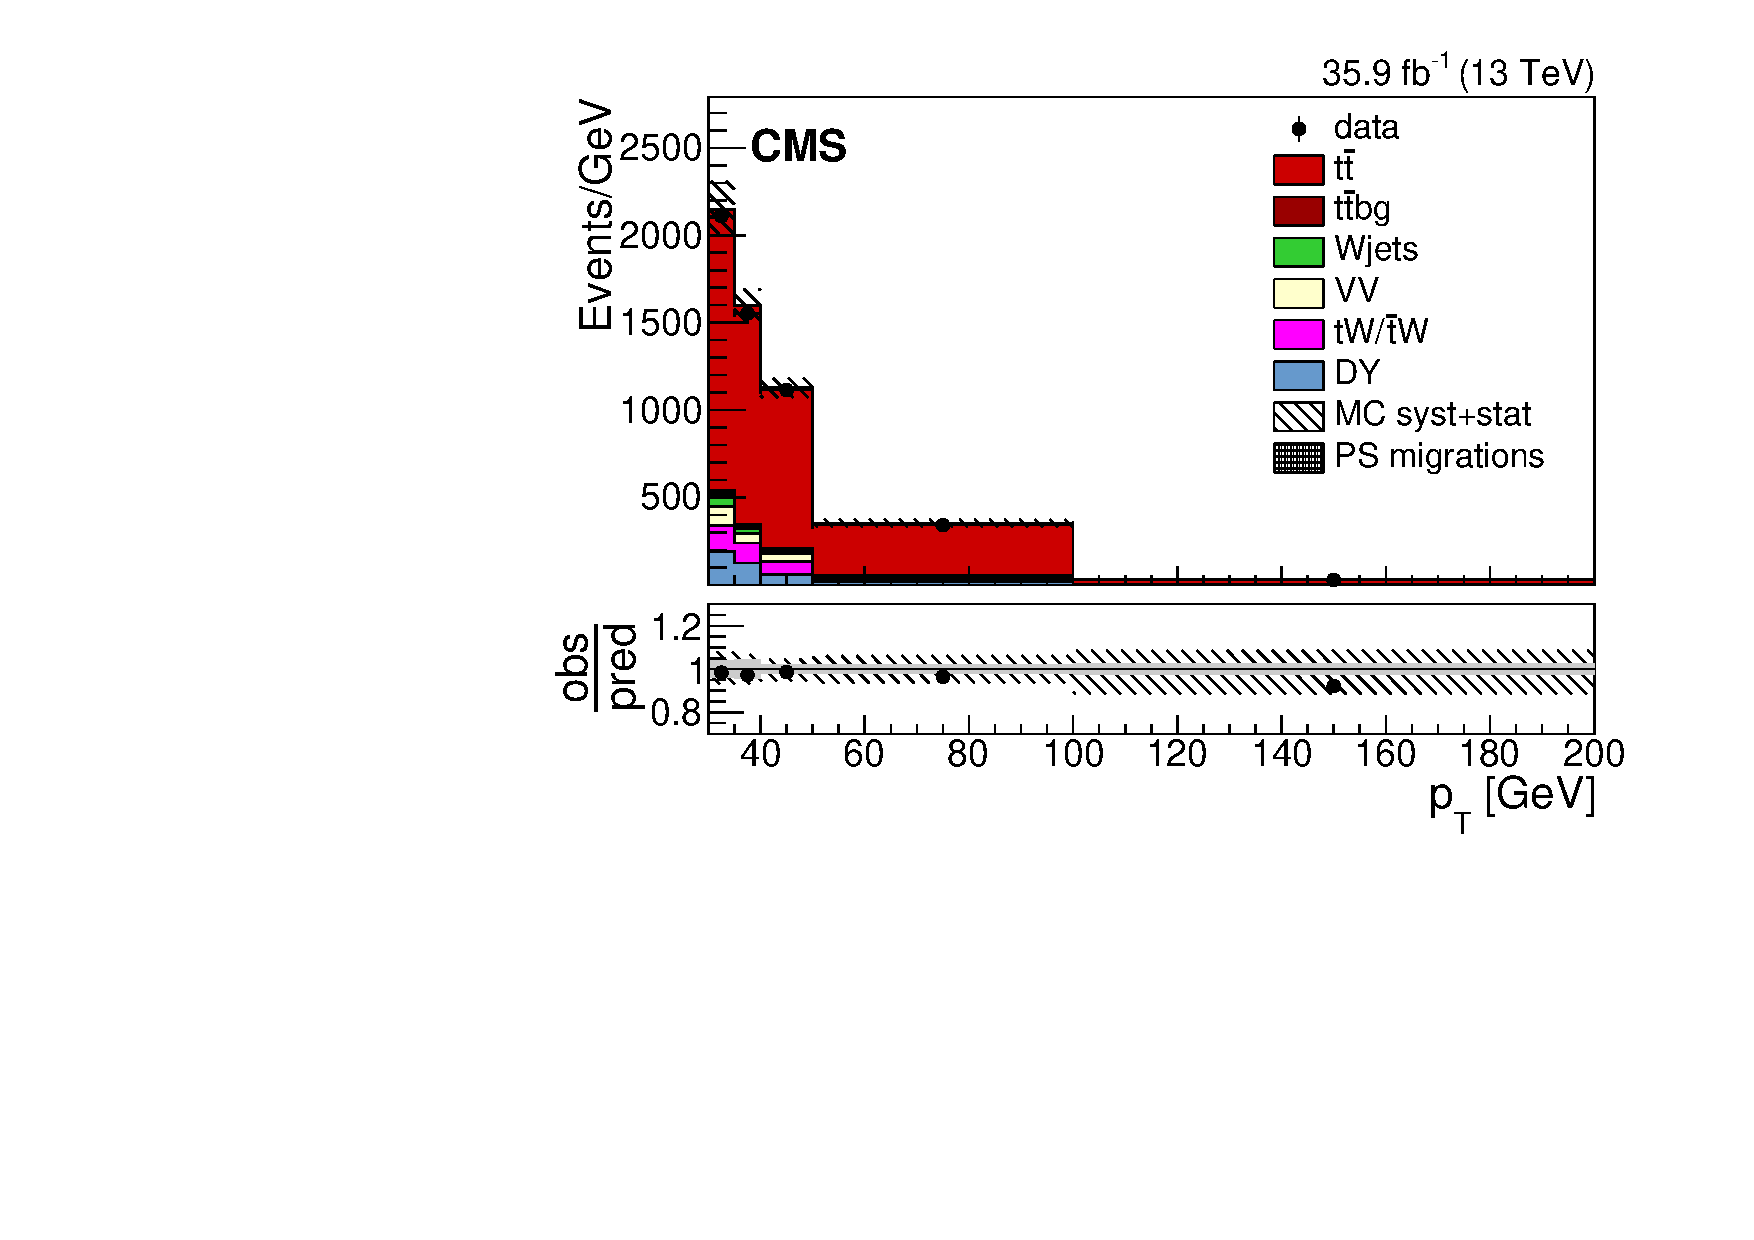
\includegraphics{CrossSection/Figures/ControlPlots/emu_sysnom/second_jet_pt_0_2_b-jets_step_8.pdf}}
    \resizebox{0.32 \textwidth}{!}{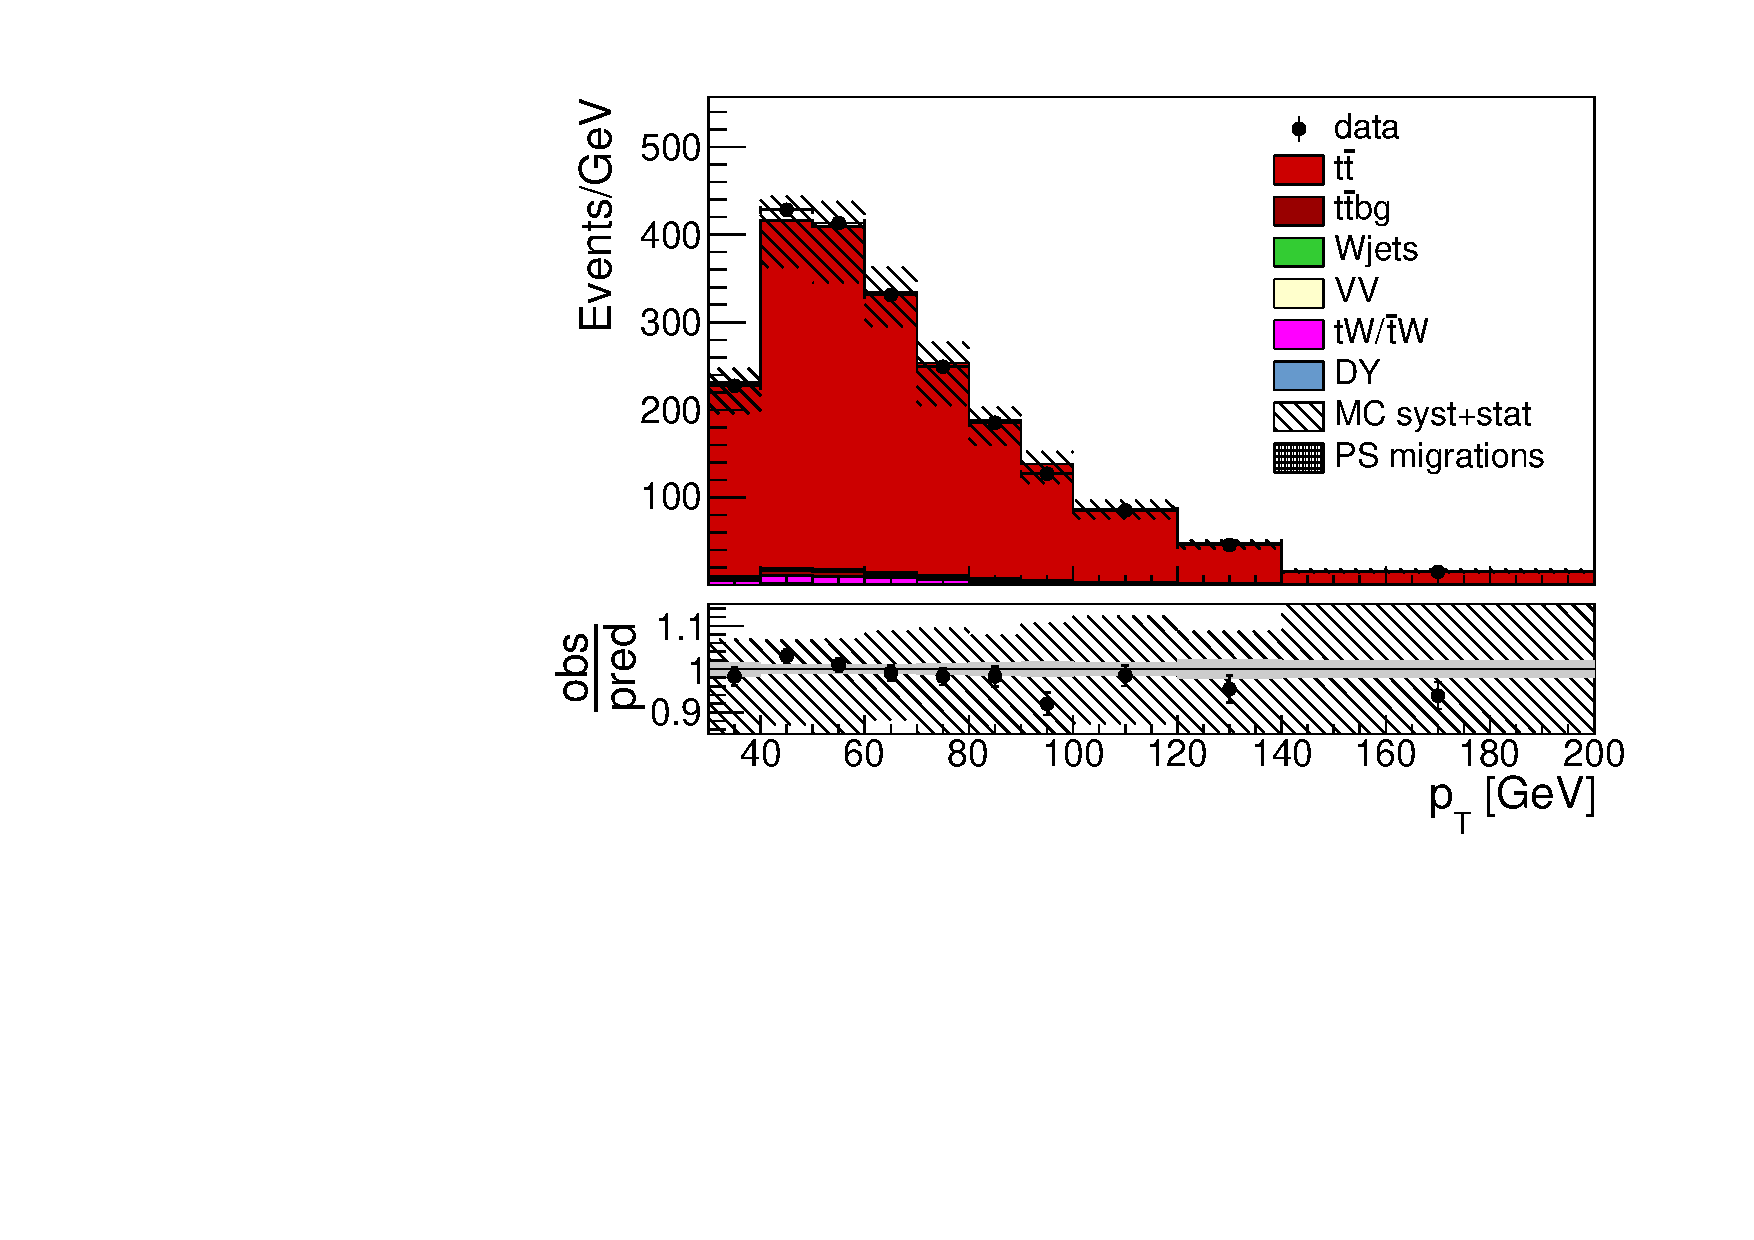
\includegraphics{CrossSection/Figures/ControlPlots/emu_sysnom/second_jet_pt_1_2_b-jets_step_8.pdf}}
    \resizebox{0.32 \textwidth}{!}{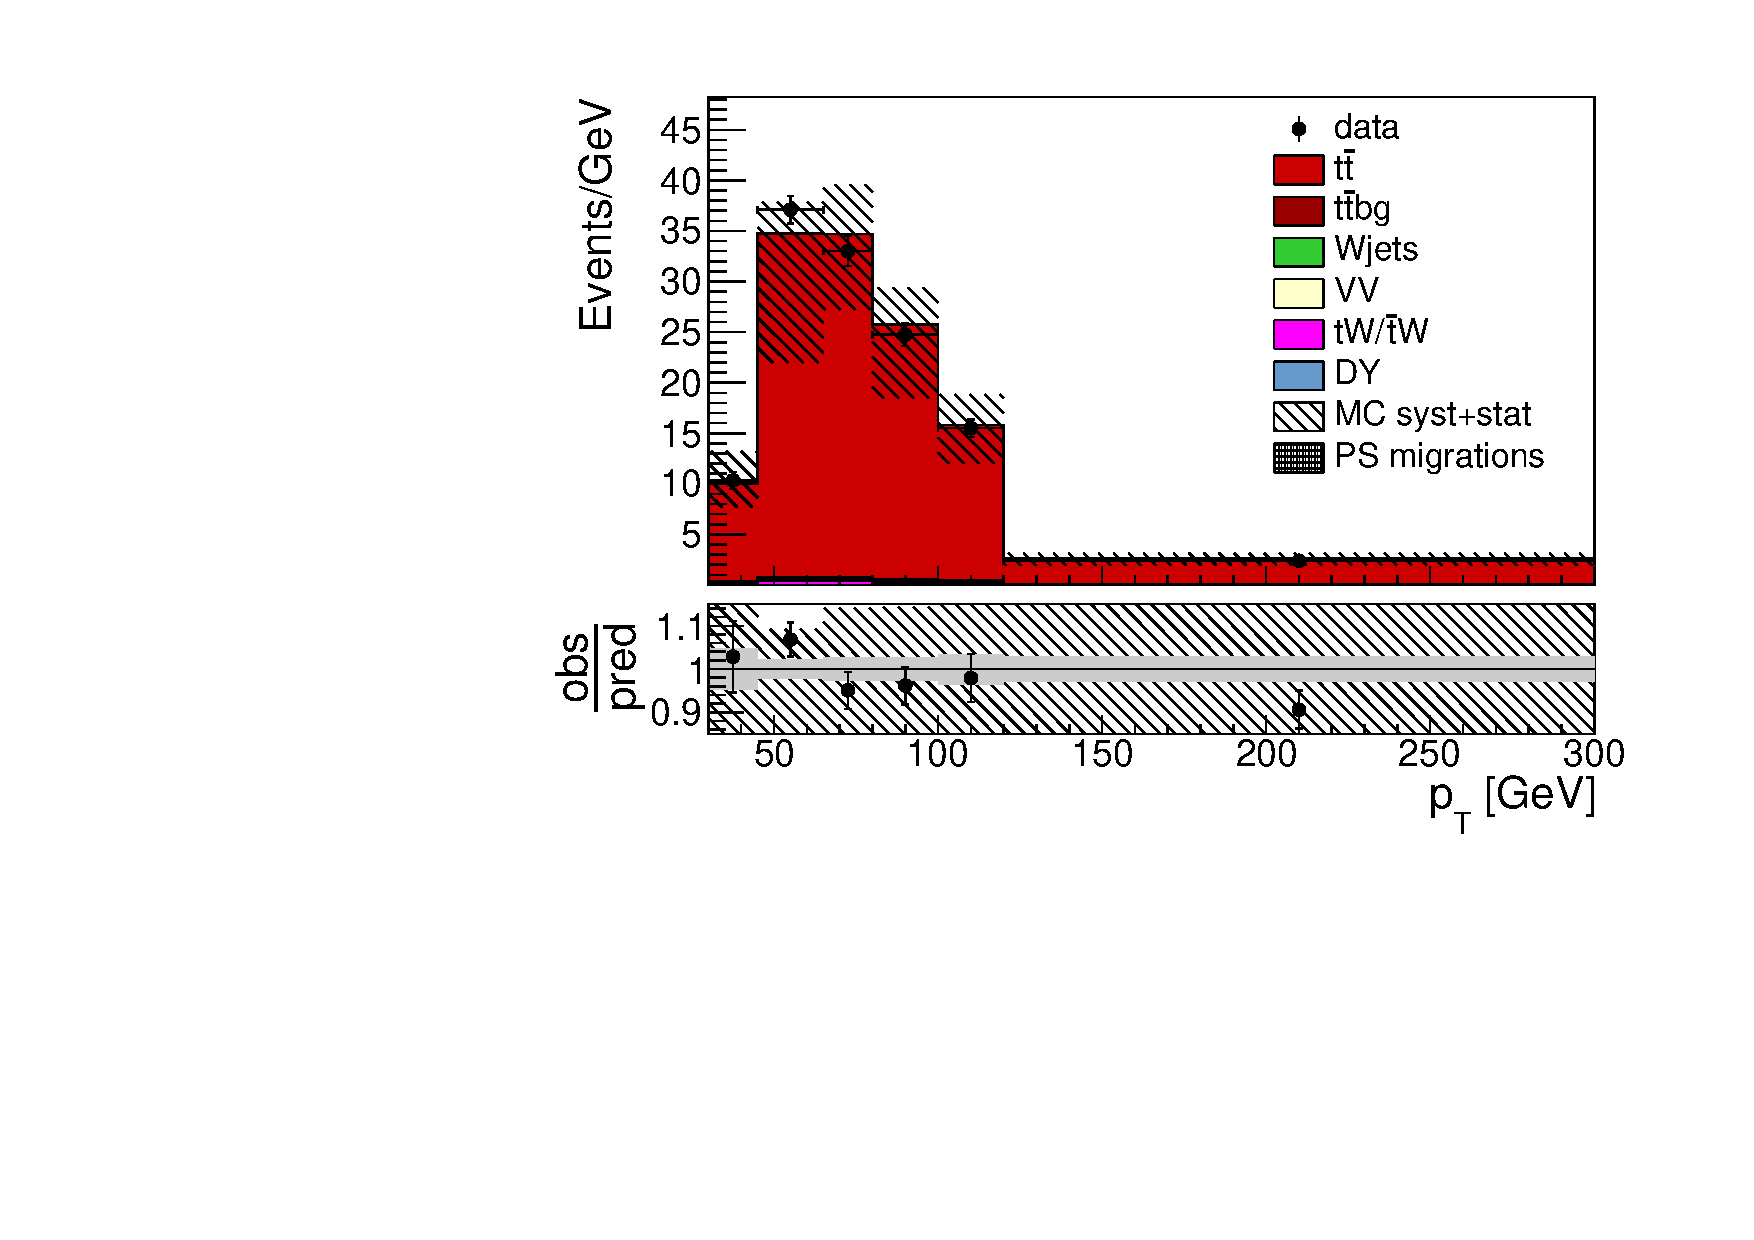
\includegraphics{CrossSection/Figures/ControlPlots/emu_sysnom/second_jet_pt_2_2_b-jets_step_8.pdf}}

    \resizebox{0.32 \textwidth}{!}{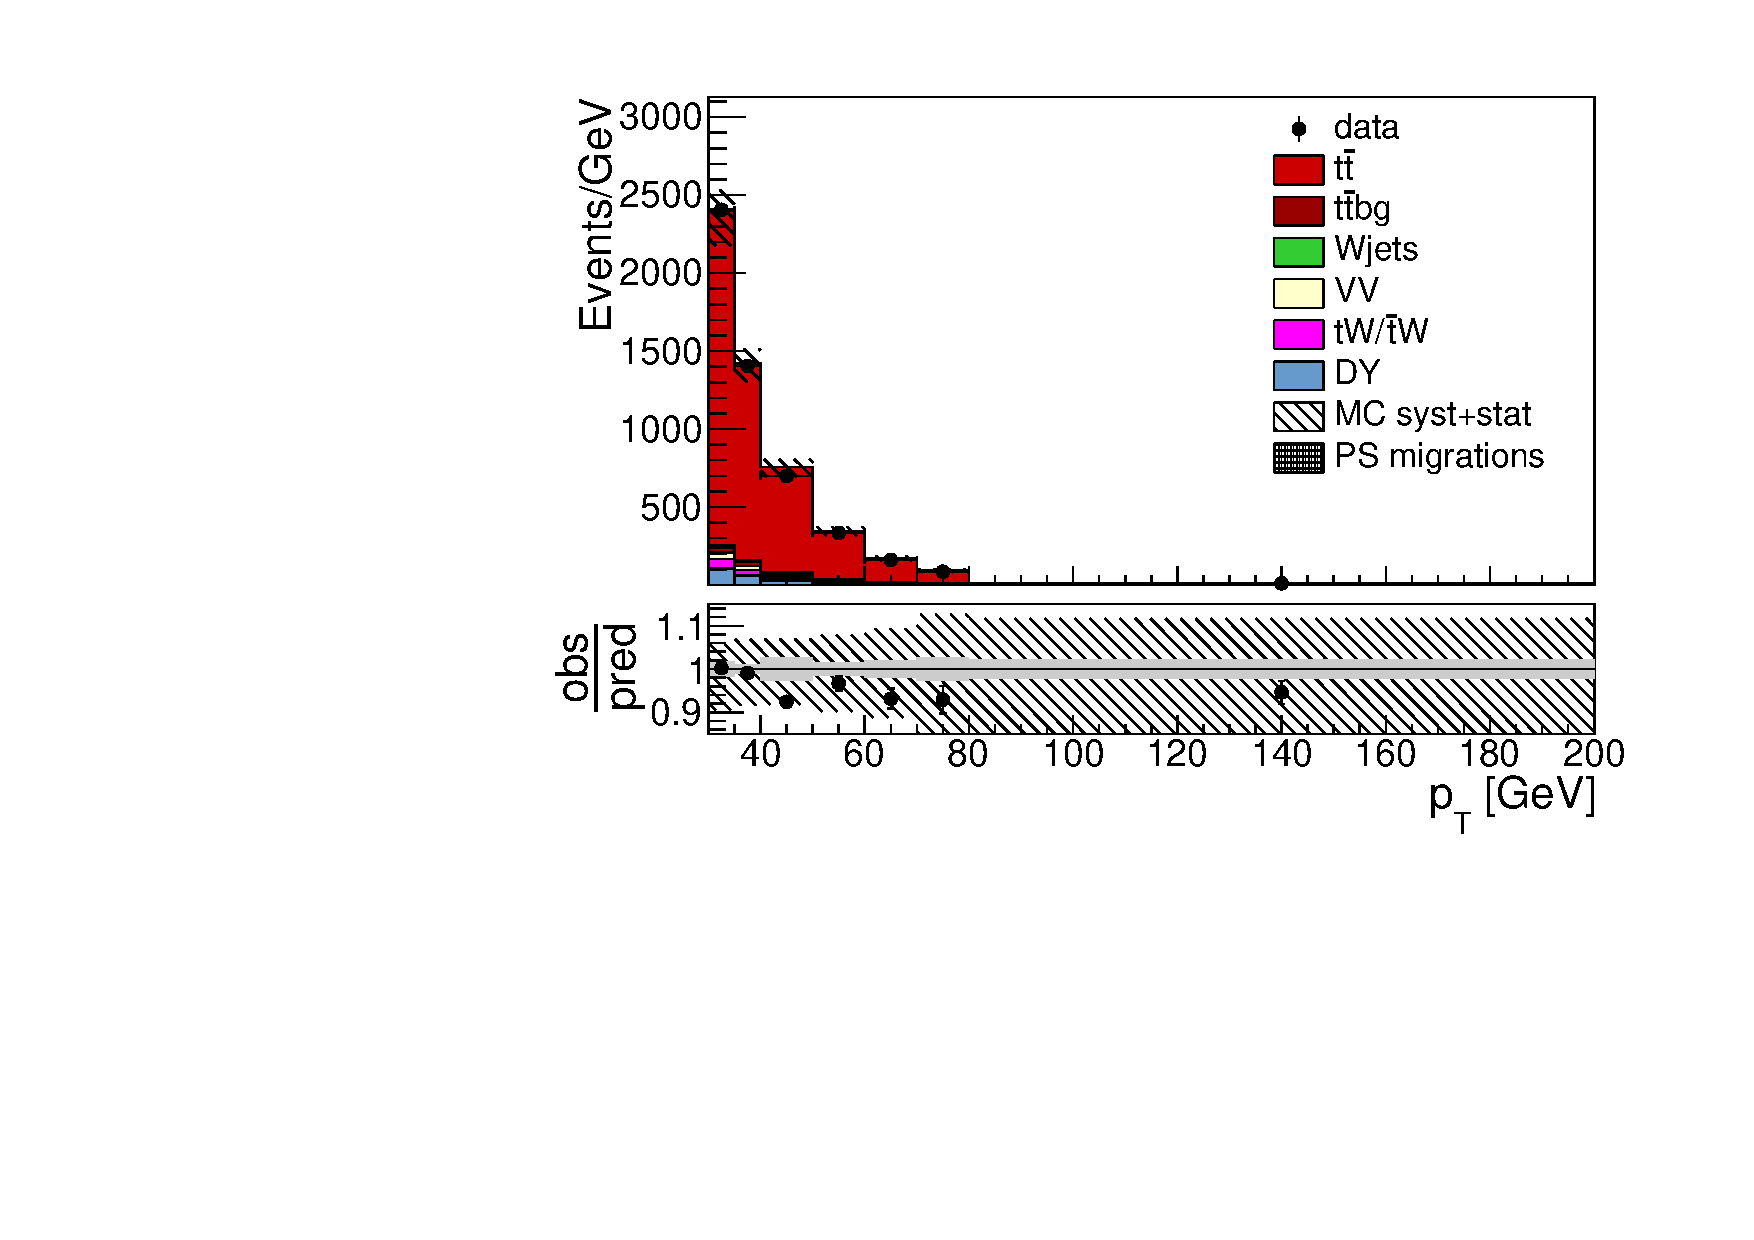
\includegraphics{CrossSection/Figures/ControlPlots/emu_sysnom/third_jet_pt_0_3_b-jets_step_8.pdf}}
    \resizebox{0.32 \textwidth}{!}{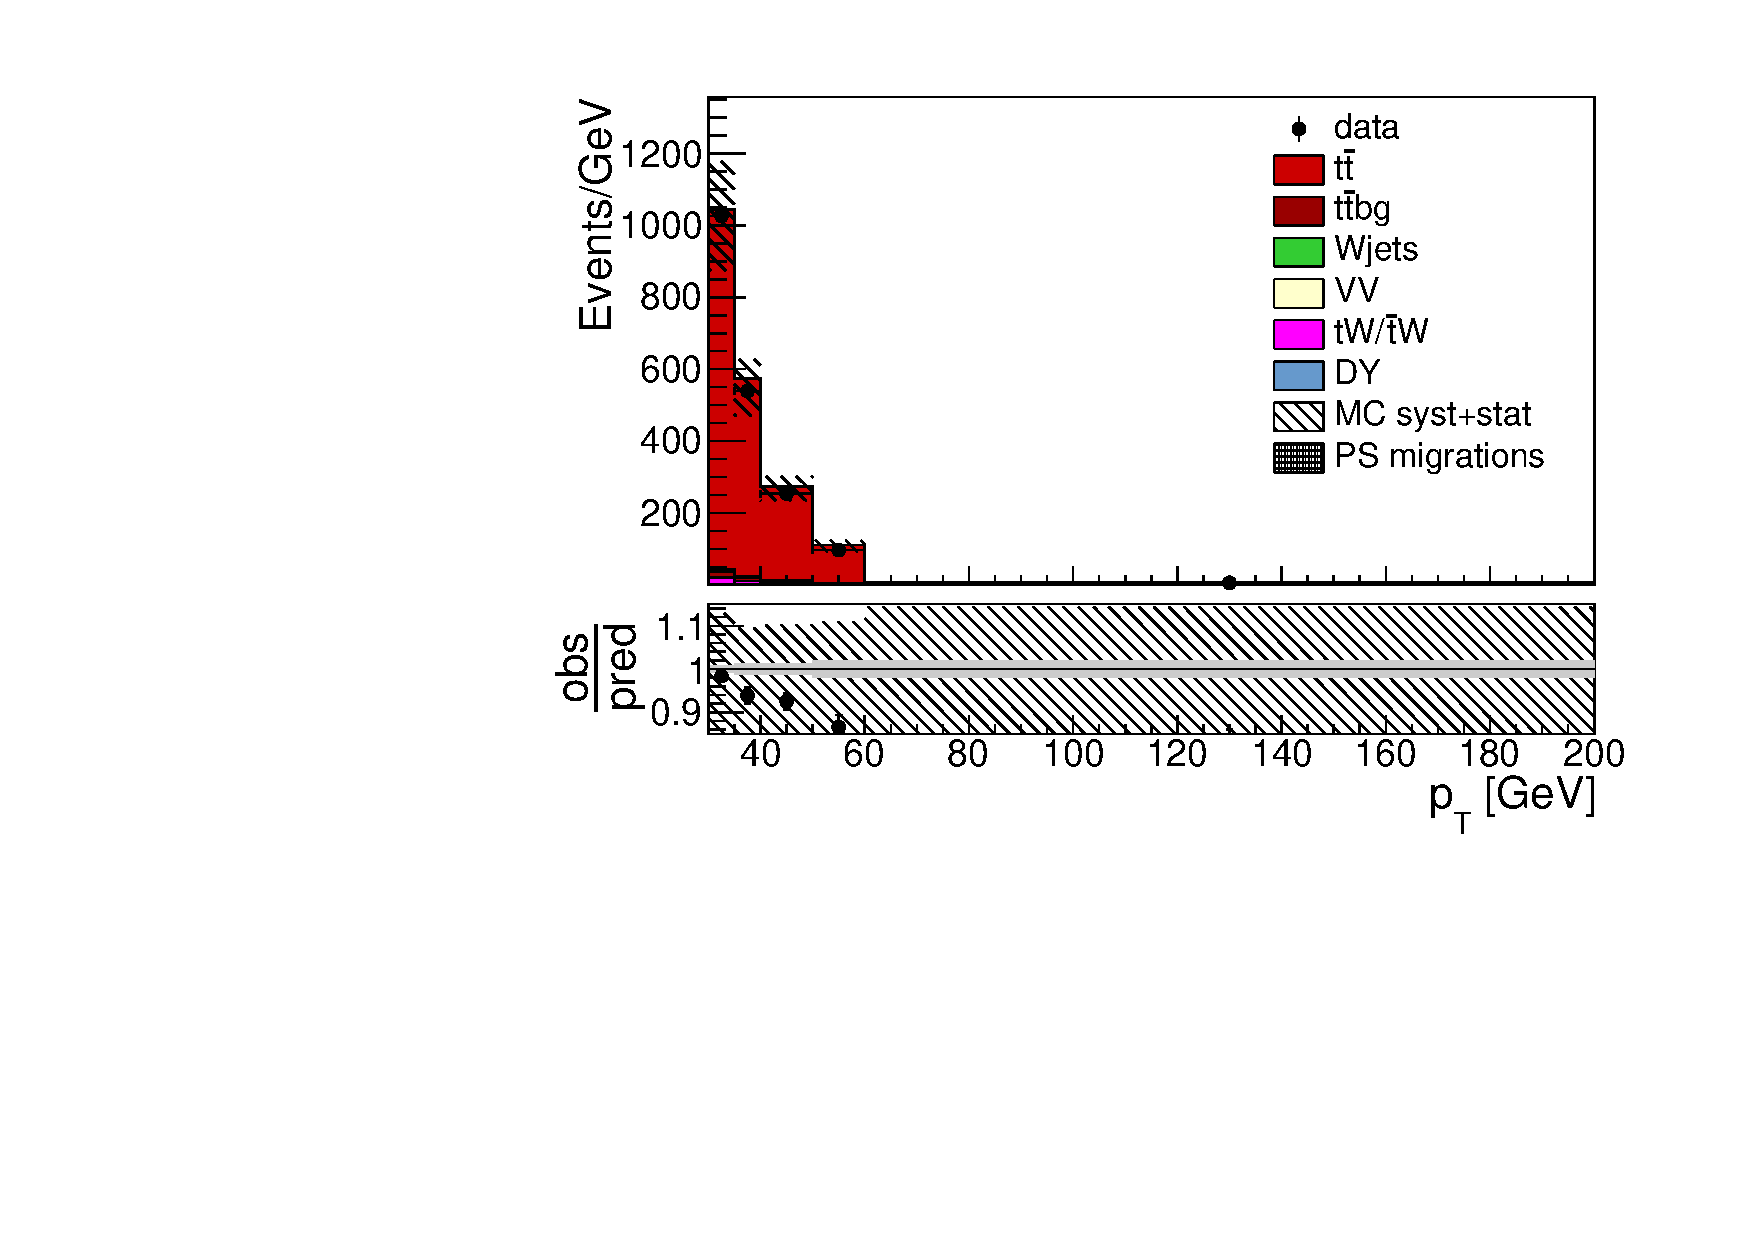
\includegraphics{CrossSection/Figures/ControlPlots/emu_sysnom/third_jet_pt_1_3_b-jets_step_8.pdf}}
    \resizebox{0.32 \textwidth}{!}{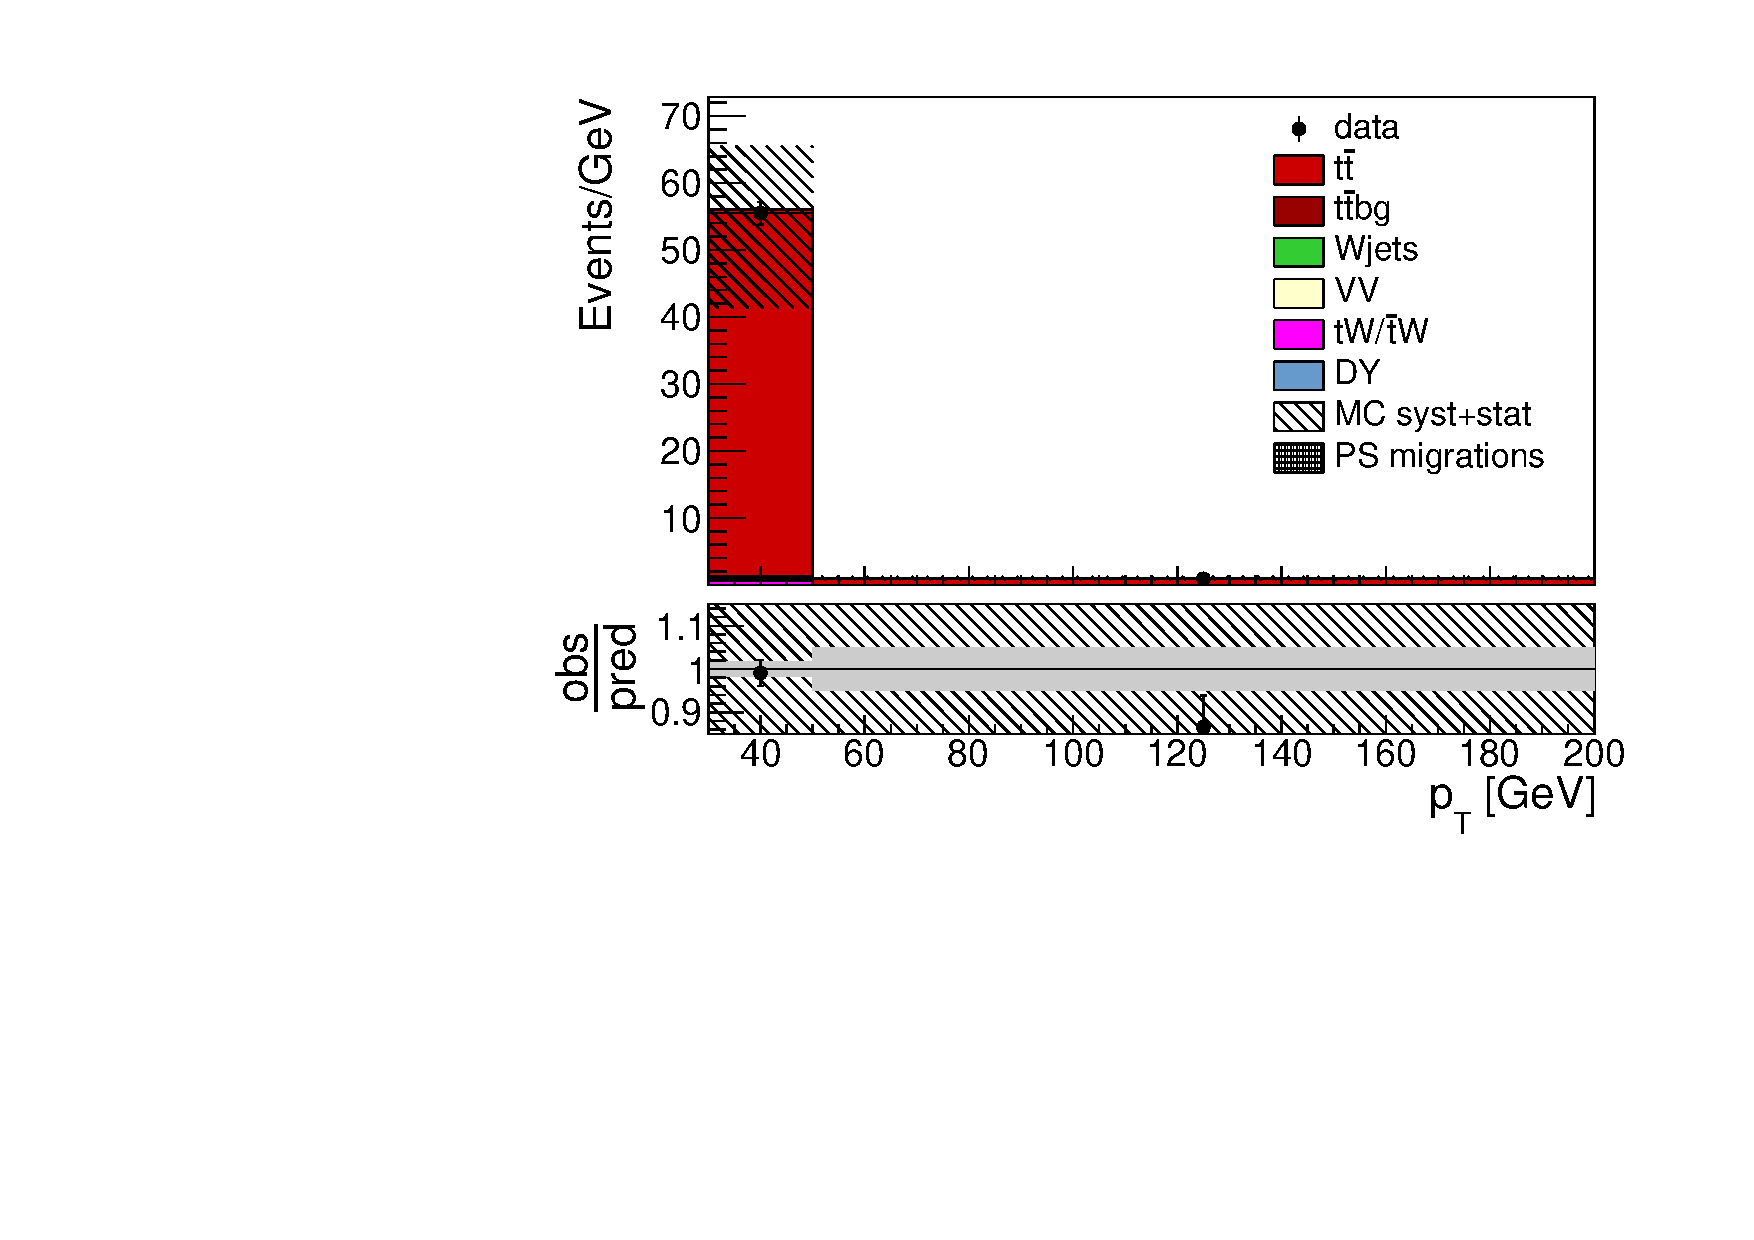
\includegraphics{CrossSection/Figures/ControlPlots/emu_sysnom/third_jet_pt_2_3_b-jets_step_8.pdf}}  

\caption{Template distributions for events in the \emu channel with zero as well as three or
  more b-tagged jets (left column), One b-tagged jet (middle column) or three b-tagged jets (right column). The distributions show the total event yield for zero (top) and the trailing jet pt for one (second from top),
  two (second from bottom) or three or more (bottom) additional jets. 
  The hatched bands correspond to the total uncertainty on the predicted number of events. The ratios of the event yields in data and the sum of the
  predicted yields are shown at the bottom of each plot. Here, the solid
  gray band represents the contribution of the statistical uncertainty.  
       \label{fig:xsec_emu_inputdistr}}
  \end{center}
\end{figure}

\begin{figure}[htbp!]
  \begin{center}
    \resizebox{0.40 \textwidth}{!}{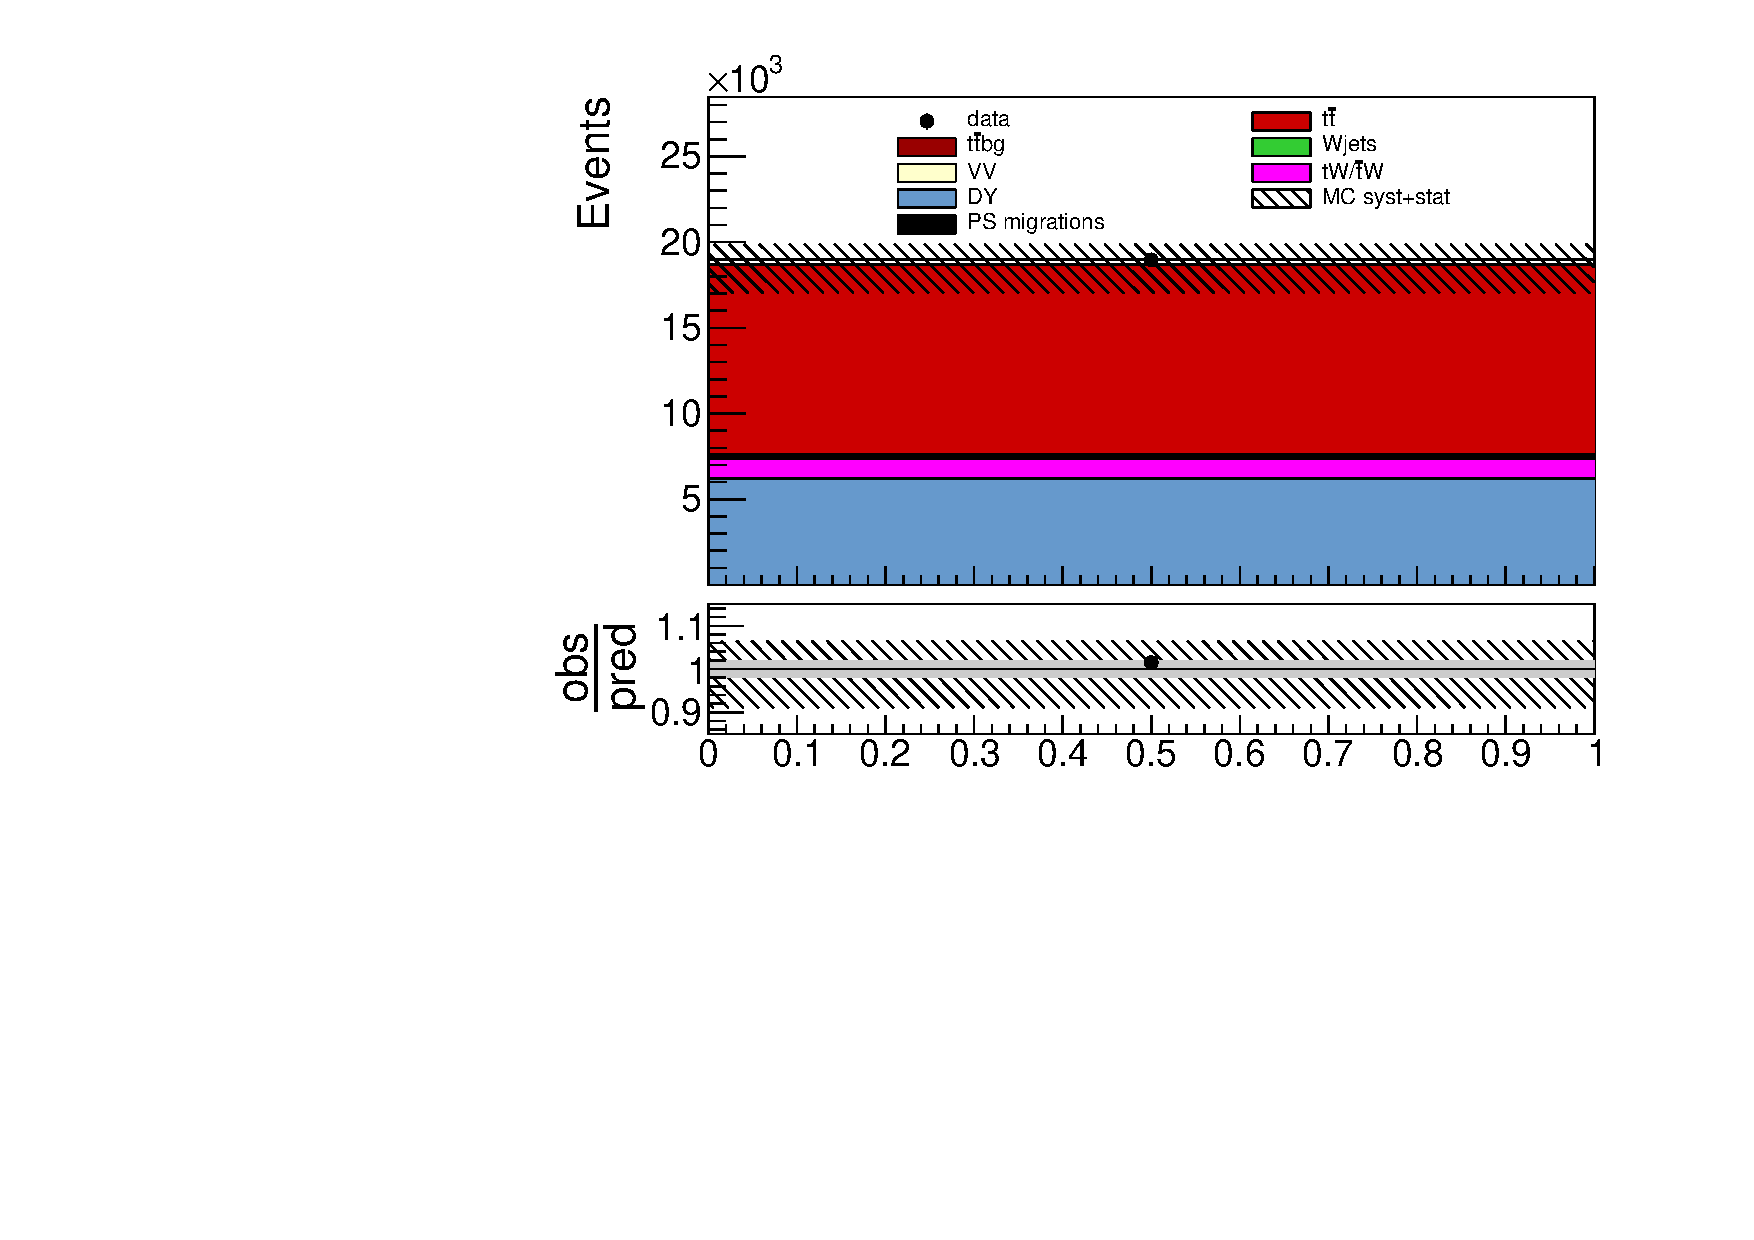
\includegraphics{CrossSection/Figures/ControlPlots/mumu_sysnom/total_1_0_b-jets_step_8.pdf}}
    \resizebox{0.40 \textwidth}{!}{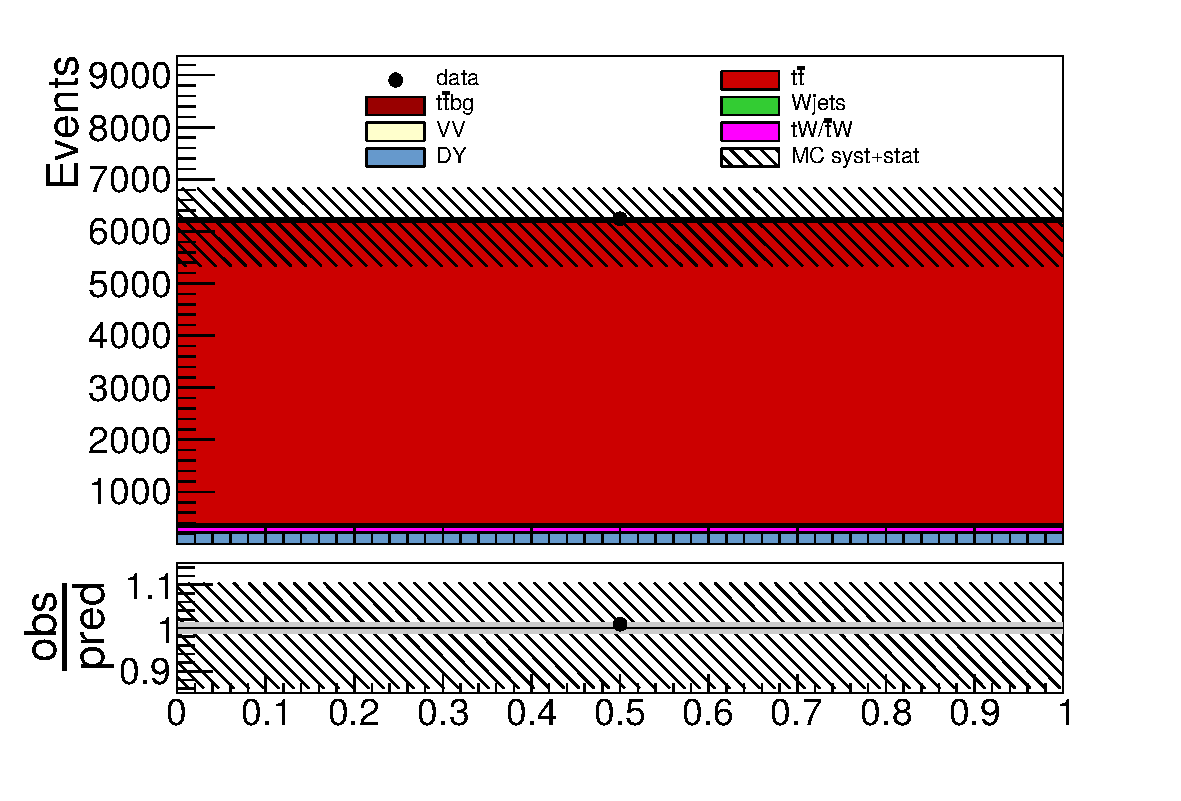
\includegraphics{CrossSection/Figures/ControlPlots/mumu_sysnom/total_2_0_b-jets_step_8.pdf}} \\

    \resizebox{0.40 \textwidth}{!}{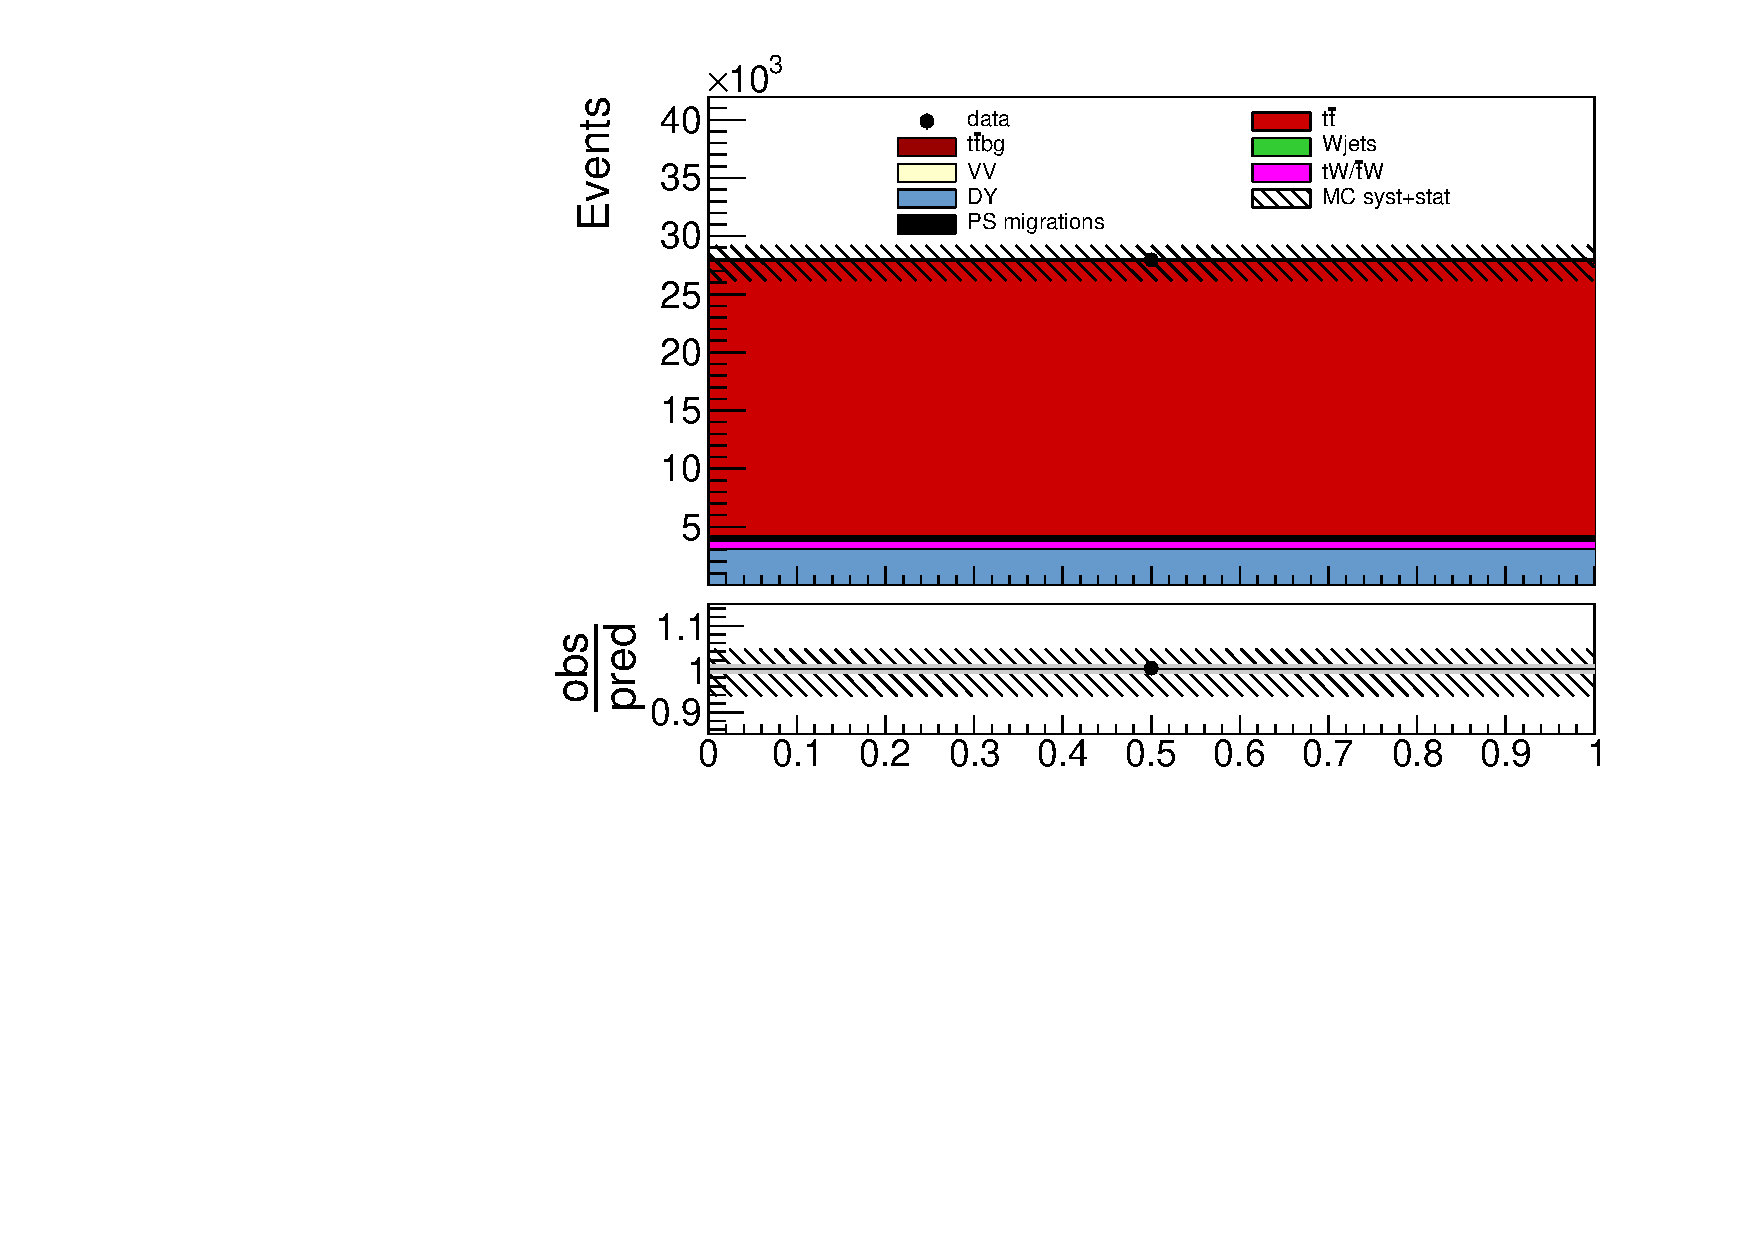
\includegraphics{CrossSection/Figures/ControlPlots/mumu_sysnom/total_1_1_b-jets_step_8.pdf}}
    \resizebox{0.40 \textwidth}{!}{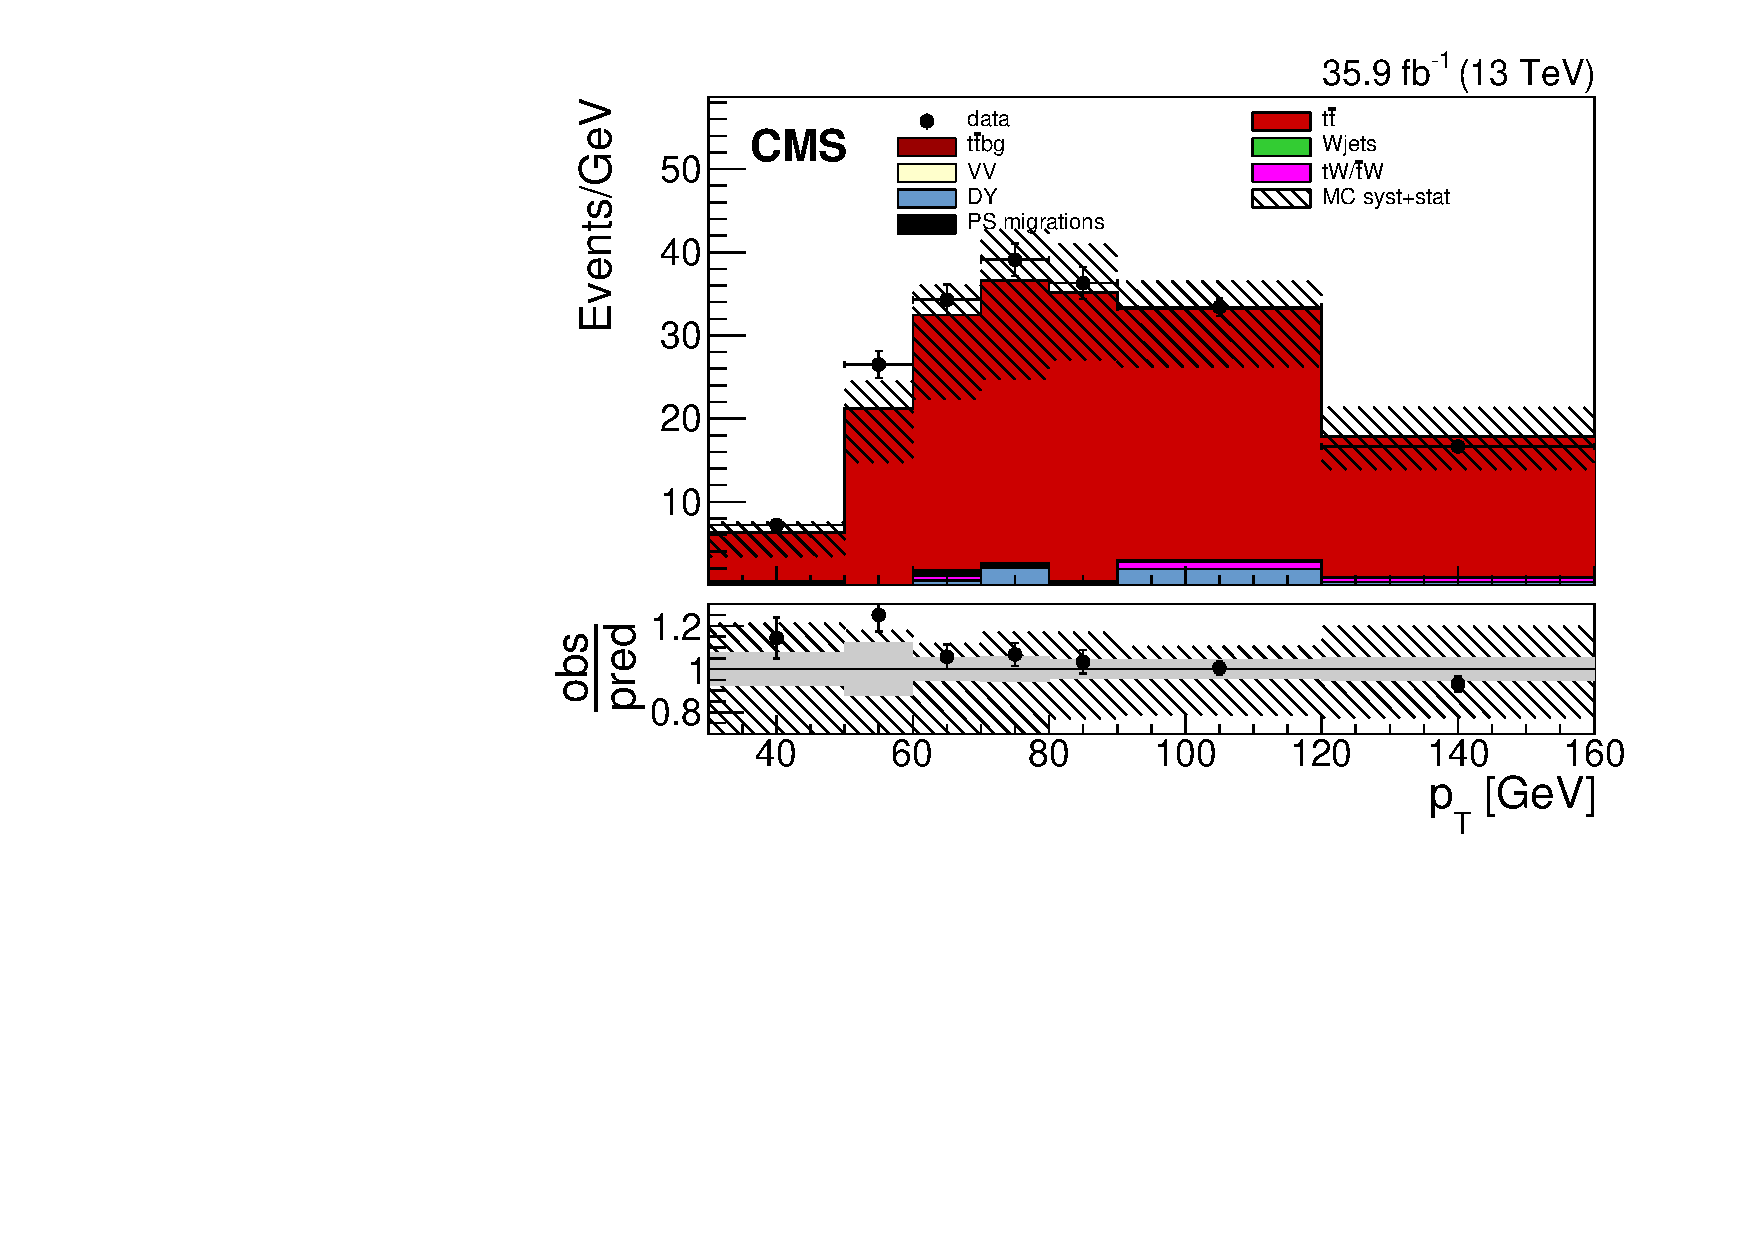
\includegraphics{CrossSection/Figures/ControlPlots/mumu_sysnom/lead_jet_pt_2_1_b-jets_step_8.pdf}}\\
        
    \resizebox{0.4 \textwidth}{!}{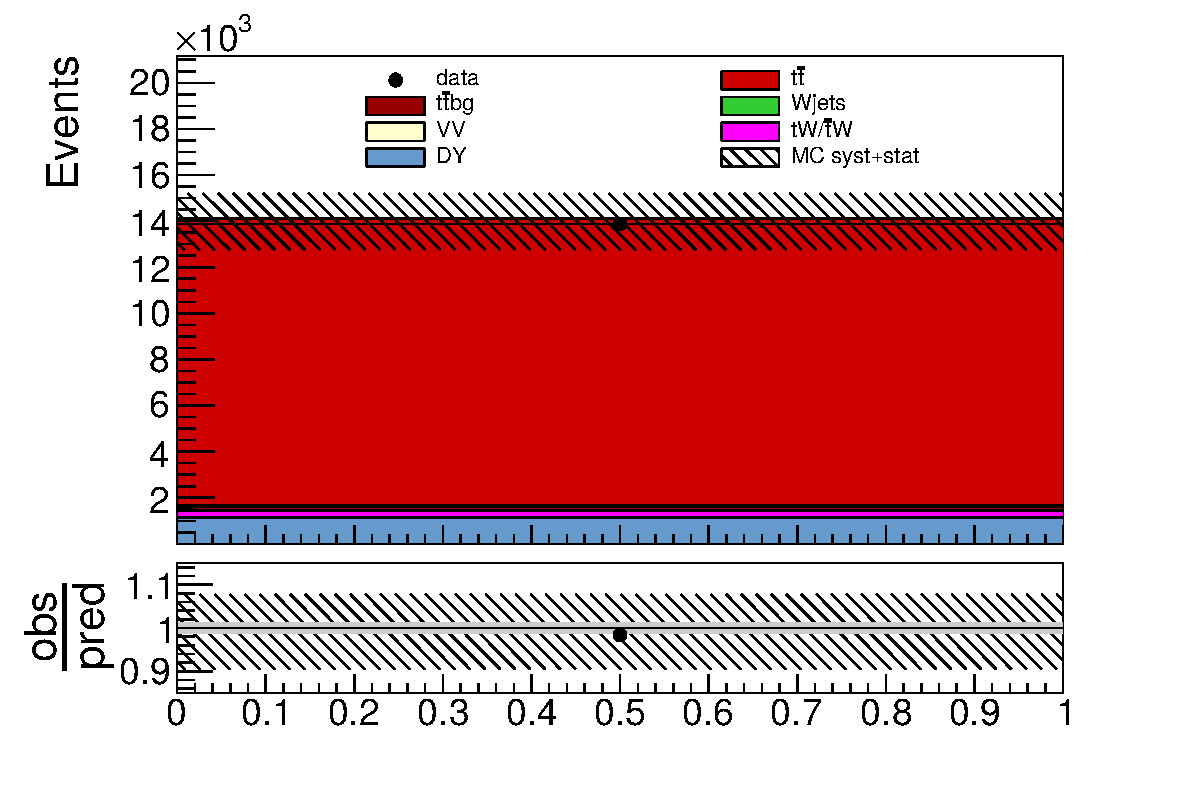
\includegraphics{CrossSection/Figures/ControlPlots/mumu_sysnom/total_1_2_b-jets_step_8.pdf}}
    \resizebox{0.4 \textwidth}{!}{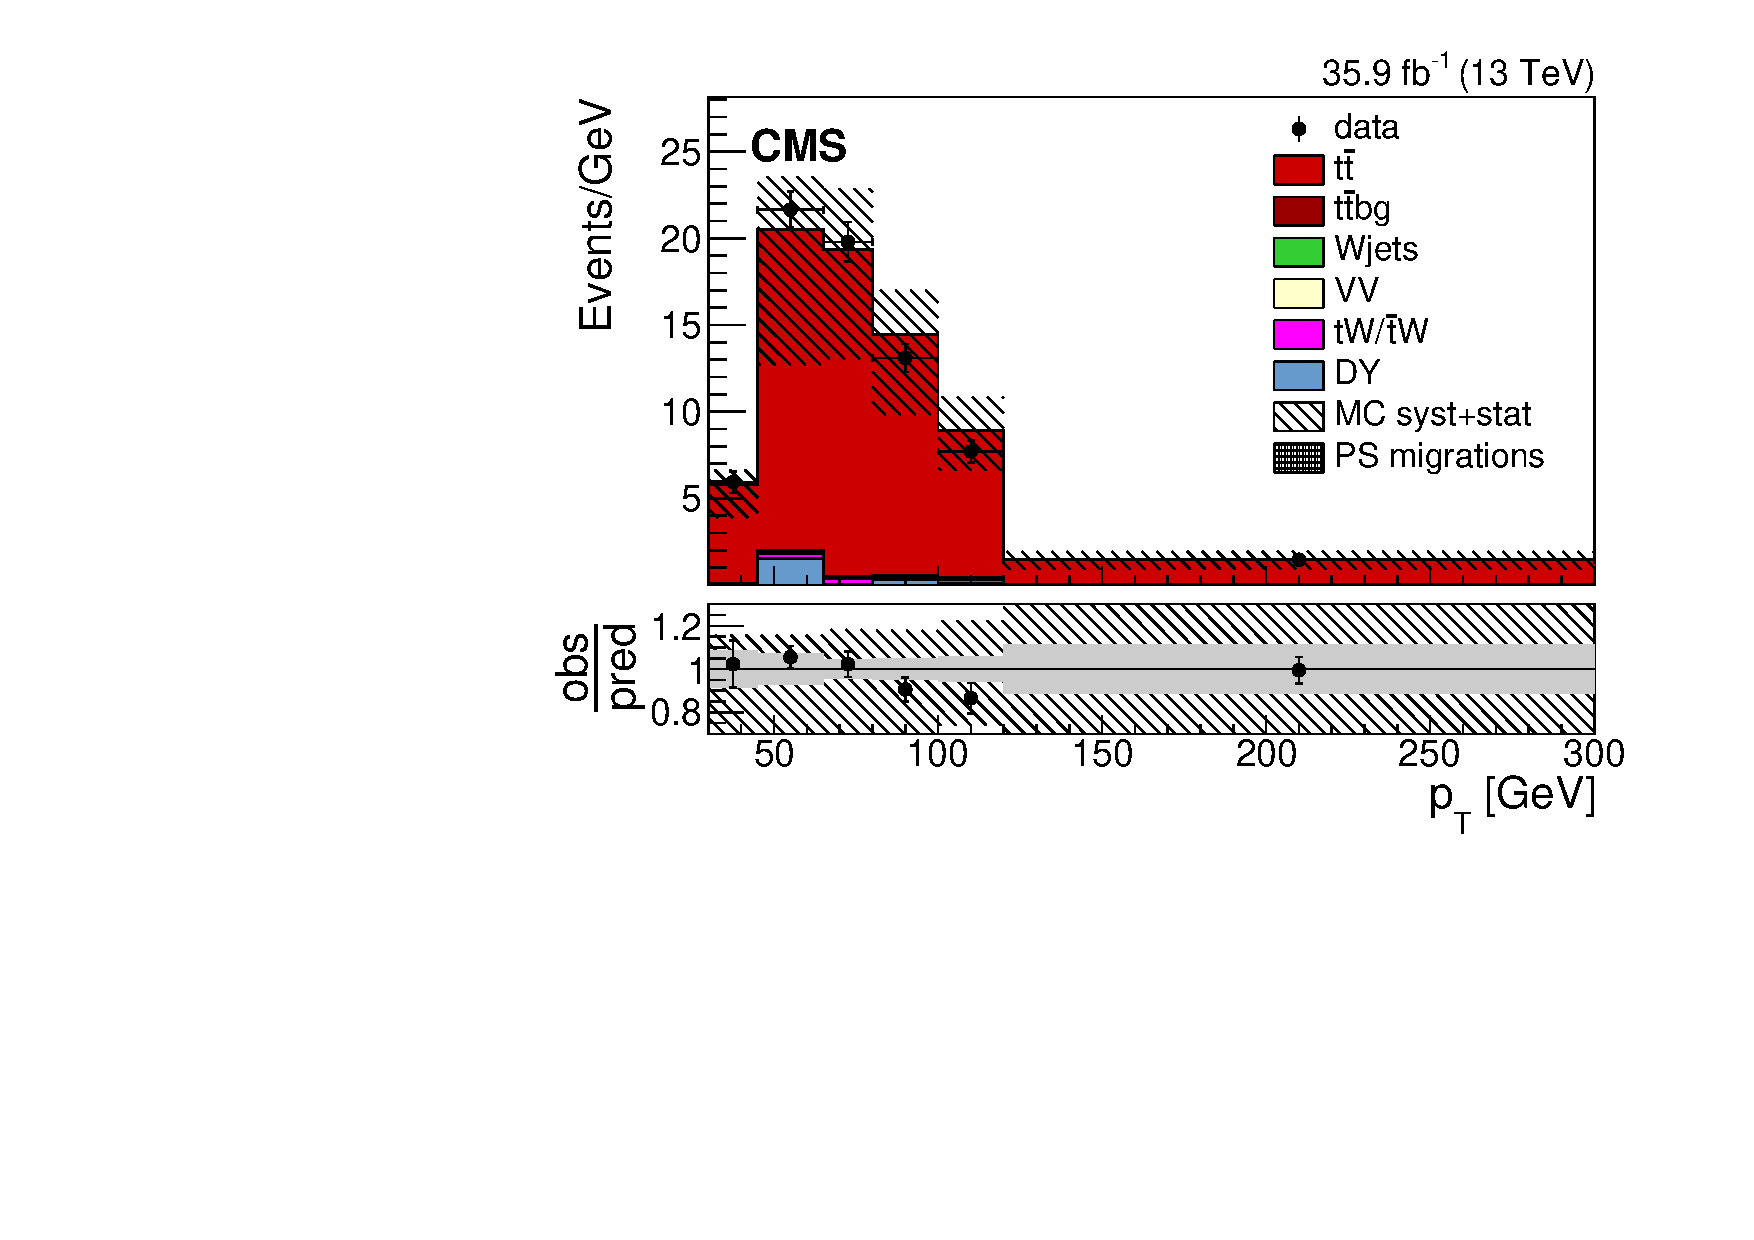
\includegraphics{CrossSection/Figures/ControlPlots/mumu_sysnom/second_jet_pt_2_2_b-jets_step_8.pdf}}\\

    \resizebox{0.4 \textwidth}{!}{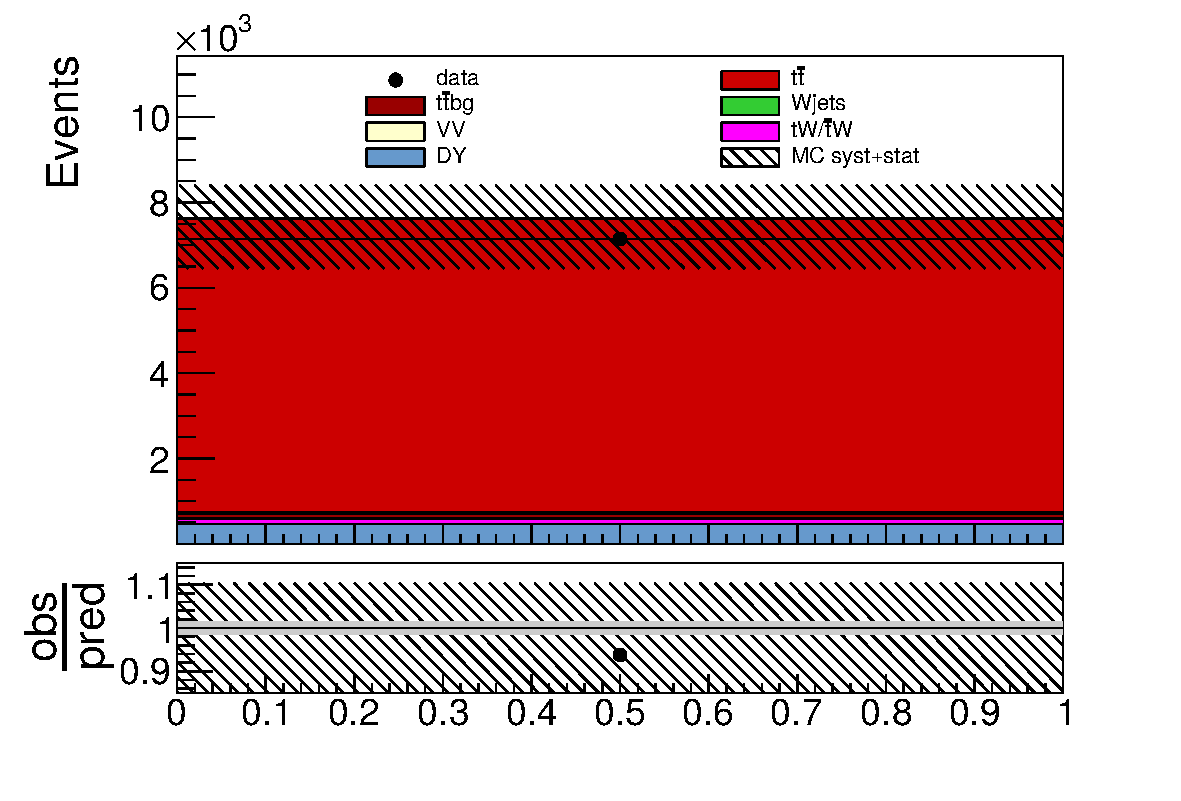
\includegraphics{CrossSection/Figures/ControlPlots/mumu_sysnom/total_1_3_b-jets_step_8.pdf}}
    \resizebox{0.4 \textwidth}{!}{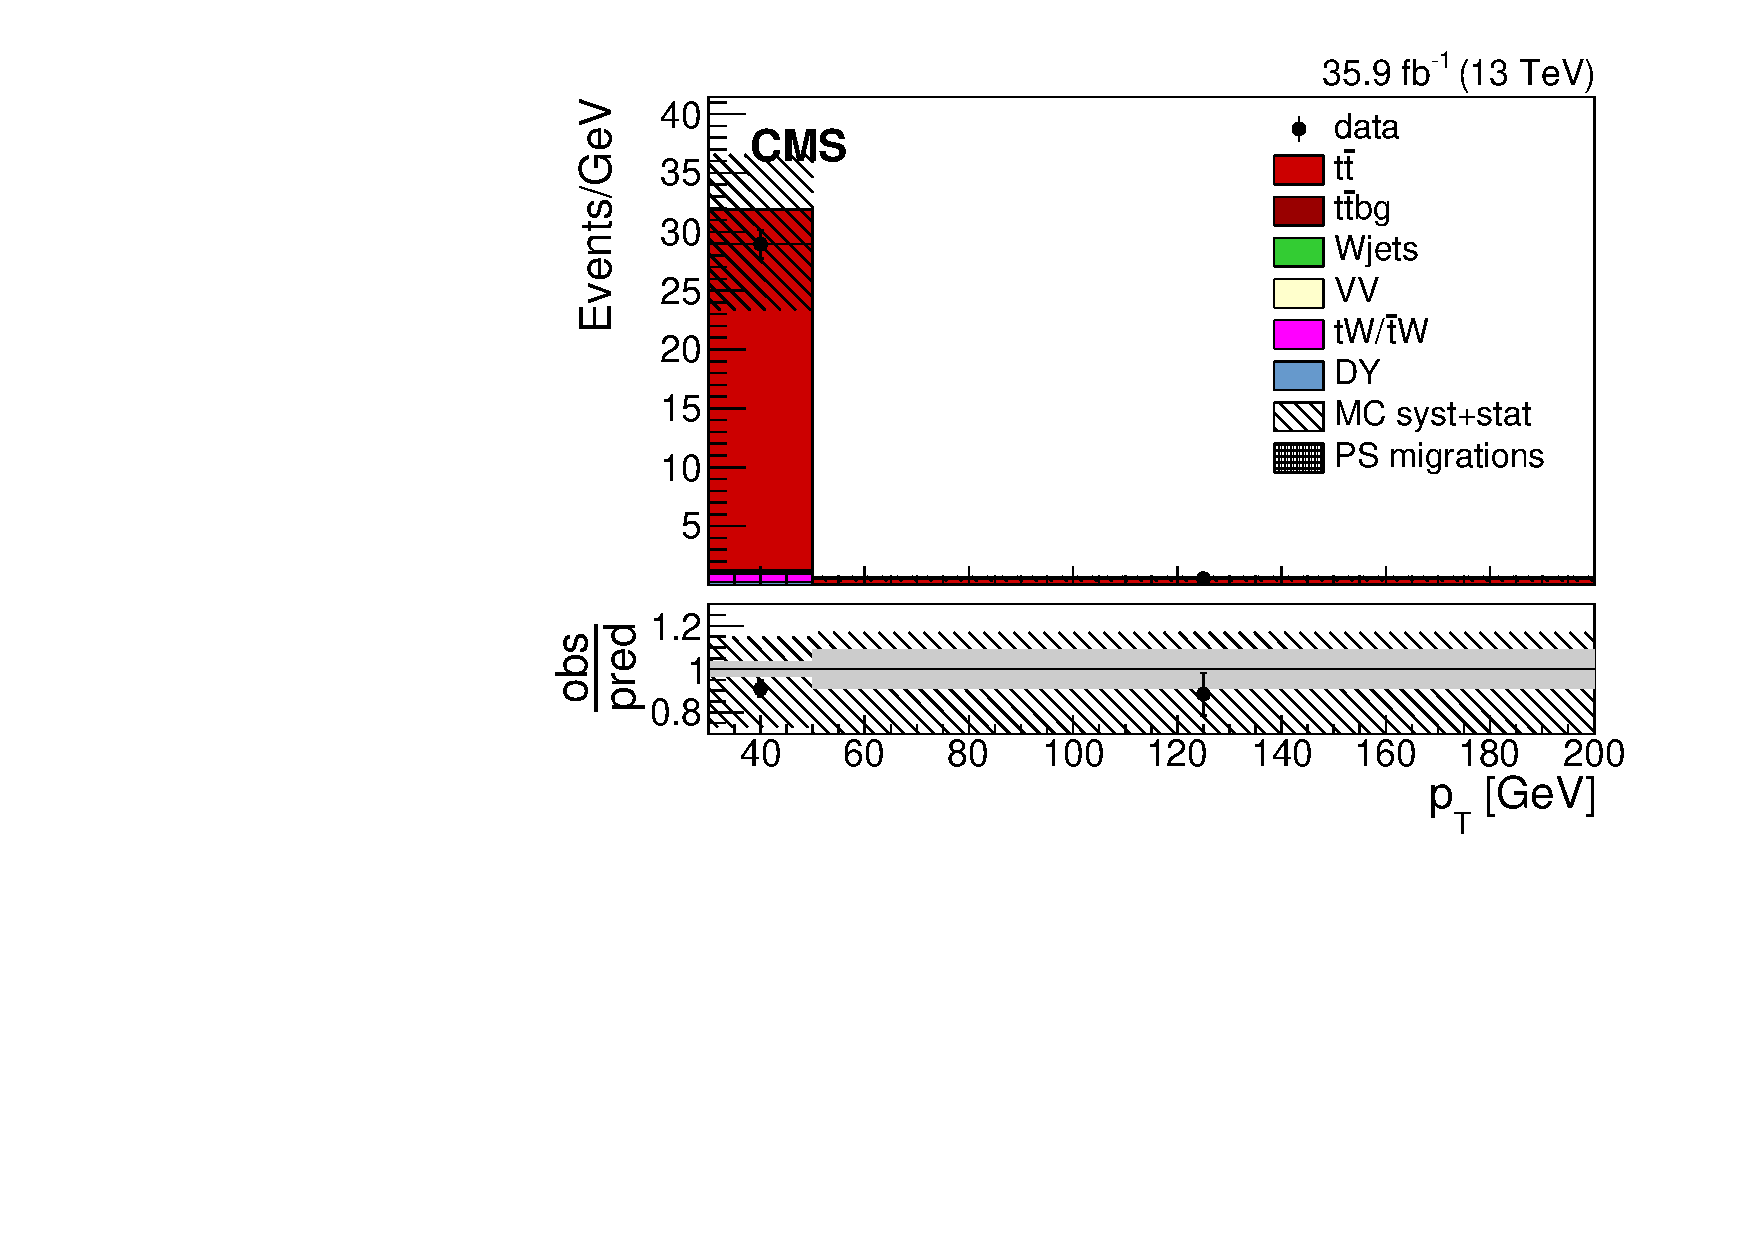
\includegraphics{CrossSection/Figures/ControlPlots/mumu_sysnom/third_jet_pt_2_3_b-jets_step_8.pdf}}  
\caption{Template distributions for events in the \mumu channel with one b-tagged jet (left column) or three b-tagged jets (right column). The distributions show the total event yield for zero (top) nd the trailing jet pt for one (second from top),
  two (second from bottom) or three or more (bottom) additional jets. 
  The hatched bands correspond to the total uncertainty on the predicted number of events. The ratios of the event yields in data and the sum of the
  predicted yields are shown at the bottom of each plot. Here, the solid
  gray band represents the contribution of the statistical uncertainty.  
       \label{fig:xsec_mumu_inputdistr}}
  \end{center}
\end{figure}

\begin{figure}[htbp!]
  \begin{center}
    \resizebox{0.4 \textwidth}{!}{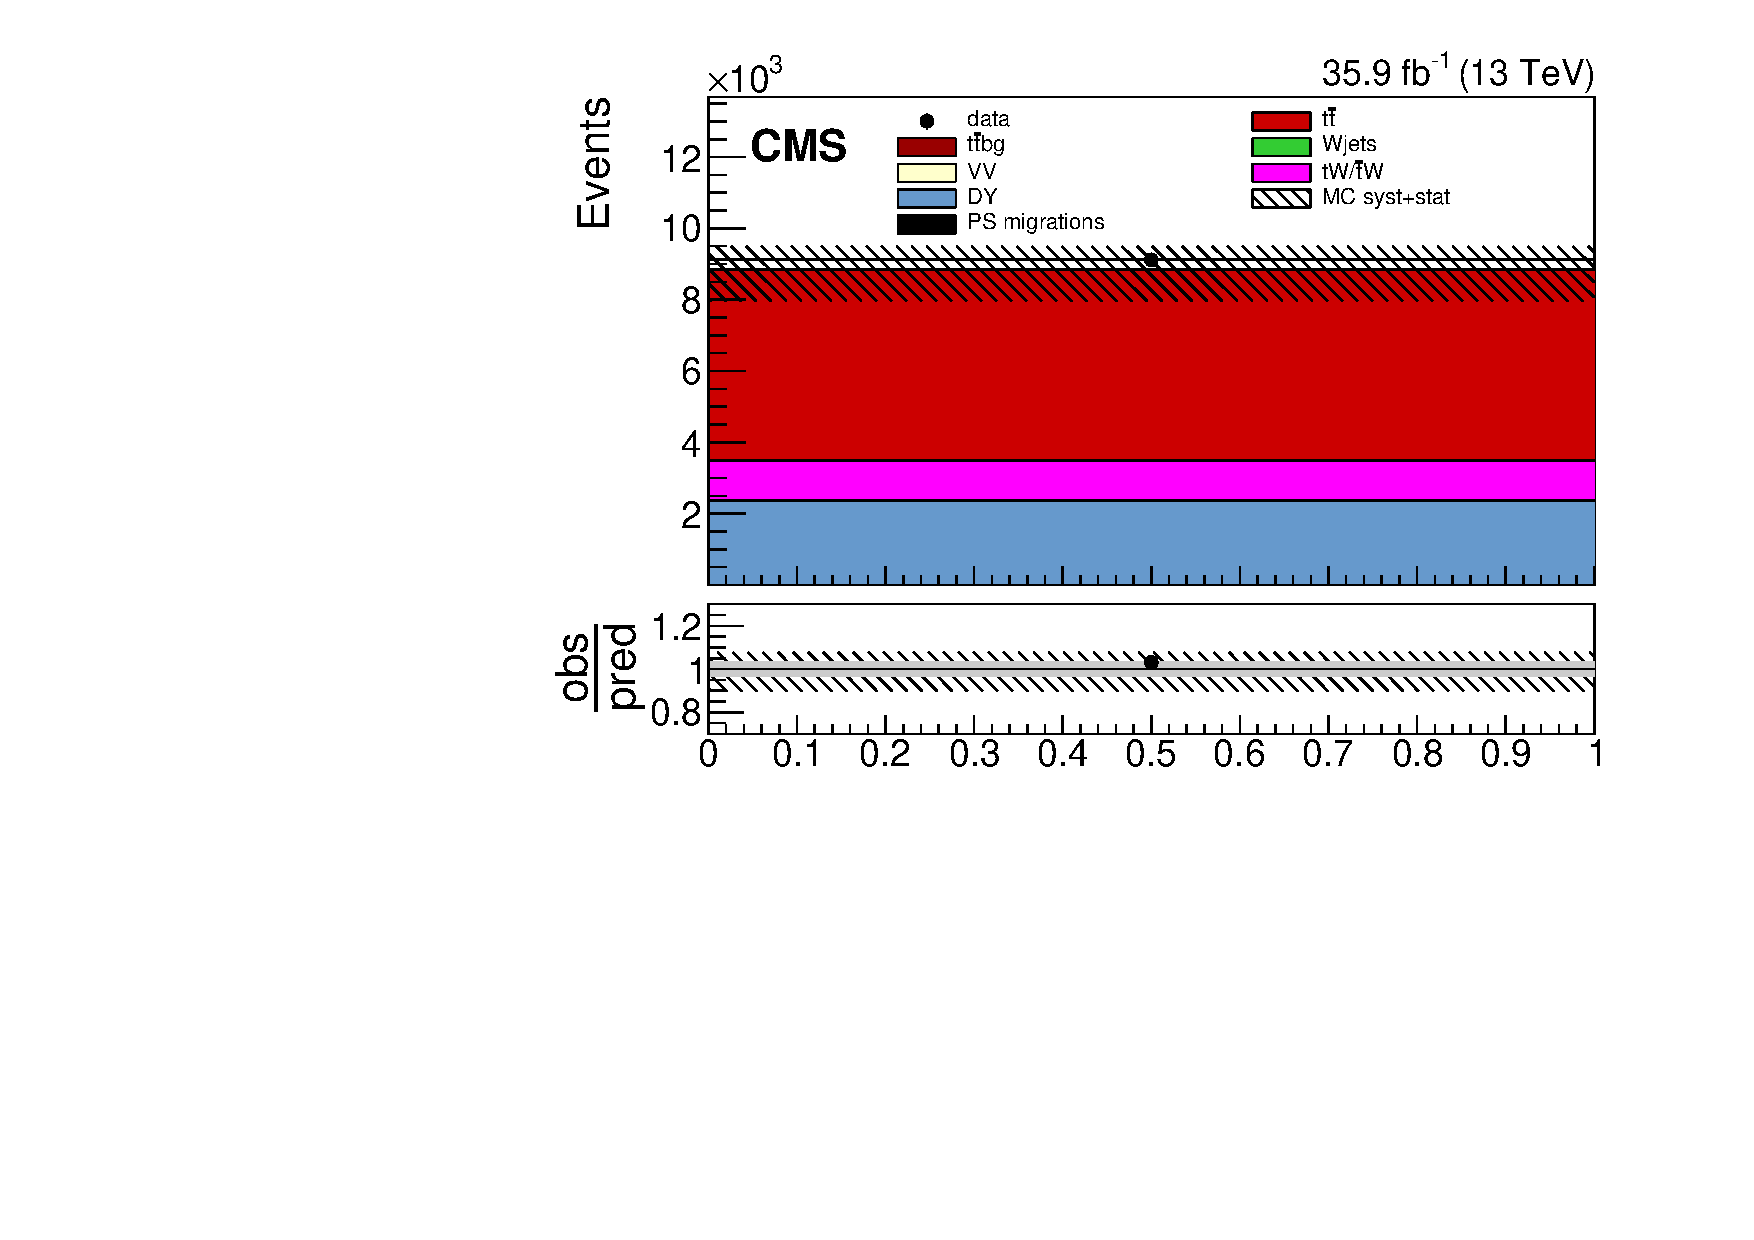
\includegraphics{CrossSection/Figures/ControlPlots/ee_sysnom/total_1_0_b-jets_step_8.pdf}}
    \resizebox{0.4 \textwidth}{!}{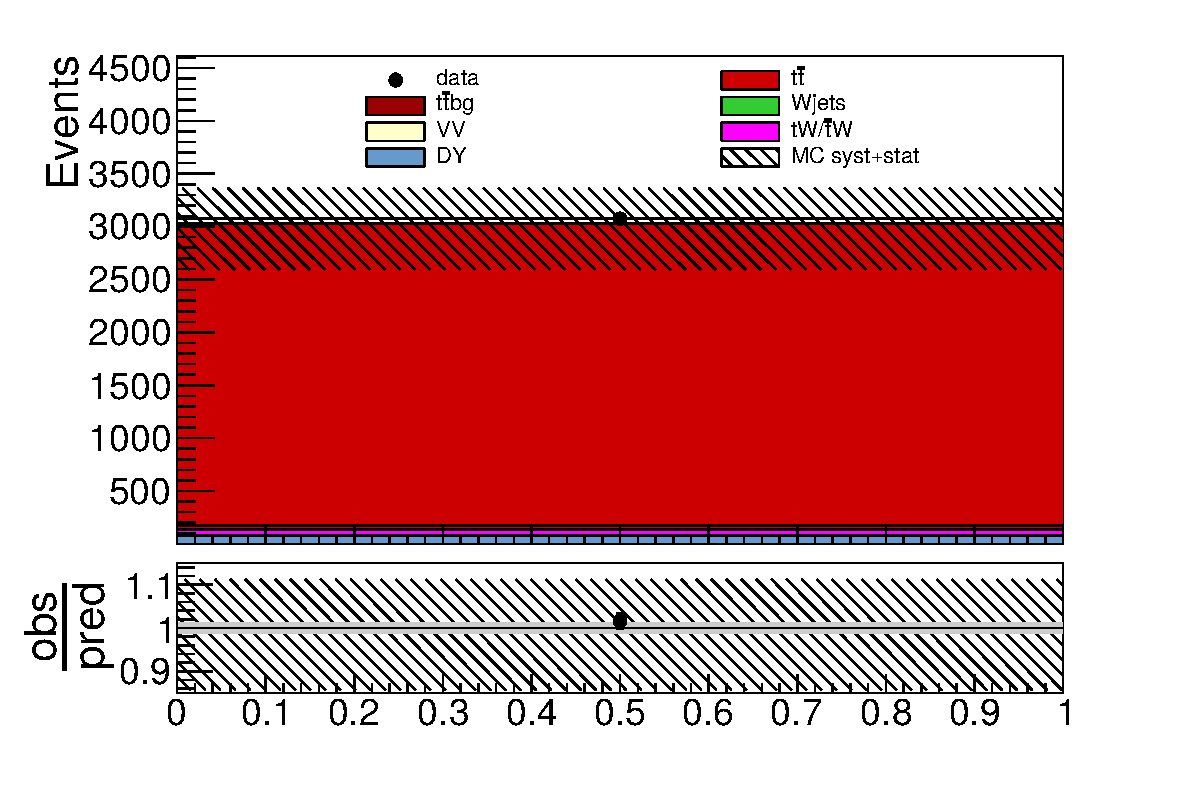
\includegraphics{CrossSection/Figures/ControlPlots/ee_sysnom/total_2_0_b-jets_step_8.pdf}}\\

    \resizebox{0.4 \textwidth}{!}{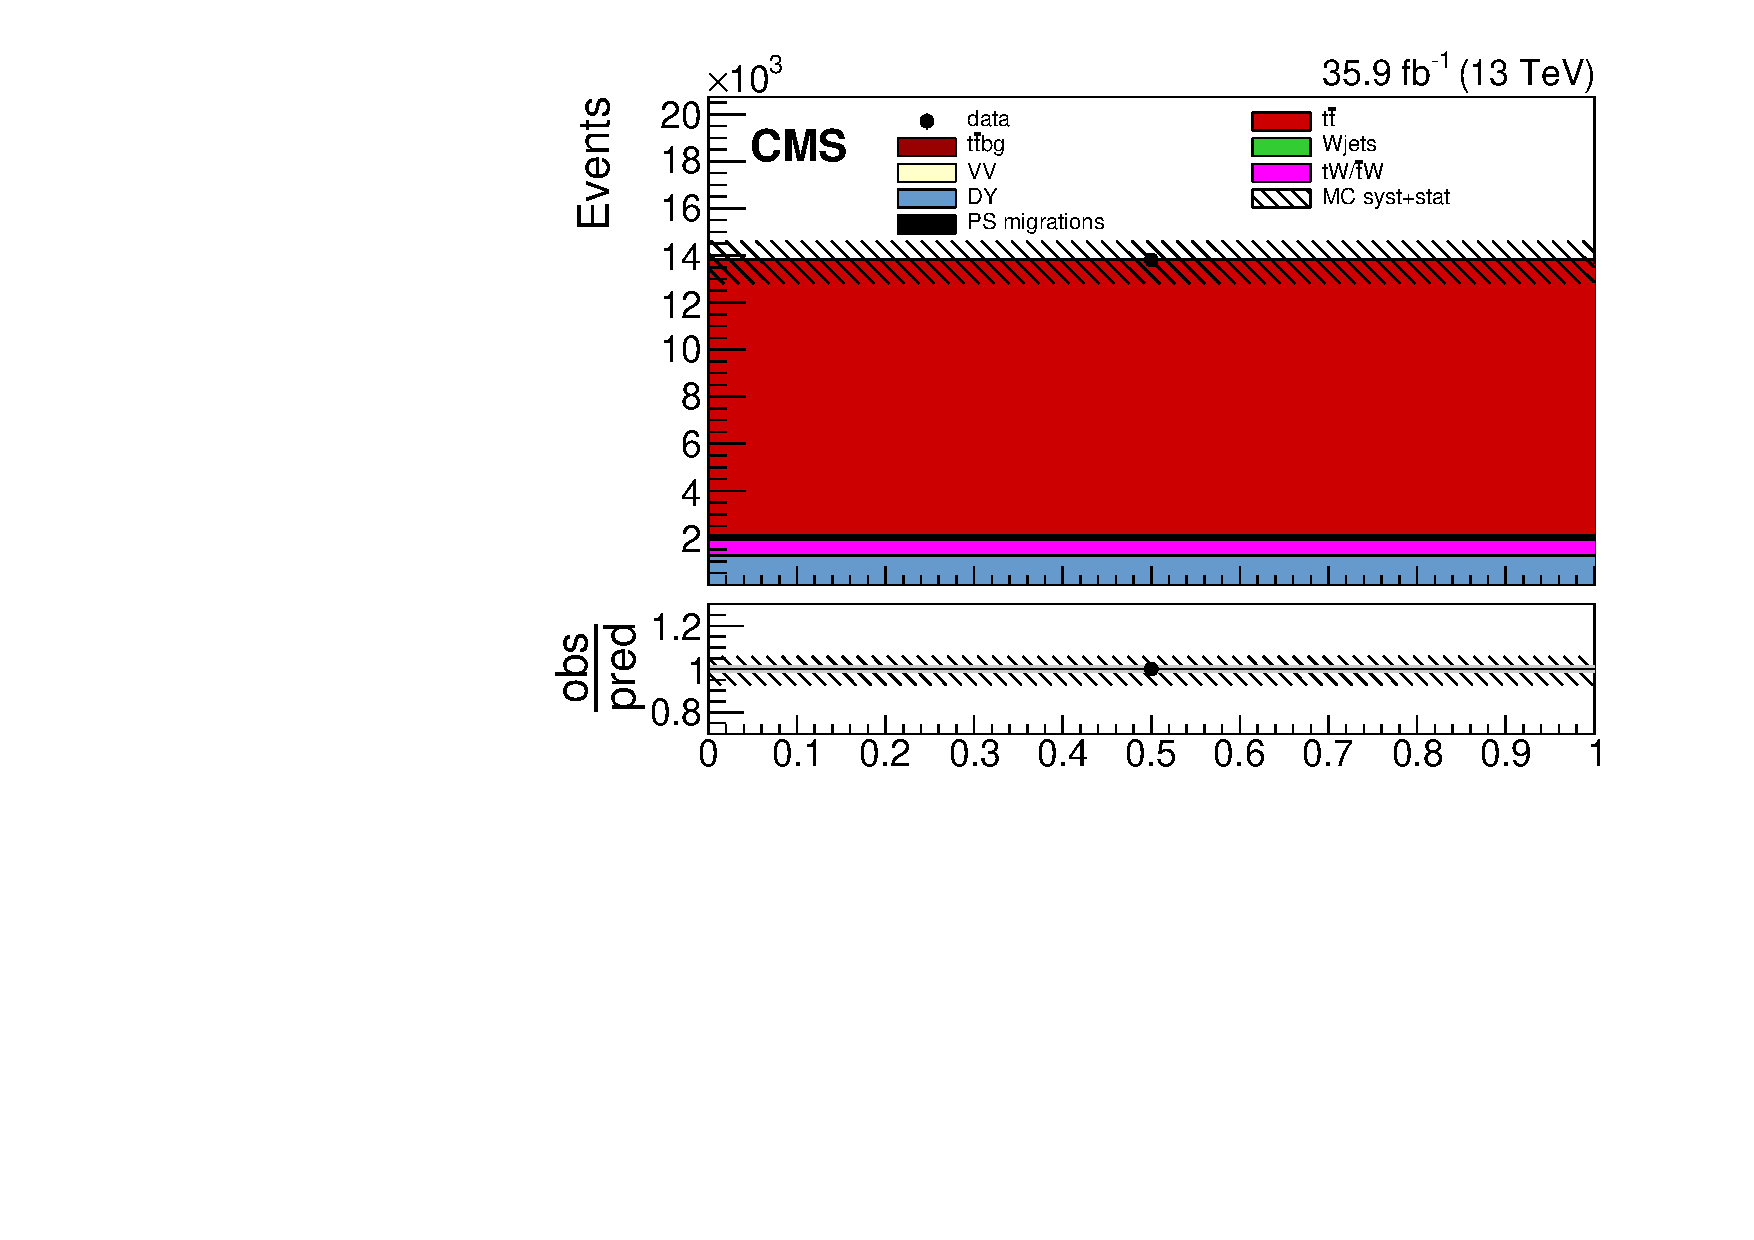
\includegraphics{CrossSection/Figures/ControlPlots/ee_sysnom/total_1_1_b-jets_step_8.pdf}}
    \resizebox{0.4 \textwidth}{!}{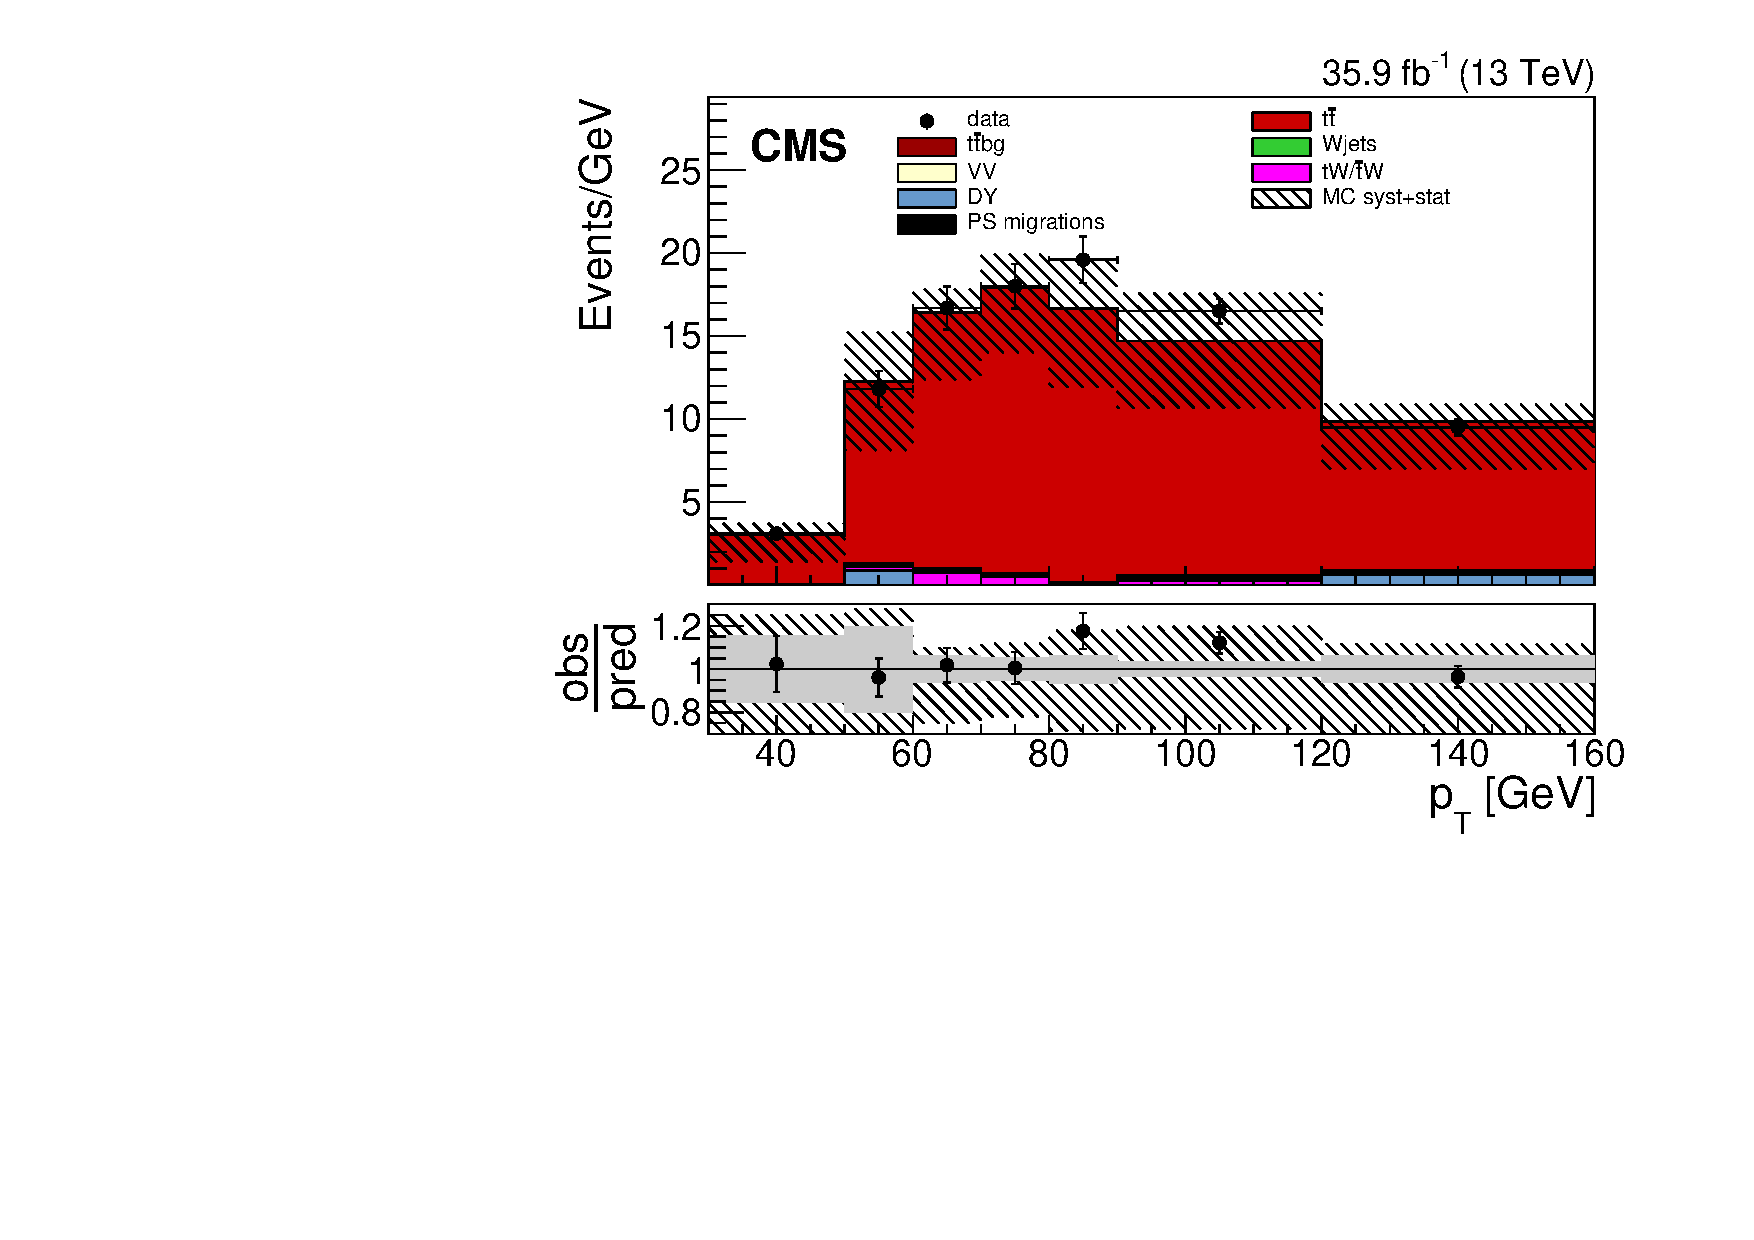
\includegraphics{CrossSection/Figures/ControlPlots/ee_sysnom/lead_jet_pt_2_1_b-jets_step_8.pdf}}\\
        
    \resizebox{0.4 \textwidth}{!}{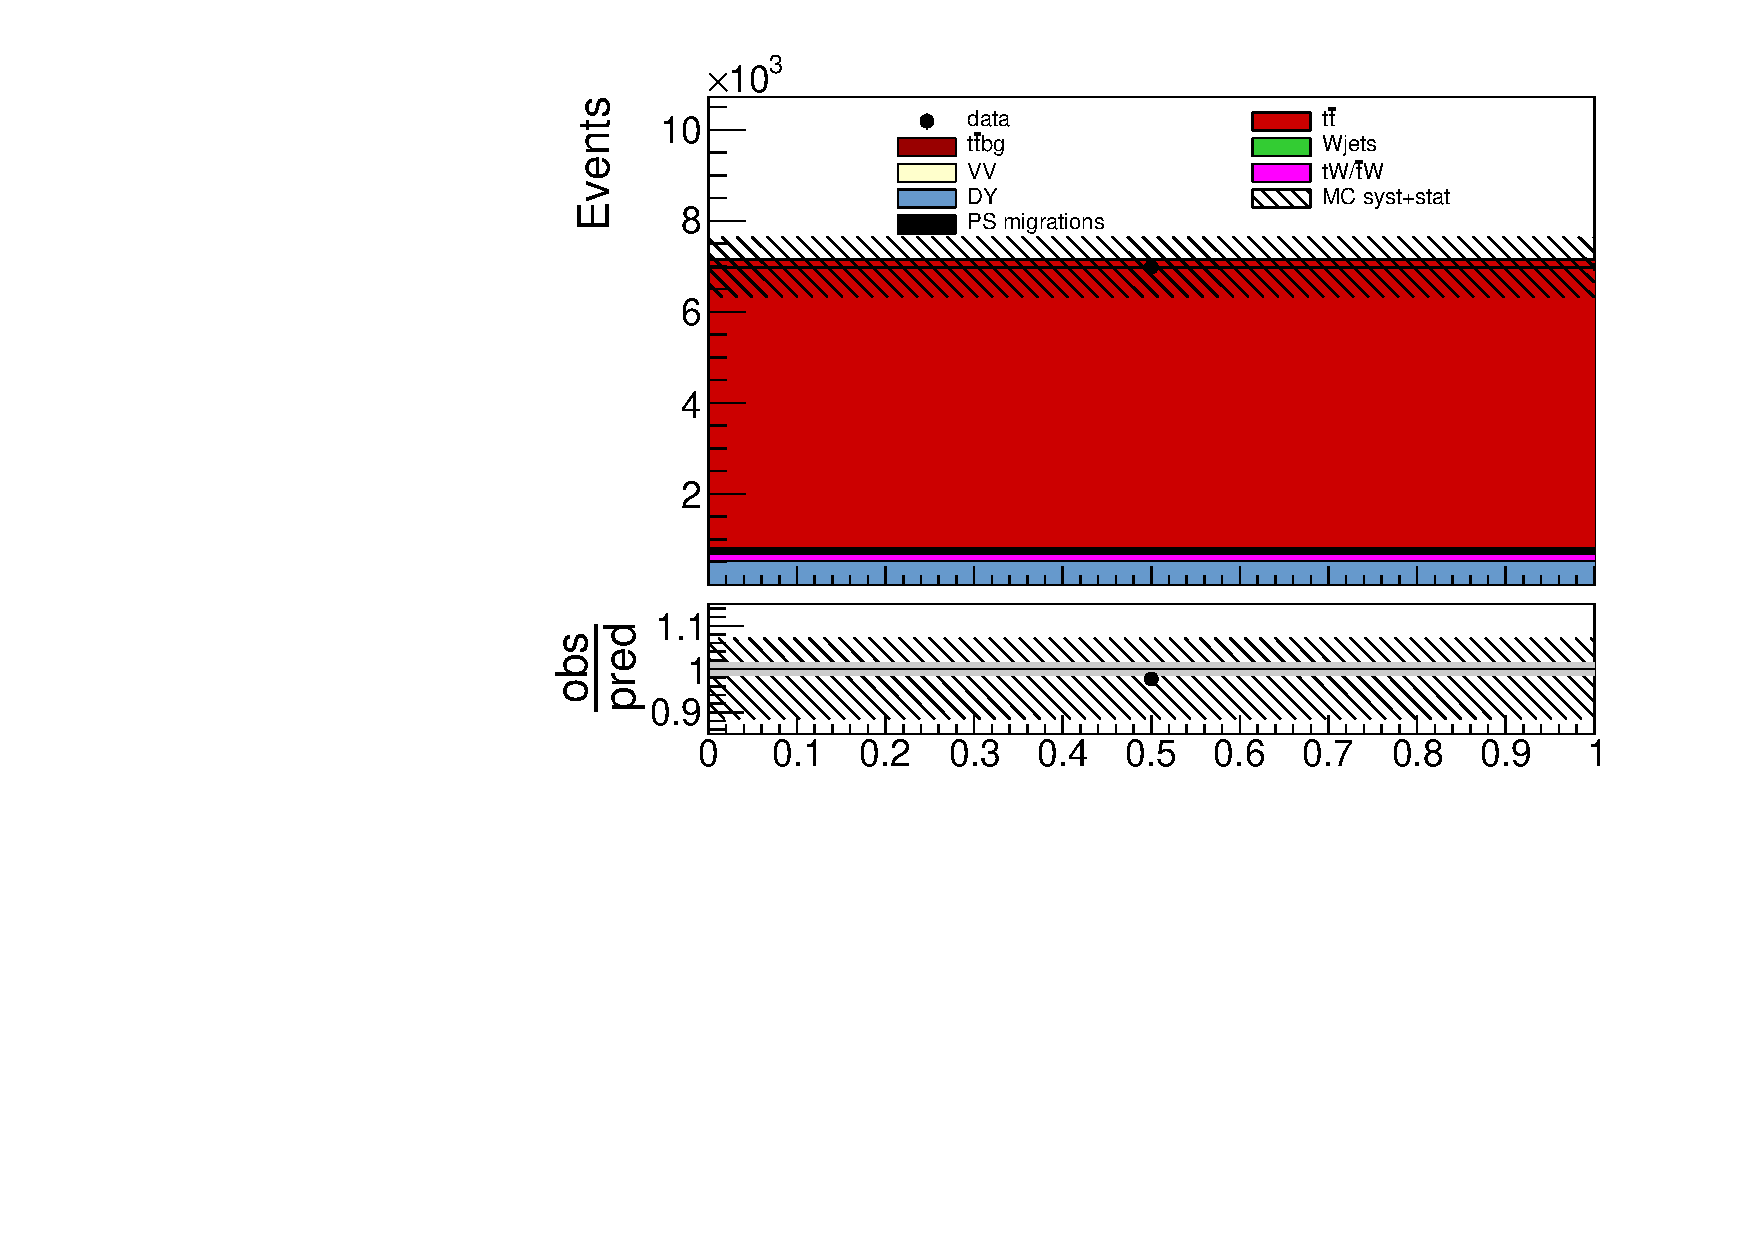
\includegraphics{CrossSection/Figures/ControlPlots/ee_sysnom/total_1_2_b-jets_step_8.pdf}}
    \resizebox{0.4 \textwidth}{!}{\includegraphics{CrossSection/Figures/ControlPlots/ee_sysnom/second_jet_pt_2_2_b-jets_step_8.pdf}}\\

    \resizebox{0.4 \textwidth}{!}{\includegraphics{CrossSection/Figures/ControlPlots/ee_sysnom/total_1_3_b-jets_step_8.pdf}}
    \resizebox{0.4 \textwidth}{!}{\includegraphics{CrossSection/Figures/ControlPlots/ee_sysnom/third_jet_pt_2_3_b-jets_step_8.pdf}} 
\caption{Template distributions for events in the \ee channel with one b-tagged jet (left column) or three b-tagged jets (right column). The distributions show the total event yield for zero (top) nd the trailing jet pt for one (second from top),
  two (second from bottom) or three or more (bottom) additional jets. 
  The hatched bands correspond to the total uncertainty on the predicted number of events. The ratios of the event yields in data and the sum of the
  predicted yields are shown at the bottom of each plot. Here, the solid
  gray band represents the contribution of the statistical uncertainty.  
       \label{fig:xsec_ee_inputdistr}}
  \end{center}
\end{figure}


    
\section{Definition of the $\chi^2$ Function}
\label{sec:xsec_stat}

A binned $\chi^2$ fit is used to extract the cross section and other free parameters.
The following expression is minimised:

\begin{eqnarray}
  \chi^2  &=& \sum_{i} \frac{(n_i-\mu_i)^2}{n_i + \delta_{\mu_i}^2} + \sum_{l} \pi(\omega_l) + \sum_{m} \pi(\lambda_m) \\
  \mu_i &=& s_i(\stt,\vec{\lambda}) + \sum_{l} b_{l,i}(\omega_l,\vec{\lambda})
\label{eq:xsec_chisqfunct}
\end{eqnarray}

Here the index $i$ represents a single bin, while $n_i$ is the number of measured events in data. The symbol $\mu_i$ represents the number
of expected events in simulation. The statistical uncertainty on the expected number of events is introduced in the term $\delta_{\mu_i}$ The terms $\omega_l$ denote the uncertainty on the normalisation of the background contribution and $\lambda_m$
denotes the penalty terms for nuisance parameters with Gaussian priors. For these nuisance parameters a unit normal distribution is chosen as penalty term. Nuisance parameters with a uniform prior do not contribute to the penalty terms.
The second equation breaks down the expected number of events $\mu_i$ per bin $i$ into the number of signal events $s_i$ depending on the \ttbar cross section $\stt$ and the nuisance parameters $\vec{\lambda}$ and the number of
background events  $b_{l,i}$ for each background process $l$ also depending on the nuisance parameters and the normalisation of the respective background process $\omega_l$.

In general nuisance parameters related to the detector affect both background and signal, while uncertainties affecting the theory predictions only affect the respective background or signal prediction (see Section \todo{Link to systematics chapter}).


The number of background events as used in Equation \ref{eq:xsec_expectev} can be decomposed as :

\begin{equation}
b_{l,i} = b_{l,i}^{MC} \cdot (1 + \omega_l),
\label{eq:nbli}
\end{equation}

Here $b_{l,i}^{MC}$ denotes the expected number of events from the simulation of the respective background process and $\omega_l$ denotes its normalization including the uncertainty.

Following the description in Section \ref{sec:xsec_templates}  the number of signal events is further devided according to the number of b-tagged jets.
The number of events in the categories for events with zero or more than two b-tagged jets $s_{0,b}$, for events with exactly one $s_{1,b}$ and for events with exactly two b-tagged jets $s_{2,b}$ are expressed as follows. Only events in the \emu channel contribute to category $s_{0,b}$.

\begin{eqnarray}
s_{0,b}  &=& \mathcal{L}_{\rm int}\stt \epsilon_{e\mu} \cdot (1-2\epsilon_b(1-C_b\epsilon_b)-C_b\epsilon_b^2) \\
s_{1,b}  &=& \mathcal{L}_{\rm int} \stt \epsilon_{ll} \cdot 2 \epsilon_b(1-C_b\epsilon_b) \\
s_{2,b}  &=& \mathcal{L}_{\rm int} \stt \epsilon_{ll} \cdot   \epsilon_b^2 C_b 
\label{eq:xsec_nb}.
\end{eqnarray}

Here $\mathcal{L}_{\rm int}$ is the integrated luminosity, $\stt$ is the visible \ttbar cross section and $\epsilon_{ll}$ is the efficiency of the dilepton selection.
The b-tag efficiency $\epsilon_b$ is the probability to reconstruct a b-tagged jet in a \ttbar event. It includes the efficiency of the b-tagging algorithm, the geometrical acceptance of the kinematic cuts on the b-jet ($\pt > 30\; \GeV, |\eta|<2.4$) and the probability of a light jet to be b-tagged (mis-tagging). In general the contribution of the geometrical acceptance and the mis-tag rate is comparatively low.
It is assumed that the two b-jets can be identified independently of each other. Remaining correlations are described by the parameter $C_b$ which is
$C_b=4s_{ll}s_{2,b}/(s_{1,b}+2s_{2,b})^2$ where $s_{ll}$ is the total number of selected events. 


Within the fit, the MC simulated quantities $\epsilon_{ll}$, $b_{l,i}$ and $s_{i}$ are taken from simulation and depend on the nuisance parameters $\vec{\lambda}$ in each bin.

The dependence of the template distributions on the nuisance parameters is modeled with a second order polynomial which is constructed using the nominal and the two systematically varied values of each nuisance parameters $\lambda_m=0,1,-1$.
The variation of the respective template distributions in each bin depends on the value of $\lambda$, with $\lambda = \pm 1$ corresponding to a $ \pm 1 \cdot \sigma$ variation. If multiple templates distributions are affected by one uncertainty or nuisance parameter all of them are varied coherently.
The template distributions are then added up to the expected number of events in each bin, as shhown in Equation \ref{eq:xsec_chisqfunct}. The expected number of events consequently mirrors the dependence of the template distributions on the nuisance parameters.
Some nuisance parameters are based on a one-sided variation so one systematically varied value exists. In these cases the dependence of the template distributions on the nuisance parameters is modeled by a linear function.

The MINUIT~\cite{James:1975dr} algorithm is used to minimize the  $\chi^2$ term (see \ref{eq:xsec_chisqfunct} ) as function of the free fit parameters $\stt$, $\vec{\omega}$
and $\vec{\lambda}$. 

\todo{Describe stat model when its final}


\section{Extrapolation from the visible to the Full Phase Space}
\label{sec:xsec_extraction}

The previous explanation only dealt with the visible cross section in the visible phase space. In order to extrapolate that result to the full phase space the acceptance
needs to be considered.

The acceptance can be introduced by replacing the efficiency of the dilepton selection as follows:

\begin{equation}
\epsilon_{ll} = A_{ll} \epsilon^{vis}_{ll}.
\label{eq:epsacc}
\end{equation}

Here $A_{ll}$ is the acceptance and $\epsilon^{vis}_{ll}$ is the efficiency in the visible phase space, with both depending on the nuisance parameters $\vec{\lambda}$.
The acceptance is defined by the kinematic selection requirements on the leptons as given in Section \ref{sec:xsec_sel} applied on the simulation. Specifically the cuts are applied after the parton shower and before the simulation of the detector \todo{Link to simulation description}. There the two leptons are required to be part of the $t \rightarrow W b$ decay. They are further required to be within $|\eta|< 2.4$ with the 
leading lepton having $\pt > 25 \; \GeV$ and the trailing lepton $\pt > 20 \; \GeV$. The invariant mass of the dilepton system is required to be $\mll > 20 \; \GeV$.
These cuts correspond to the selection in the \emu decay channel.

Since the acceptance should only be constrained within the visible phase space, it should be unconstrained for the extrapolation.
This applies to uncertainties on the theory prediction which affect the fraction of events in the visible phase space, especially the variation
of parameters in the matrix element generation and in the parton shower.

Overall the following uncertainties need to be extrapolated: \todo{List of uncerts, with names from syst chamber}

The extrapolation of the uncertainties takes the fitted value of each relevant nuisance parameter as central value. Then the change of acceptance for the explicit $\pm 1 \sigma$ variation is considered as the $\pm 1 \sigma$ variation on the acceptance. These additional uncertainties are then added to the result from the fit in the fiducial phase space for each relevant nuisance parameter. These additional uncertainties are treated as uncorrelated and each is added in quadrature to the result in the fiducial phase space. This procedure can lead to assymetrical variations, even for originally symmetrical nuisance parameter in case the fitted value of the nuisance parameter is not the original central value.




